% **************************************************************************************************************
% A Classic Thesis Style
% An Homage to The Elements of Typographic Style
%
% Copyright (C) 2017 André Miede and Ivo Pletikosić
%
% If you like the style then I would appreciate a postcard. My address
% can be found in the file ClassicThesis.pdf. A collection of the
% postcards I received so far is available online at
% http://postcards.miede.de
%
% License:
% This program is free software; you can redistribute it and/or modify
% it under the terms of the GNU General Public License as published by
% the Free Software Foundation; either version 2 of the License, or
% (at your option) any later version.
%
% This program is distributed in the hope that it will be useful,
% but WITHOUT ANY WARRANTY; without even the implied warranty of
% MERCHANTABILITY or FITNESS FOR A PARTICULAR PURPOSE.  See the
% GNU General Public License for more details.
%
% You should have received a copy of the GNU General Public License
% along with this program; see the file COPYING.  If not, write to
% the Free Software Foundation, Inc., 59 Temple Place - Suite 330,
% Boston, MA 02111-1307, USA.
%
% PLEASE SEE ALSO THE AUTHORS' NOTE REGARDING THIS LICENSE
% IN THE DOCUMENTATION (ClassicThesis.pdf --> Chapter 1 / Chapter01.tex)
% **************************************************************************************************************
\RequirePackage{silence} % :-\
    \WarningFilter{scrreprt}{Usage of package `titlesec'}
    %\WarningFilter{scrreprt}{Activating an ugly workaround}
    \WarningFilter{titlesec}{Non standard sectioning command detected}
\documentclass[ twoside,openright,titlepage,numbers=noenddot,headinclude,%1headlines,% letterpaper a4paper
                footinclude=true,cleardoublepage=empty,abstractoff, % <--- obsolete, remove (todo)
                BCOR=5mm,paper=a4,fontsize=11pt,%11pt,a4paper,%
                ngerman,american,%
                ]{scrreprt}
                
\usepackage[b5paper,layout=b5paper]{geometry}
%********************************************************************
% Note: Make all your adjustments in here
%*******************************************************
\usepackage{graphicx}
\usepackage{array}
\usepackage{multirow}
\usepackage[spanish, ruled, lined, onelanguage]{algorithm2e}
\usepackage[table]{xcolor}
\usepackage{anysize}
\usepackage{mathtools}
\usepackage{amsmath}
\usepackage{enumerate}
\usepackage{minted}
\usepackage{amssymb}
%Tablas
\usepackage{lscape}
\usepackage{geometry}
\usepackage{tablefootnote}

\usepackage{booktabs}
% ****************************************************************************************************
% classicthesis-config.tex
% formerly known as loadpackages.sty, classicthesis-ldpkg.sty, and classicthesis-preamble.sty
% Use it at the beginning of your ClassicThesis.tex, or as a LaTeX Preamble
% in your ClassicThesis.{tex,lyx} with % ****************************************************************************************************
% classicthesis-config.tex
% formerly known as loadpackages.sty, classicthesis-ldpkg.sty, and classicthesis-preamble.sty
% Use it at the beginning of your ClassicThesis.tex, or as a LaTeX Preamble
% in your ClassicThesis.{tex,lyx} with % ****************************************************************************************************
% classicthesis-config.tex
% formerly known as loadpackages.sty, classicthesis-ldpkg.sty, and classicthesis-preamble.sty
% Use it at the beginning of your ClassicThesis.tex, or as a LaTeX Preamble
% in your ClassicThesis.{tex,lyx} with \input{classicthesis-config}
% ****************************************************************************************************
% If you like the classicthesis, then I would appreciate a postcard.
% My address can be found in the file ClassicThesis.pdf. A collection
% of the postcards I received so far is available online at
% http://postcards.miede.de
% ****************************************************************************************************


% ****************************************************************************************************
% 0. Set the encoding of your files. UTF-8 is the only sensible encoding nowadays. If you can't read
% äöüßáéçèê∂åëæƒÏ€ then change the encoding setting in your editor, not the line below. If your editor
% does not support utf8 use another editor!
% ****************************************************************************************************
\PassOptionsToPackage{utf8}{inputenc}
  \usepackage{inputenc}

% ****************************************************************************************************
% 1. Configure classicthesis for your needs here, e.g., remove "drafting" below
% in order to deactivate the time-stamp on the pages
% (see ClassicThesis.pdf for more information):
% ****************************************************************************************************
\PassOptionsToPackage{
  drafting=false,    % print version information on the bottom of the pages
  tocaligned=false, % the left column of the toc will be aligned (no indentation)
  dottedtoc=false,  % page numbers in ToC flushed right
  parts=true,       % use part division
  eulerchapternumbers=true, % use AMS Euler for chapter font (otherwise Palatino)
  linedheaders=false,       % chaper headers will have line above and beneath
  floatperchapter=true,     % numbering per chapter for all floats (i.e., Figure 1.1)
  listings=true,    % load listings package and setup LoL
  subfig=true,      % setup for preloaded subfig package
  eulermath=false,  % use awesome Euler fonts for mathematical formulae (only with pdfLaTeX)
  beramono=true,    % toggle a nice monospaced font (w/ bold)
  minionpro=false   % setup for minion pro font; use minion pro small caps as well (only with pdfLaTeX)
}{classicthesis}


% ****************************************************************************************************
% 2. Personal data and user ad-hoc commands
% ****************************************************************************************************
\newcommand{\myTitle}{Análisis multimodal y multiobjetivo al problema del clustering con restricciones\xspace}
\newcommand{\mySubtitle}{An Homage to The Elements of Typographic Style\xspace}
\newcommand{\myDegree}{Graduado en Ingenieria\xspace}
\newcommand{\myName}{Alfonso García Martínez\xspace}
\newcommand{\myProf}{Put name here\xspace}
\newcommand{\myOtherProf}{Put name here\xspace}
\newcommand{\mySupervisor}{Put name here\xspace}
\newcommand{\myFaculty}{ETSIIT\xspace}
\newcommand{\myDepartment}{Decsai\xspace}
\newcommand{\myUni}{Universidad de Granada\xspace}
\newcommand{\myLocation}{Granada\xspace}
\newcommand{\myTime}{Septiembre 2021\xspace}
\newcommand{\myVersion}{version 4.4}

% ********************************************************************
% Setup, finetuning, and useful commands
% ********************************************************************
\newcounter{dummy} % necessary for correct hyperlinks (to index, bib, etc.)
\newlength{\abcd} % for ab..z string length calculation
\providecommand{\mLyX}{L\kern-.1667em\lower.25em\hbox{Y}\kern-.125emX\@}
\newcommand{\ie}{i.\,e.}
\newcommand{\Ie}{I.\,e.}
\newcommand{\eg}{e.\,g.}
\newcommand{\Eg}{E.\,g.}
% ****************************************************************************************************


% ****************************************************************************************************
% 3. Loading some handy packages
% ****************************************************************************************************
% ********************************************************************
% Packages with options that might require adjustments
% ********************************************************************
%\PassOptionsToPackage{ngerman,american}{babel}   % change this to your language(s), main language last
% Spanish languages need extra options in order to work with this template
\PassOptionsToPackage{spanish,es-lcroman, es-tabla}{babel}
    \usepackage{babel}

\usepackage{csquotes}
\PassOptionsToPackage{%
  %backend=biber,bibencoding=utf8, %instead of bibtex
  backend=bibtex8,bibencoding=ascii,%
  language=auto,%
  style=numeric-comp,%
  %style=authoryear-comp, % Author 1999, 2010
  %bibstyle=authoryear,dashed=false, % dashed: substitute rep. author with ---
  sorting=none, % name, year, title
  maxbibnames=10, % default: 3, et al.
  %backref=true,%
  natbib=true % natbib compatibility mode (\citep and \citet still work)
}{biblatex}
    \usepackage{biblatex}
    
\PassOptionsToPackage{fleqn}{amsmath}       % math environments and more by the AMS
  \usepackage{amsmath}

% ********************************************************************
% General useful packages
% ********************************************************************
\PassOptionsToPackage{T1}{fontenc} % T2A for cyrillics
  \usepackage{fontenc}
\usepackage{textcomp} % fix warning with missing font shapes
\usepackage{scrhack} % fix warnings when using KOMA with listings package
\usepackage{xspace} % to get the spacing after macros right
\usepackage{mparhack} % get marginpar right
%\usepackage{fixltx2e} % fixes some LaTeX stuff --> since 2015 in the LaTeX kernel (see below)
% \usepackage[latest]{latexrelease} % emulate newer kernel version if older is detected
\PassOptionsToPackage{printonlyused,smaller}{acronym}
  \usepackage{acronym} % nice macros for handling all acronyms in the thesis
  %\renewcommand{\bflabel}[1]{{#1}\hfill} % fix the list of acronyms --> no longer working
  %\renewcommand*{\acsfont}[1]{\textsc{#1}}
  %\renewcommand*{\aclabelfont}[1]{\acsfont{#1}}
  %\def\bflabel#1{{#1\hfill}}
  \def\bflabel#1{{\acsfont{#1}\hfill}}
  \def\aclabelfont#1{\acsfont{#1}}
% ****************************************************************************************************
%\usepackage{pgfplots} % External TikZ/PGF support (thanks to Andreas Nautsch)
%\usetikzlibrary{external}
%\tikzexternalize[mode=list and make, prefix=ext-tikz/]
% ****************************************************************************************************


% ****************************************************************************************************
% 4. Setup floats: tables, (sub)figures, and captions
% ****************************************************************************************************
\usepackage{tabularx} % better tables
  \setlength{\extrarowheight}{3pt} % increase table row height
\newcommand{\tableheadline}[1]{\multicolumn{1}{c}{\spacedlowsmallcaps{#1}}}
\newcommand{\myfloatalign}{\centering} % to be used with each float for alignment
\usepackage{caption}
% Thanks to cgnieder and Claus Lahiri
% http://tex.stackexchange.com/questions/69349/spacedlowsmallcaps-in-caption-label
% [REMOVED DUE TO OTHER PROBLEMS, SEE ISSUE #82]
%\DeclareCaptionLabelFormat{smallcaps}{\bothIfFirst{#1}{~}\MakeTextLowercase{\textsc{#2}}}
%\captionsetup{font=small,labelformat=smallcaps} % format=hang,
\captionsetup{font=small} % format=hang,
\usepackage{subfig}
% ****************************************************************************************************


% ****************************************************************************************************
% 5. Setup code listings
% ****************************************************************************************************
\usepackage{listings}
%\lstset{emph={trueIndex,root},emphstyle=\color{BlueViolet}}%\underbar} % for special keywords
\lstset{language=[LaTeX]Tex,%C++,
  morekeywords={PassOptionsToPackage,selectlanguage},
  keywordstyle=\color{RoyalBlue},%\bfseries,
  basicstyle=\small\ttfamily,
  %identifierstyle=\color{NavyBlue},
  commentstyle=\color{Green}\ttfamily,
  stringstyle=\rmfamily,
  numbers=none,%left,%
  numberstyle=\scriptsize,%\tiny
  stepnumber=5,
  numbersep=8pt,
  showstringspaces=false,
  breaklines=true,
  %frameround=ftff,
  %frame=single,
  belowcaptionskip=.75\baselineskip
  %frame=L
}
% ****************************************************************************************************


% ****************************************************************************************************
% 6. PDFLaTeX, hyperreferences, and citation backreferences
% ****************************************************************************************************
% ********************************************************************
% Using PDFLaTeX
% ********************************************************************
\PassOptionsToPackage{hyperfootnotes=false,pdfpagelabels}{hyperref}
  \usepackage{hyperref}  % backref linktocpage pagebackref
%\ifpdf
%\pdfcompresslevel=9
%\pdfadjustspacing=1
%\fi
%\PassOptionsToPackage{pdftex}{graphicx} %%%IVO: driver will be chosen automatically
  \usepackage{graphicx}


% ********************************************************************
% Hyperreferences
% ********************************************************************
\hypersetup{%
  %draft, % hyperref's draft mode, for printing see below
  colorlinks=true, linktocpage=true, pdfstartpage=3, pdfstartview=FitV,%
  % uncomment the following line if you want to have black links (e.g., for printing)
  %colorlinks=false, linktocpage=false, pdfstartpage=3, pdfstartview=FitV, pdfborder={0 0 0},%
  breaklinks=true, pdfpagemode=UseNone, pageanchor=true, pdfpagemode=UseOutlines,%
  plainpages=false, bookmarksnumbered, bookmarksopen=true, bookmarksopenlevel=1,%
  hypertexnames=true, pdfhighlight=/O,%nesting=true,%frenchlinks,%
  urlcolor=webbrown, linkcolor=black, citecolor=black, %pagecolor=RoyalBlue,%
  %urlcolor=Black, linkcolor=Black, citecolor=Black, %pagecolor=Black,%
  pdftitle={\myTitle},%
  pdfauthor={\textcopyright\ \myName, \myUni, \myFaculty},%
  pdfsubject={},%
  pdfkeywords={},%
  pdfcreator={pdfLaTeX},%
  pdfproducer={LaTeX with hyperref and classicthesis}%
}

% ********************************************************************
% Setup autoreferences
% ********************************************************************
% There are some issues regarding autorefnames
% http://www.ureader.de/msg/136221647.aspx
% http://www.tex.ac.uk/cgi-bin/texfaq2html?label=latexwords
% you have to redefine the makros for the
% language you use, e.g., american, ngerman
% (as chosen when loading babel/AtBeginDocument)
% ********************************************************************
\makeatletter
\@ifpackageloaded{babel}%
  {%
    \addto\extrasamerican{%
      \renewcommand*{\figureautorefname}{Figure}%
      \renewcommand*{\tableautorefname}{Table}%
      \renewcommand*{\partautorefname}{Part}%
      \renewcommand*{\chapterautorefname}{Chapter}%
      \renewcommand*{\sectionautorefname}{Section}%
      \renewcommand*{\subsectionautorefname}{Section}%
      \renewcommand*{\subsubsectionautorefname}{Section}%
    }%
    \addto\extrasngerman{%
      \renewcommand*{\paragraphautorefname}{Absatz}%
      \renewcommand*{\subparagraphautorefname}{Unterabsatz}%
      \renewcommand*{\footnoteautorefname}{Fu\"snote}%
      \renewcommand*{\FancyVerbLineautorefname}{Zeile}%
      \renewcommand*{\theoremautorefname}{Theorem}%
      \renewcommand*{\appendixautorefname}{Anhang}%
      \renewcommand*{\equationautorefname}{Gleichung}%
      \renewcommand*{\itemautorefname}{Punkt}%
    }%
      % Fix to getting autorefs for subfigures right (thanks to Belinda Vogt for changing the definition)
      \providecommand{\subfigureautorefname}{\figureautorefname}%
    }{\relax}
\makeatother


% ****************************************************************************************************
% 7. Last calls before the bar closes
% ****************************************************************************************************
% ********************************************************************
% Development Stuff
% ********************************************************************
\listfiles
%\PassOptionsToPackage{l2tabu,orthodox,abort}{nag}
%  \usepackage{nag}
%\PassOptionsToPackage{warning, all}{onlyamsmath}
%  \usepackage{onlyamsmath}

% ********************************************************************
% Last, but not least...
% ********************************************************************
\usepackage[dottedtoc]{classicthesis}
% ****************************************************************************************************


% ****************************************************************************************************
% 8. Further adjustments (experimental)
% ****************************************************************************************************
% ********************************************************************
% Changing the text area
% ********************************************************************
%\areaset[current]{312pt}{761pt} % 686 (factor 2.2) + 33 head + 42 head \the\footskip
%\setlength{\marginparwidth}{7em}%
%\setlength{\marginparsep}{2em}%

% ********************************************************************
% Using different fonts
% ********************************************************************
%\usepackage[oldstylenums]{kpfonts} % oldstyle notextcomp
%\usepackage[osf]{libertine}
%\usepackage[light,condensed,math]{iwona}
%\renewcommand{\sfdefault}{iwona}
%\usepackage{lmodern} % <-- no osf support :-(
%\usepackage{cfr-lm} %
%\usepackage[urw-garamond]{mathdesign} <-- no osf support :-(
%\usepackage[default,osfigures]{opensans} % scale=0.95
%\usepackage[sfdefault]{FiraSans}
% ********************************************************************
% \usepackage[largesc,osf]{newpxtext}
% Used to fix these:
% https://bitbucket.org/amiede/classicthesis/issues/139/italics-in-pallatino-capitals-chapter
% https://bitbucket.org/amiede/classicthesis/issues/45/problema-testatine-su-classicthesis-style
% ********************************************************************
%\linespread{1.05} % a bit more for Palatino
% ****************************************************************************************************

% ****************************************************************************************************
% If you like the classicthesis, then I would appreciate a postcard.
% My address can be found in the file ClassicThesis.pdf. A collection
% of the postcards I received so far is available online at
% http://postcards.miede.de
% ****************************************************************************************************


% ****************************************************************************************************
% 0. Set the encoding of your files. UTF-8 is the only sensible encoding nowadays. If you can't read
% äöüßáéçèê∂åëæƒÏ€ then change the encoding setting in your editor, not the line below. If your editor
% does not support utf8 use another editor!
% ****************************************************************************************************
\PassOptionsToPackage{utf8}{inputenc}
  \usepackage{inputenc}

% ****************************************************************************************************
% 1. Configure classicthesis for your needs here, e.g., remove "drafting" below
% in order to deactivate the time-stamp on the pages
% (see ClassicThesis.pdf for more information):
% ****************************************************************************************************
\PassOptionsToPackage{
  drafting=false,    % print version information on the bottom of the pages
  tocaligned=false, % the left column of the toc will be aligned (no indentation)
  dottedtoc=false,  % page numbers in ToC flushed right
  parts=true,       % use part division
  eulerchapternumbers=true, % use AMS Euler for chapter font (otherwise Palatino)
  linedheaders=false,       % chaper headers will have line above and beneath
  floatperchapter=true,     % numbering per chapter for all floats (i.e., Figure 1.1)
  listings=true,    % load listings package and setup LoL
  subfig=true,      % setup for preloaded subfig package
  eulermath=false,  % use awesome Euler fonts for mathematical formulae (only with pdfLaTeX)
  beramono=true,    % toggle a nice monospaced font (w/ bold)
  minionpro=false   % setup for minion pro font; use minion pro small caps as well (only with pdfLaTeX)
}{classicthesis}


% ****************************************************************************************************
% 2. Personal data and user ad-hoc commands
% ****************************************************************************************************
\newcommand{\myTitle}{Análisis multimodal y multiobjetivo al problema del clustering con restricciones\xspace}
\newcommand{\mySubtitle}{An Homage to The Elements of Typographic Style\xspace}
\newcommand{\myDegree}{Graduado en Ingenieria\xspace}
\newcommand{\myName}{Alfonso García Martínez\xspace}
\newcommand{\myProf}{Put name here\xspace}
\newcommand{\myOtherProf}{Put name here\xspace}
\newcommand{\mySupervisor}{Put name here\xspace}
\newcommand{\myFaculty}{ETSIIT\xspace}
\newcommand{\myDepartment}{Decsai\xspace}
\newcommand{\myUni}{Universidad de Granada\xspace}
\newcommand{\myLocation}{Granada\xspace}
\newcommand{\myTime}{Septiembre 2021\xspace}
\newcommand{\myVersion}{version 4.4}

% ********************************************************************
% Setup, finetuning, and useful commands
% ********************************************************************
\newcounter{dummy} % necessary for correct hyperlinks (to index, bib, etc.)
\newlength{\abcd} % for ab..z string length calculation
\providecommand{\mLyX}{L\kern-.1667em\lower.25em\hbox{Y}\kern-.125emX\@}
\newcommand{\ie}{i.\,e.}
\newcommand{\Ie}{I.\,e.}
\newcommand{\eg}{e.\,g.}
\newcommand{\Eg}{E.\,g.}
% ****************************************************************************************************


% ****************************************************************************************************
% 3. Loading some handy packages
% ****************************************************************************************************
% ********************************************************************
% Packages with options that might require adjustments
% ********************************************************************
%\PassOptionsToPackage{ngerman,american}{babel}   % change this to your language(s), main language last
% Spanish languages need extra options in order to work with this template
\PassOptionsToPackage{spanish,es-lcroman, es-tabla}{babel}
    \usepackage{babel}

\usepackage{csquotes}
\PassOptionsToPackage{%
  %backend=biber,bibencoding=utf8, %instead of bibtex
  backend=bibtex8,bibencoding=ascii,%
  language=auto,%
  style=numeric-comp,%
  %style=authoryear-comp, % Author 1999, 2010
  %bibstyle=authoryear,dashed=false, % dashed: substitute rep. author with ---
  sorting=none, % name, year, title
  maxbibnames=10, % default: 3, et al.
  %backref=true,%
  natbib=true % natbib compatibility mode (\citep and \citet still work)
}{biblatex}
    \usepackage{biblatex}
    
\PassOptionsToPackage{fleqn}{amsmath}       % math environments and more by the AMS
  \usepackage{amsmath}

% ********************************************************************
% General useful packages
% ********************************************************************
\PassOptionsToPackage{T1}{fontenc} % T2A for cyrillics
  \usepackage{fontenc}
\usepackage{textcomp} % fix warning with missing font shapes
\usepackage{scrhack} % fix warnings when using KOMA with listings package
\usepackage{xspace} % to get the spacing after macros right
\usepackage{mparhack} % get marginpar right
%\usepackage{fixltx2e} % fixes some LaTeX stuff --> since 2015 in the LaTeX kernel (see below)
% \usepackage[latest]{latexrelease} % emulate newer kernel version if older is detected
\PassOptionsToPackage{printonlyused,smaller}{acronym}
  \usepackage{acronym} % nice macros for handling all acronyms in the thesis
  %\renewcommand{\bflabel}[1]{{#1}\hfill} % fix the list of acronyms --> no longer working
  %\renewcommand*{\acsfont}[1]{\textsc{#1}}
  %\renewcommand*{\aclabelfont}[1]{\acsfont{#1}}
  %\def\bflabel#1{{#1\hfill}}
  \def\bflabel#1{{\acsfont{#1}\hfill}}
  \def\aclabelfont#1{\acsfont{#1}}
% ****************************************************************************************************
%\usepackage{pgfplots} % External TikZ/PGF support (thanks to Andreas Nautsch)
%\usetikzlibrary{external}
%\tikzexternalize[mode=list and make, prefix=ext-tikz/]
% ****************************************************************************************************


% ****************************************************************************************************
% 4. Setup floats: tables, (sub)figures, and captions
% ****************************************************************************************************
\usepackage{tabularx} % better tables
  \setlength{\extrarowheight}{3pt} % increase table row height
\newcommand{\tableheadline}[1]{\multicolumn{1}{c}{\spacedlowsmallcaps{#1}}}
\newcommand{\myfloatalign}{\centering} % to be used with each float for alignment
\usepackage{caption}
% Thanks to cgnieder and Claus Lahiri
% http://tex.stackexchange.com/questions/69349/spacedlowsmallcaps-in-caption-label
% [REMOVED DUE TO OTHER PROBLEMS, SEE ISSUE #82]
%\DeclareCaptionLabelFormat{smallcaps}{\bothIfFirst{#1}{~}\MakeTextLowercase{\textsc{#2}}}
%\captionsetup{font=small,labelformat=smallcaps} % format=hang,
\captionsetup{font=small} % format=hang,
\usepackage{subfig}
% ****************************************************************************************************


% ****************************************************************************************************
% 5. Setup code listings
% ****************************************************************************************************
\usepackage{listings}
%\lstset{emph={trueIndex,root},emphstyle=\color{BlueViolet}}%\underbar} % for special keywords
\lstset{language=[LaTeX]Tex,%C++,
  morekeywords={PassOptionsToPackage,selectlanguage},
  keywordstyle=\color{RoyalBlue},%\bfseries,
  basicstyle=\small\ttfamily,
  %identifierstyle=\color{NavyBlue},
  commentstyle=\color{Green}\ttfamily,
  stringstyle=\rmfamily,
  numbers=none,%left,%
  numberstyle=\scriptsize,%\tiny
  stepnumber=5,
  numbersep=8pt,
  showstringspaces=false,
  breaklines=true,
  %frameround=ftff,
  %frame=single,
  belowcaptionskip=.75\baselineskip
  %frame=L
}
% ****************************************************************************************************


% ****************************************************************************************************
% 6. PDFLaTeX, hyperreferences, and citation backreferences
% ****************************************************************************************************
% ********************************************************************
% Using PDFLaTeX
% ********************************************************************
\PassOptionsToPackage{hyperfootnotes=false,pdfpagelabels}{hyperref}
  \usepackage{hyperref}  % backref linktocpage pagebackref
%\ifpdf
%\pdfcompresslevel=9
%\pdfadjustspacing=1
%\fi
%\PassOptionsToPackage{pdftex}{graphicx} %%%IVO: driver will be chosen automatically
  \usepackage{graphicx}


% ********************************************************************
% Hyperreferences
% ********************************************************************
\hypersetup{%
  %draft, % hyperref's draft mode, for printing see below
  colorlinks=true, linktocpage=true, pdfstartpage=3, pdfstartview=FitV,%
  % uncomment the following line if you want to have black links (e.g., for printing)
  %colorlinks=false, linktocpage=false, pdfstartpage=3, pdfstartview=FitV, pdfborder={0 0 0},%
  breaklinks=true, pdfpagemode=UseNone, pageanchor=true, pdfpagemode=UseOutlines,%
  plainpages=false, bookmarksnumbered, bookmarksopen=true, bookmarksopenlevel=1,%
  hypertexnames=true, pdfhighlight=/O,%nesting=true,%frenchlinks,%
  urlcolor=webbrown, linkcolor=black, citecolor=black, %pagecolor=RoyalBlue,%
  %urlcolor=Black, linkcolor=Black, citecolor=Black, %pagecolor=Black,%
  pdftitle={\myTitle},%
  pdfauthor={\textcopyright\ \myName, \myUni, \myFaculty},%
  pdfsubject={},%
  pdfkeywords={},%
  pdfcreator={pdfLaTeX},%
  pdfproducer={LaTeX with hyperref and classicthesis}%
}

% ********************************************************************
% Setup autoreferences
% ********************************************************************
% There are some issues regarding autorefnames
% http://www.ureader.de/msg/136221647.aspx
% http://www.tex.ac.uk/cgi-bin/texfaq2html?label=latexwords
% you have to redefine the makros for the
% language you use, e.g., american, ngerman
% (as chosen when loading babel/AtBeginDocument)
% ********************************************************************
\makeatletter
\@ifpackageloaded{babel}%
  {%
    \addto\extrasamerican{%
      \renewcommand*{\figureautorefname}{Figure}%
      \renewcommand*{\tableautorefname}{Table}%
      \renewcommand*{\partautorefname}{Part}%
      \renewcommand*{\chapterautorefname}{Chapter}%
      \renewcommand*{\sectionautorefname}{Section}%
      \renewcommand*{\subsectionautorefname}{Section}%
      \renewcommand*{\subsubsectionautorefname}{Section}%
    }%
    \addto\extrasngerman{%
      \renewcommand*{\paragraphautorefname}{Absatz}%
      \renewcommand*{\subparagraphautorefname}{Unterabsatz}%
      \renewcommand*{\footnoteautorefname}{Fu\"snote}%
      \renewcommand*{\FancyVerbLineautorefname}{Zeile}%
      \renewcommand*{\theoremautorefname}{Theorem}%
      \renewcommand*{\appendixautorefname}{Anhang}%
      \renewcommand*{\equationautorefname}{Gleichung}%
      \renewcommand*{\itemautorefname}{Punkt}%
    }%
      % Fix to getting autorefs for subfigures right (thanks to Belinda Vogt for changing the definition)
      \providecommand{\subfigureautorefname}{\figureautorefname}%
    }{\relax}
\makeatother


% ****************************************************************************************************
% 7. Last calls before the bar closes
% ****************************************************************************************************
% ********************************************************************
% Development Stuff
% ********************************************************************
\listfiles
%\PassOptionsToPackage{l2tabu,orthodox,abort}{nag}
%  \usepackage{nag}
%\PassOptionsToPackage{warning, all}{onlyamsmath}
%  \usepackage{onlyamsmath}

% ********************************************************************
% Last, but not least...
% ********************************************************************
\usepackage[dottedtoc]{classicthesis}
% ****************************************************************************************************


% ****************************************************************************************************
% 8. Further adjustments (experimental)
% ****************************************************************************************************
% ********************************************************************
% Changing the text area
% ********************************************************************
%\areaset[current]{312pt}{761pt} % 686 (factor 2.2) + 33 head + 42 head \the\footskip
%\setlength{\marginparwidth}{7em}%
%\setlength{\marginparsep}{2em}%

% ********************************************************************
% Using different fonts
% ********************************************************************
%\usepackage[oldstylenums]{kpfonts} % oldstyle notextcomp
%\usepackage[osf]{libertine}
%\usepackage[light,condensed,math]{iwona}
%\renewcommand{\sfdefault}{iwona}
%\usepackage{lmodern} % <-- no osf support :-(
%\usepackage{cfr-lm} %
%\usepackage[urw-garamond]{mathdesign} <-- no osf support :-(
%\usepackage[default,osfigures]{opensans} % scale=0.95
%\usepackage[sfdefault]{FiraSans}
% ********************************************************************
% \usepackage[largesc,osf]{newpxtext}
% Used to fix these:
% https://bitbucket.org/amiede/classicthesis/issues/139/italics-in-pallatino-capitals-chapter
% https://bitbucket.org/amiede/classicthesis/issues/45/problema-testatine-su-classicthesis-style
% ********************************************************************
%\linespread{1.05} % a bit more for Palatino
% ****************************************************************************************************

% ****************************************************************************************************
% If you like the classicthesis, then I would appreciate a postcard.
% My address can be found in the file ClassicThesis.pdf. A collection
% of the postcards I received so far is available online at
% http://postcards.miede.de
% ****************************************************************************************************


% ****************************************************************************************************
% 0. Set the encoding of your files. UTF-8 is the only sensible encoding nowadays. If you can't read
% äöüßáéçèê∂åëæƒÏ€ then change the encoding setting in your editor, not the line below. If your editor
% does not support utf8 use another editor!
% ****************************************************************************************************
\PassOptionsToPackage{utf8}{inputenc}
  \usepackage{inputenc}

% ****************************************************************************************************
% 1. Configure classicthesis for your needs here, e.g., remove "drafting" below
% in order to deactivate the time-stamp on the pages
% (see ClassicThesis.pdf for more information):
% ****************************************************************************************************
\PassOptionsToPackage{
  drafting=false,    % print version information on the bottom of the pages
  tocaligned=false, % the left column of the toc will be aligned (no indentation)
  dottedtoc=false,  % page numbers in ToC flushed right
  parts=true,       % use part division
  eulerchapternumbers=true, % use AMS Euler for chapter font (otherwise Palatino)
  linedheaders=false,       % chaper headers will have line above and beneath
  floatperchapter=true,     % numbering per chapter for all floats (i.e., Figure 1.1)
  listings=true,    % load listings package and setup LoL
  subfig=true,      % setup for preloaded subfig package
  eulermath=false,  % use awesome Euler fonts for mathematical formulae (only with pdfLaTeX)
  beramono=true,    % toggle a nice monospaced font (w/ bold)
  minionpro=false   % setup for minion pro font; use minion pro small caps as well (only with pdfLaTeX)
}{classicthesis}


% ****************************************************************************************************
% 2. Personal data and user ad-hoc commands
% ****************************************************************************************************
\newcommand{\myTitle}{Análisis multimodal y multiobjetivo al problema del clustering con restricciones\xspace}
\newcommand{\mySubtitle}{An Homage to The Elements of Typographic Style\xspace}
\newcommand{\myDegree}{Graduado en Ingenieria\xspace}
\newcommand{\myName}{Alfonso García Martínez\xspace}
\newcommand{\myProf}{Put name here\xspace}
\newcommand{\myOtherProf}{Put name here\xspace}
\newcommand{\mySupervisor}{Put name here\xspace}
\newcommand{\myFaculty}{ETSIIT\xspace}
\newcommand{\myDepartment}{Decsai\xspace}
\newcommand{\myUni}{Universidad de Granada\xspace}
\newcommand{\myLocation}{Granada\xspace}
\newcommand{\myTime}{Septiembre 2021\xspace}
\newcommand{\myVersion}{version 4.4}

% ********************************************************************
% Setup, finetuning, and useful commands
% ********************************************************************
\newcounter{dummy} % necessary for correct hyperlinks (to index, bib, etc.)
\newlength{\abcd} % for ab..z string length calculation
\providecommand{\mLyX}{L\kern-.1667em\lower.25em\hbox{Y}\kern-.125emX\@}
\newcommand{\ie}{i.\,e.}
\newcommand{\Ie}{I.\,e.}
\newcommand{\eg}{e.\,g.}
\newcommand{\Eg}{E.\,g.}
% ****************************************************************************************************


% ****************************************************************************************************
% 3. Loading some handy packages
% ****************************************************************************************************
% ********************************************************************
% Packages with options that might require adjustments
% ********************************************************************
%\PassOptionsToPackage{ngerman,american}{babel}   % change this to your language(s), main language last
% Spanish languages need extra options in order to work with this template
\PassOptionsToPackage{spanish,es-lcroman, es-tabla}{babel}
    \usepackage{babel}

\usepackage{csquotes}
\PassOptionsToPackage{%
  %backend=biber,bibencoding=utf8, %instead of bibtex
  backend=bibtex8,bibencoding=ascii,%
  language=auto,%
  style=numeric-comp,%
  %style=authoryear-comp, % Author 1999, 2010
  %bibstyle=authoryear,dashed=false, % dashed: substitute rep. author with ---
  sorting=none, % name, year, title
  maxbibnames=10, % default: 3, et al.
  %backref=true,%
  natbib=true % natbib compatibility mode (\citep and \citet still work)
}{biblatex}
    \usepackage{biblatex}
    
\PassOptionsToPackage{fleqn}{amsmath}       % math environments and more by the AMS
  \usepackage{amsmath}

% ********************************************************************
% General useful packages
% ********************************************************************
\PassOptionsToPackage{T1}{fontenc} % T2A for cyrillics
  \usepackage{fontenc}
\usepackage{textcomp} % fix warning with missing font shapes
\usepackage{scrhack} % fix warnings when using KOMA with listings package
\usepackage{xspace} % to get the spacing after macros right
\usepackage{mparhack} % get marginpar right
%\usepackage{fixltx2e} % fixes some LaTeX stuff --> since 2015 in the LaTeX kernel (see below)
% \usepackage[latest]{latexrelease} % emulate newer kernel version if older is detected
\PassOptionsToPackage{printonlyused,smaller}{acronym}
  \usepackage{acronym} % nice macros for handling all acronyms in the thesis
  %\renewcommand{\bflabel}[1]{{#1}\hfill} % fix the list of acronyms --> no longer working
  %\renewcommand*{\acsfont}[1]{\textsc{#1}}
  %\renewcommand*{\aclabelfont}[1]{\acsfont{#1}}
  %\def\bflabel#1{{#1\hfill}}
  \def\bflabel#1{{\acsfont{#1}\hfill}}
  \def\aclabelfont#1{\acsfont{#1}}
% ****************************************************************************************************
%\usepackage{pgfplots} % External TikZ/PGF support (thanks to Andreas Nautsch)
%\usetikzlibrary{external}
%\tikzexternalize[mode=list and make, prefix=ext-tikz/]
% ****************************************************************************************************


% ****************************************************************************************************
% 4. Setup floats: tables, (sub)figures, and captions
% ****************************************************************************************************
\usepackage{tabularx} % better tables
  \setlength{\extrarowheight}{3pt} % increase table row height
\newcommand{\tableheadline}[1]{\multicolumn{1}{c}{\spacedlowsmallcaps{#1}}}
\newcommand{\myfloatalign}{\centering} % to be used with each float for alignment
\usepackage{caption}
% Thanks to cgnieder and Claus Lahiri
% http://tex.stackexchange.com/questions/69349/spacedlowsmallcaps-in-caption-label
% [REMOVED DUE TO OTHER PROBLEMS, SEE ISSUE #82]
%\DeclareCaptionLabelFormat{smallcaps}{\bothIfFirst{#1}{~}\MakeTextLowercase{\textsc{#2}}}
%\captionsetup{font=small,labelformat=smallcaps} % format=hang,
\captionsetup{font=small} % format=hang,
\usepackage{subfig}
% ****************************************************************************************************


% ****************************************************************************************************
% 5. Setup code listings
% ****************************************************************************************************
\usepackage{listings}
%\lstset{emph={trueIndex,root},emphstyle=\color{BlueViolet}}%\underbar} % for special keywords
\lstset{language=[LaTeX]Tex,%C++,
  morekeywords={PassOptionsToPackage,selectlanguage},
  keywordstyle=\color{RoyalBlue},%\bfseries,
  basicstyle=\small\ttfamily,
  %identifierstyle=\color{NavyBlue},
  commentstyle=\color{Green}\ttfamily,
  stringstyle=\rmfamily,
  numbers=none,%left,%
  numberstyle=\scriptsize,%\tiny
  stepnumber=5,
  numbersep=8pt,
  showstringspaces=false,
  breaklines=true,
  %frameround=ftff,
  %frame=single,
  belowcaptionskip=.75\baselineskip
  %frame=L
}
% ****************************************************************************************************


% ****************************************************************************************************
% 6. PDFLaTeX, hyperreferences, and citation backreferences
% ****************************************************************************************************
% ********************************************************************
% Using PDFLaTeX
% ********************************************************************
\PassOptionsToPackage{hyperfootnotes=false,pdfpagelabels}{hyperref}
  \usepackage{hyperref}  % backref linktocpage pagebackref
%\ifpdf
%\pdfcompresslevel=9
%\pdfadjustspacing=1
%\fi
%\PassOptionsToPackage{pdftex}{graphicx} %%%IVO: driver will be chosen automatically
  \usepackage{graphicx}


% ********************************************************************
% Hyperreferences
% ********************************************************************
\hypersetup{%
  %draft, % hyperref's draft mode, for printing see below
  colorlinks=true, linktocpage=true, pdfstartpage=3, pdfstartview=FitV,%
  % uncomment the following line if you want to have black links (e.g., for printing)
  %colorlinks=false, linktocpage=false, pdfstartpage=3, pdfstartview=FitV, pdfborder={0 0 0},%
  breaklinks=true, pdfpagemode=UseNone, pageanchor=true, pdfpagemode=UseOutlines,%
  plainpages=false, bookmarksnumbered, bookmarksopen=true, bookmarksopenlevel=1,%
  hypertexnames=true, pdfhighlight=/O,%nesting=true,%frenchlinks,%
  urlcolor=webbrown, linkcolor=black, citecolor=black, %pagecolor=RoyalBlue,%
  %urlcolor=Black, linkcolor=Black, citecolor=Black, %pagecolor=Black,%
  pdftitle={\myTitle},%
  pdfauthor={\textcopyright\ \myName, \myUni, \myFaculty},%
  pdfsubject={},%
  pdfkeywords={},%
  pdfcreator={pdfLaTeX},%
  pdfproducer={LaTeX with hyperref and classicthesis}%
}

% ********************************************************************
% Setup autoreferences
% ********************************************************************
% There are some issues regarding autorefnames
% http://www.ureader.de/msg/136221647.aspx
% http://www.tex.ac.uk/cgi-bin/texfaq2html?label=latexwords
% you have to redefine the makros for the
% language you use, e.g., american, ngerman
% (as chosen when loading babel/AtBeginDocument)
% ********************************************************************
\makeatletter
\@ifpackageloaded{babel}%
  {%
    \addto\extrasamerican{%
      \renewcommand*{\figureautorefname}{Figure}%
      \renewcommand*{\tableautorefname}{Table}%
      \renewcommand*{\partautorefname}{Part}%
      \renewcommand*{\chapterautorefname}{Chapter}%
      \renewcommand*{\sectionautorefname}{Section}%
      \renewcommand*{\subsectionautorefname}{Section}%
      \renewcommand*{\subsubsectionautorefname}{Section}%
    }%
    \addto\extrasngerman{%
      \renewcommand*{\paragraphautorefname}{Absatz}%
      \renewcommand*{\subparagraphautorefname}{Unterabsatz}%
      \renewcommand*{\footnoteautorefname}{Fu\"snote}%
      \renewcommand*{\FancyVerbLineautorefname}{Zeile}%
      \renewcommand*{\theoremautorefname}{Theorem}%
      \renewcommand*{\appendixautorefname}{Anhang}%
      \renewcommand*{\equationautorefname}{Gleichung}%
      \renewcommand*{\itemautorefname}{Punkt}%
    }%
      % Fix to getting autorefs for subfigures right (thanks to Belinda Vogt for changing the definition)
      \providecommand{\subfigureautorefname}{\figureautorefname}%
    }{\relax}
\makeatother


% ****************************************************************************************************
% 7. Last calls before the bar closes
% ****************************************************************************************************
% ********************************************************************
% Development Stuff
% ********************************************************************
\listfiles
%\PassOptionsToPackage{l2tabu,orthodox,abort}{nag}
%  \usepackage{nag}
%\PassOptionsToPackage{warning, all}{onlyamsmath}
%  \usepackage{onlyamsmath}

% ********************************************************************
% Last, but not least...
% ********************************************************************
\usepackage[dottedtoc]{classicthesis}
% ****************************************************************************************************


% ****************************************************************************************************
% 8. Further adjustments (experimental)
% ****************************************************************************************************
% ********************************************************************
% Changing the text area
% ********************************************************************
%\areaset[current]{312pt}{761pt} % 686 (factor 2.2) + 33 head + 42 head \the\footskip
%\setlength{\marginparwidth}{7em}%
%\setlength{\marginparsep}{2em}%

% ********************************************************************
% Using different fonts
% ********************************************************************
%\usepackage[oldstylenums]{kpfonts} % oldstyle notextcomp
%\usepackage[osf]{libertine}
%\usepackage[light,condensed,math]{iwona}
%\renewcommand{\sfdefault}{iwona}
%\usepackage{lmodern} % <-- no osf support :-(
%\usepackage{cfr-lm} %
%\usepackage[urw-garamond]{mathdesign} <-- no osf support :-(
%\usepackage[default,osfigures]{opensans} % scale=0.95
%\usepackage[sfdefault]{FiraSans}
% ********************************************************************
% \usepackage[largesc,osf]{newpxtext}
% Used to fix these:
% https://bitbucket.org/amiede/classicthesis/issues/139/italics-in-pallatino-capitals-chapter
% https://bitbucket.org/amiede/classicthesis/issues/45/problema-testatine-su-classicthesis-style
% ********************************************************************
%\linespread{1.05} % a bit more for Palatino
% ****************************************************************************************************

\newtheorem{observacion}{Observación}[chapter]
\newtheorem{definicion}{Definición}[chapter]
\newtheorem{lema}{Lema}[chapter]
\newtheorem{teorema}{Teorema}[chapter]

\DeclareMathOperator*{\argmin}{arg\,min}

\SetKwInput{KwIn}{Entrada}%
\SetKwInput{KwOut}{Salida}%
\SetKwInput{KwData}{Datos}%
\SetKwInput{KwResult}{Resultado}%
\SetKw{KwTo}{a}%
\SetKw{KwRet}{return}%
\SetKw{Return}{return}%
\SetKwBlock{Begin}{begin}{end}%
\SetKwRepeat{Repeat}{repetir}{hasta que}%
%
\SetKwIF{If}{ElseIf}{Else}{if}{then}{else}{else}{end}
\SetKwSwitch{Switch}{Case}{Other}{seleccionar}{hacer}{caso}{sin\'o}{fin caso}{fin seleccionar}
\SetKwFor{For}{for}{do}{end}%
\SetKwFor{While}{while}{do}{end}


%********************************************************************
% Bibliographies
%*******************************************************
\addbibresource{Bibliography.bib}
%********************************************************************
% Hyphenation
%*******************************************************
%\hyphenation{put special hyphenation here}

%\hypersetup{
%	colorlinks,
%	citecolor=black,
%	filecolor=black,
%	linkcolor=black,
%	urlcolor=blue
%}

% ********************************************************************
% GO!GO!GO! MOVE IT!
%*******************************************************
\begin{document}
\frenchspacing
\raggedbottom
\selectlanguage{spanish}
%\renewcommand*{\bibname}{new name}
%\setbibpreamble{}
\pagenumbering{roman}
\pagestyle{plain}
%********************************************************************
% Frontmatter
%*******************************************************
\begin{titlepage}
 
 
\newlength{\centeroffset}
\setlength{\centeroffset}{-0.5\oddsidemargin}
\addtolength{\centeroffset}{0.5\evensidemargin}
\thispagestyle{empty}

\noindent\hspace*{\centeroffset}\begin{minipage}{\textwidth}

\centering

\includegraphics[width=0.9\textwidth]{imagenes/logo_ugr.jpg}\\[1.4cm]

\textsc{ \Large TRABAJO FIN DE GRADO\\[0.2cm]}
\textsc{ GRADO EN INGENIERÍA INFORMÁTICA}\\[1cm]
% Upper part of the page
% 
% Title
{\large\bfseries Análisis Multi-Modal y Multi-Objetivo al Problema de Clustering con Restricciones\\
}
\noindent\rule[-1ex]{\textwidth}{3pt}\\[3.5ex]
\end{minipage}

\vspace{2.5cm}
\noindent\hspace*{\centeroffset}\begin{minipage}{\textwidth}
\centering

\textbf{Autor}\\ {Alfonso García Martínez}\\[2.5ex]
\textbf{Director}\\
{Salvador García López}\\[2cm]

\includegraphics[width=0.3\textwidth]{imagenes/etsiit_logo.png}\\[0.1cm]
\textsc{Escuela Técnica Superior de Ingenierías Informática y de Telecomunicación}\\
\textsc{---}\\
Granada, mes de 2021
\end{minipage}
%\addtolength{\textwidth}{\centeroffset}
%\vspace{\stretch{2}}
\end{titlepage}



%\chapter*{}
%\thispagestyle{empty}


%\thispagestyle{empty}

\begin{titlepage}
 
 
\setlength{\centeroffset}{-0.5\oddsidemargin}
\addtolength{\centeroffset}{0.5\evensidemargin}
\thispagestyle{empty}

\noindent\hspace*{\centeroffset}\begin{minipage}{\textwidth}

\centering
%
\includegraphics[width=0.9\textwidth]{imagenes/logo_ugr.jpg}\\[1.4cm]

%\textsc{ \Large TRAGABJO FIN DE GRADO\\[0.2cm]}
%\textsc{ GRADO EN INGENIERÍA EN INFORMÁTICA}\\[1cm]
% Upper part of the page
% 

 \vspace{3.3cm}

%si el proyecto tiene logo poner aquí
 \vspace{0.5cm}

% Title

{\large\bfseries Análisis Multi-Modal y Multi-Objetivo al Problema de Clustering con Restricciones\\
}
\end{minipage}

\vspace{2.5cm}
\noindent\hspace*{\centeroffset}\begin{minipage}{\textwidth}
\centering

\textbf{Autor}\\ {Alfonso García Martínez}\\[2.5ex]
\textbf{Director}\\
{Salvador García López\\[2cm]}
%\includegraphics[width=0.15\textwidth]{imagenes/tstc.png}\\[0.1cm]
\textsc{Departamento de Ciencias de la Computación e Inteligencia Artificial}\\
%\textsc{---}\\
%Granada, septiembre de 201
\end{minipage}
%\addtolength{\textwidth}{\centeroffset}
\vspace{\stretch{2}}

 
\end{titlepage}




\cleardoublepage
\thispagestyle{empty}

\begin{center}
{\large\bfseries Análisis Multi-Modal y Multi-Objetivo al Problema de Clustering con Restricciones}\\
\end{center}
\begin{center}
Alfonso García Martínez\\
\end{center}

%\vspace{0.7cm}
\noindent{\textbf{Palabras clave}: aprendizaje automático, clustering con restricciones, aprendizaje semisupervisado, metaheurísticas, algoritmos evolutivos, optimización multiobjetivo, optimización multimodal}\\

\vspace{0.7cm}
\noindent{\textbf{Resumen}}\\

Poner aquí el resumen.
\cleardoublepage


\thispagestyle{empty}


\begin{center}
{\large\bfseries Multi-Modal and Multi-Objective Analysis for Constrained Clustering}\\
\end{center}
\begin{center}
Alfonso García Martínez\\
\end{center}

%\vspace{0.7cm}
\noindent{\textbf{Keywords}: machine learning, constrained clustering, semi-supervised learning, metaheuristics, evolutionary algorithms, multi-objective optimization, multimodal optimization}\\

\vspace{0.7cm}
\noindent{\textbf{Abstract}}\\

Write here the abstract in English.


%\chapter*{}
%\thispagestyle{empty}

%\noindent\rule[-1ex]{\textwidth}{2pt}\\[4.5ex]

%Yo, \textbf{Alfonso García Martínez}, alumno de la titulación Grado en Ingeniería informática de la \textbf{Escuela Técnica Superior de Ingenierías Informática y de Telecomunicación de la Universidad de Granada}, con DNI \_\_\_\_\_\_\_\_\_, autorizo la ubicación de la siguiente copia de mi Trabajo Fin de Grado en la biblioteca del centro para que pueda ser consultada por las personas que lo deseen.

%\vspace{6cm}

%\noindent Fdo: Alfonso García Martínez

%\vspace{2cm}

%\begin{flushright}
%Granada a X de mes de 2021.
%\end{flushright}


\chapter*{}
\thispagestyle{empty}

\noindent\rule[-1ex]{\textwidth}{2pt}\\[4.5ex]

D. \textbf{Salvador García López}, Profesor del Departamento de Ciencias de la Computación e Inteligencia Artificial de la Universidad de Granada.

\vspace{0.5cm}

\textbf{Informa:}

\vspace{0.5cm}

Que el presente trabajo, titulado \textit{\textbf{Análisis Multi-Modal y Multi-Objetivo al Problema de Clustering con Restricciones}}, ha sido realizado bajo su supervisión por \textbf{Alfonso García Martínez}, y autorizo la defensa de dicho trabajo ante el tribunal que corresponda.

\vspace{0.5cm}

Y para que conste, expide y firma el presente informe en Granada a X de mes de 2021.

\vspace{1cm}

\textbf{El director:}

\vspace{5cm}

\noindent \textbf{Salvador García López}

\chapter*{Agradecimientos}
\thispagestyle{empty}

       \vspace{1cm}


\begin{flushright}
	A mis padres. \\
	\vspace{0.35cm}
	A mi director, Salvador.\\
	\vspace{0.35cm}
	Y, especialmente, a mi mentor \textbf{Germán González Almagro}. Su tiempo, su ayuda, su apoyo y su asesoramiento han sido imprescindibles para poder completar este trabajo.
\end{flushright}



%\thispagestyle{empty}

\hfill

\vfill

\noindent\myName: \textit{\myTitle,} \mySubtitle, %\myDegree,
\textcopyright\ \myTime

%\bigskip
%
%\noindent\spacedlowsmallcaps{Supervisors}: \\
%\myProf \\
%\myOtherProf \\
%\mySupervisor
%
%\medskip
%
%\noindent\spacedlowsmallcaps{Location}: \\
%\myLocation
%
%\medskip
%
%\noindent\spacedlowsmallcaps{Time Frame}: \\
%\myTime

%\cleardoublepage\include{FrontBackmatter/Foreword}
%\cleardoublepage%*******************************************************
% Abstract
%*******************************************************
%\renewcommand{\abstractname}{Abstract}
\pdfbookmark[1]{Abstract}{Abstract}
% \addcontentsline{toc}{chapter}{\tocEntry{Abstract}}
\begingroup
\let\clearpage\relax
\let\cleardoublepage\relax
\let\cleardoublepage\relax

\chapter*{Abstract}
Short summary of the contents in English\dots a great guide by
Kent Beck how to write good abstracts can be found here:
\begin{center}
\url{https://plg.uwaterloo.ca/~migod/research/beckOOPSLA.html}
\end{center}

\vfill

\begin{otherlanguage}{ngerman}
\pdfbookmark[1]{Zusammenfassung}{Zusammenfassung}
\chapter*{Zusammenfassung}
Kurze Zusammenfassung des Inhaltes in deutscher Sprache\dots
\end{otherlanguage}

\endgroup

\vfill

%\cleardoublepage%*******************************************************
% Publications
%*******************************************************
\pdfbookmark[1]{Publications}{publications}
\chapter*{Publications}\graffito{This is just an early --~and currently ugly~-- test!}
This might come in handy for PhD theses: some ideas and figures have appeared previously in the following publications:

%\noindent Put your publications from the thesis here. The packages \texttt{multibib} or \texttt{bibtopic} etc. can be used to handle multiple different bibliographies in your document.

\begin{refsection}[ownpubs]
    \small
    \nocite{*} % is local to to the enclosing refsection
    \printbibliography[heading=none]
\end{refsection}

\emph{Attention}: This requires a separate run of \texttt{bibtex} for your \texttt{refsection}, \eg, \texttt{ClassicThesis1-blx} for this file. You might also use \texttt{biber} as the backend for \texttt{biblatex}. See also \url{http://tex.stackexchange.com/questions/128196/problem-with-refsection}.

%\cleardoublepage%*******************************************************
% Acknowledgments
%*******************************************************
\pdfbookmark[1]{Acknowledgments}{acknowledgments}

\begin{flushright}{\slshape
    We have seen that computer programming is an art, \\
    because it applies accumulated knowledge to the world, \\
    because it requires skill and ingenuity, and especially \\
    because it produces objects of beauty.} \\ \medskip
    --- \defcitealias{knuth:1974}{Donald E. Knuth}\citetalias{knuth:1974} \citep{knuth:1974}
\end{flushright}



\bigskip

\begingroup
\let\clearpage\relax
\let\cleardoublepage\relax
\let\cleardoublepage\relax
\chapter*{Acknowledgments}
Put your acknowledgments here.

Many thanks to everybody who already sent me a postcard!

Regarding the typography and other help, many thanks go to Marco
Kuhlmann, Philipp Lehman, Lothar Schlesier, Jim Young, Lorenzo
Pantieri and Enrico Gregorio\footnote{Members of GuIT (Gruppo
Italiano Utilizzatori di \TeX\ e \LaTeX )}, J\"org Sommer,
Joachim K\"ostler, Daniel Gottschlag, Denis Aydin, Paride
Legovini, Steffen Prochnow, Nicolas Repp, Hinrich Harms,
Roland Winkler, Jörg Weber, Henri Menke, Claus Lahiri,
Clemens Niederberger, Stefano Bragaglia, Jörn Hees,
Scott Lowe, Dave Howcroft, Jos\'e M. Alcaide, David Carlisle,
Ulrike Fischer, Hugues de Lassus, Csaba Hajdu, Dave Howcroft, 
and the whole \LaTeX-community for support, ideas and
some great software.

\bigskip

\noindent\emph{Regarding \mLyX}: The \mLyX\ port was intially done by
\emph{Nicholas Mariette} in March 2009 and continued by
\emph{Ivo Pletikosi\'c} in 2011. Thank you very much for your
work and for the contributions to the original style.


\endgroup

\cleardoublepage%*******************************************************
% Table of Contents
%*******************************************************
\pagestyle{scrheadings}
%\phantomsection
\refstepcounter{dummy}
\pdfbookmark[1]{\contentsname}{tableofcontents}
\setcounter{tocdepth}{2} % <-- 2 includes up to subsections in the ToC
\setcounter{secnumdepth}{3} % <-- 3 numbers up to subsubsections
\manualmark
\markboth{\spacedlowsmallcaps{\contentsname}}{\spacedlowsmallcaps{\contentsname}}

\tableofcontents
\automark[section]{chapter}
\renewcommand{\chaptermark}[1]{\markboth{\spacedlowsmallcaps{#1}}{\spacedlowsmallcaps{#1}}}
\renewcommand{\sectionmark}[1]{\markright{\thesection\enspace\spacedlowsmallcaps{#1}}}
%*******************************************************
% List of Figures and of the Tables
%*******************************************************
% \pagestyle{empty} % Uncomment this line if your lists should not have any headlines with section name and page number
\begingroup
    \let\clearpage\relax
    \let\cleardoublepage\relax
    %*******************************************************
    % List of Figures
    %*******************************************************
    %\phantomsection
    \refstepcounter{dummy}
    %\addcontentsline{toc}{chapter}{\listfigurename}
    \pdfbookmark[1]{\listfigurename}{lof}
    \listoffigures

    \vspace{8ex}

    %*******************************************************
    % List of Tables
    %*******************************************************
    %\phantomsection
    \refstepcounter{dummy}
    %\addcontentsline{toc}{chapter}{\listtablename}
    \pdfbookmark[1]{\listtablename}{lot}
    \listoftables

    \vspace{8ex}
    \refstepcounter{dummy}
	\pdfbookmark[1]{\listalgorithmcfname}{loa}
	\lstlistofalgorithms
	\vspace{50ex}
    %*******************************************************
    % List of Listings
    %*******************************************************
    %\phantomsection
    %\refstepcounter{dummy}
    %\addcontentsline{toc}{chapter}{\lstlistlistingname}
    %\pdfbookmark[1]{\lstlistlistingname}{lol}
    %\lstlistoflistings

    %\vspace{8ex}

    %*******************************************************
    % Acronyms
    %*******************************************************
    %\phantomsection

    \refstepcounter{dummy}
    %\pdfbookmark[1]{Acrónimos}{acrónimos}
    \pdfbookmark[1]{Acronyms}{acronyms}
    \markboth{\spacedlowsmallcaps{Acrónimos}}{\spacedlowsmallcaps{Acrónimos}}
    \chapter*{Acrónimos}
    \begin{acronym}[UMLX]
    	\acro{ML}{Must-Link}
    	\acro{CL}{Cannot-Link}
    	\acro{KM}{K-medias}
    	\acro{MOP}{Problema de Optimización Multiobjetivo}
			\acro{EA}{Algoritmo Evolutivo}
			\acro{MOEA}{Algoritmo Evolutivo Multiobjetivo}
			\acro{MOEA/D}{Algoritmo Evolutivo Multiobjetivo basado en Descomposición}
			\acro{GPS}{Global Positioning System}
    \end{acronym}

\endgroup
\clearpage

%********************************************************************
% Mainmatter
%*******************************************************
\cleardoublepage
\pagestyle{scrheadings}
\pagenumbering{arabic}
%\setcounter{page}{90}
% use \cleardoublepage here to avoid problems with pdfbookmark
\cleardoublepage
\chapter{Introducción}\label{ch:intro}


Vivimos en un mundo de datos. Cada minuto, cada segundo, se generan y almacenan cantidades masivas de datos en internet, en las redes sociales y en bases de datos de todo el mundo. Y no solo eso, sino que además la cantidad de datos que se crean es cada vez mayor: con la aparición del Internet de las Cosas (\emph{Internet of Things}), la generación de nuevos datos ha experimentado una gran aceleración gracias a fuentes de datos tan cotidianos como teléfonos móbiles, cámaras, micrófonos, sensores biométricos, etc. Al ritmo actual, se estima que en el año 2025 existirán un total de 163 zettabytes de datos en todo el mundo \cite{reinsel2017data}.

Por todo ello, las técnicas de minería de datos han cobrado una especial relevancia en los últimos años, ya que pueden resultar muy útiles para extraer patrones e información valiosa de las bases de datos masivas. Un cierto tipo de algoritmos, los llamados algoritmos de aprendizaje automático, constituyen toda una rama de la inteligencia artificial y tienen la particularidad de que son capaces de aprender a partir de  datos que reciben como entrada, por lo que resultan idóneos para aprovechar todos esos datos. La primera vez que se habló del concepto de \emph{aprendizaje automático} (originalmente \emph{machine learning}) se remonta al 1959, año en que Arthur Samuel, por aquel entonces investigador de IBM y pionero de la inteligencia artificial, acuñó el término \cite{samuel1959some}. Desde entonces, han surgido numerosas definiciones de lo que es el aprendizaje automático. Una definición bastante formal y de las más usadas a la hora de referirse a los algoritmos de aprendizaje quizá sea la siguiente: <<Un programa se dice que aprende de la experiencia $E$ con respecto a una clase de tareas $T$ y una medida de rendimiento $P$ si su rendimiento en la tarea $T$, medida con $P$, mejora con la experiencia $E$.>>\cite{mitchell1997machine}


Tradicionalmente, las técnicas de aprendizaje automático se han agrupado en tres grandes categorías \cite{abu2012learning}:
\begin{itemize}
	\item \textbf{Aprendizaje supervisado}. En este tipo de aprendizaje, los datos de entrenamiento (es decir, los datos usados para que el modelo \emph{aprenda}) contienen ejemplos explícitos de cuáles serían las etiquetas o valores de salida (\emph{outputs}) correctos. Un buen ejemplo de este enfoque sería la clasificación de imágenes con dígitos escritos a mano, donde es posible asignar a cada imagen una etiqueta para indicarle al modelo a qué dígito del $0$ al $9$ corresponde. Este tipo de problema se conoce como clasificación, el cual, junto al problema de la regresión, constituye la variante más típica del aprendizaje supervisado.
	\item \textbf{Aprendizaje no supervisado}. En este enfoque, los datos de entrenamiento no contienen ninguna información de salida, tan solo se dispone de datos no etiquetados. Aún sin esa información, es posible extraer información de los datos, encontrando patrones, agrupaciones o estructuras intrínsecos en ellos, por medio de técnicas como el \emph{clustering}, que más adelante se verá con detalle.
	\item \textbf{Aprendizaje por refuerzo}. Al igual que en el aprendizaje no supervisado, en el aprendizaje por refuerzo tampoco se dispone de información explícita que indique cuál es la salida correcta. En su lugar, por cada salida dada por el modelo se dispone de un grado de bondad de esa salida obtenida, de modo que es posible saber cómo de buena ha sido. De esta forma, el modelo es capaz de ajustarse por sí solo sucesivas veces hasta obtener el mejor grado de bondad posible.
\end{itemize}

Además de estas tres, existe una cuarta categoría adicional llamada \textbf{aprendizaje semisupervisado}, que, simplificando en exceso, consiste en un híbrido entre el aprendizaje supervisado y el no supervisado. De esta nueva categoría forma parte lo que se conoce como \emph{clustering con restricciones}, una variante del clustering convencional en la que se introduce algo de conocimiento sobre la solución óptima (es decir, la solución verdadera) en forma de restricciones que se deben satisfacer. Todos estos conceptos se estudiarán con mayor profundidad más adelante.

También se verá que tanto el problema del clustering clásico como el del clustering con restricciones pueden ser enfocados como un problema de optimización convencional. Y de hecho, también pueden formularse como problemas de optimización con más de una función objetivo a minimizar o maximizar, lo que se conoce como \emph{optimización multiobjetivo}.

Como tales, para resolverlos pueden utilizarse los llamados \emph{algoritmos evolutivos}, un tipo de algoritmos de optimización aproximativa inspirados en la biología y la evolucion de las especies. De ellos, aquellos que son capaces de lidiar con la optimización multiobjetivo reciben el nombre de \emph{algoritmos evolutivos multiobjetivo}. Una clase concreta de este tipo de algoritmos que han demostrado ser bastante prometedores son los algoritmos evolutivos multiobjetivo basados en descomposición, los cuales funcionan descomponiendo un problema de optimización multiobjetivo en varios subproblemas de optimización de un objetivo.

Más recientemente, han surgido variantes de estos algoritmos que son capaces de manejar la multimodalidad, un fenómeno que se da en los problemas de optimización cuando soluciones muy diferentes ofrecen resultados casi idénticos o de una calidad muy similar. En concreto, el método ADA, propuesto en 2019, es capaz de adaptar un algoritmo evolutivo multiobjetivo basado en descomposición para que sea capaz de afrontar problemas multimodales, aportando para ello un mecanismo para mantener la diversidad en el espacio de soluciones.

\section{Estructura y objetivos de este trabajo}

Este Trabajo de Fin de Grado tiene como objetivo aplicar distintas versiones de un algoritmo evolutivo multiobjetivo basado en descomposición modificado con ADA para resolver problemas de clustering con restricciones, los cuales presentan un alto grado de multimodalidad. No hay constancia de que se haya empleado ADA para resolver problemas de clustering con restricciones con anterioridad, por lo que, en este sentido, este trabajo será pionero.

La primera parte de este trabajo servirá para situar al lector en el contexto teórico del que forman parte tanto el problema a resolver como los métodos utilizados. Se presentarán los problemas del clustering clásico y el clustering con restricciones. Se explicará en qué consiste la optimización multiobjetivo y cuáles son sus particularidades frente a la optimización de un solo objetivo. Se hablará brevemente de los llamados algoritmos evolutivos y, más concretamente, de los algoritmos evolutivos multiobjetivo, para finalmente describir con detalle los algoritmos evolutivos multiobjetivo basados en descomposición: cuál es el algoritmo más conocido, cómo funciona la idea de \emph{descomposición}, cómo es posible introducir diversidad en el espacio de soluciones para afrontar la multimodalidad, cómo funciona exactamente ADA, etc.

En la segunda parte se describirá la experimentación seguida para este trabajo y se analizarán los resultados obtenidos. Se enumerarán los conjuntos de datos empleados y se describirá sus características. Se describirá la metodología seguida en el experimento, listando las variantes de ADA con las que se experimentará, así como los parámetros e hiperparámetros elegidos. También se hablará de la estructura del software desarrollado y de los detalles de la implementación de los algoritmos. Finalmente, se llevará a cabo un análisis estadístico de los resultados para determinar si las diferencias entre las distintas versiones de ADA usadas son significativas.





\part{Contexto teórico}
\chapter{Introducción al problema del clustering}\label{ch:clustering}

Para poder entender adecuadamente los algoritmos que han sido usados en ese trabajo, así como el tipo de problemas a los que se han aplicado, es necesario introducir una serie de conceptos teóricos. Comenzaremos explicando en este capítulo el problema del clustering clásico. 

\section{Introducción}

El problema de la agrupación o \emph{clustering} es un problema de aprendizaje no supervisado que consiste, como su propio nombre indica, en agrupar un conjunto de objetos, puntos, datos o items según una serie de características que tengan en común, de forma que los objetos que formen parte de un mismo \emph{cluster} sean de alguna forma similares entre sí, y que al mismo tiempo sean distintos de los que formen parte de clusters ajenos. Podemos entender, por tanto, que el clustering no es más que una forma de clasificar objetos.

El clustering y la clasificación en general son útiles para mantener un sumario que organice un conjunto de datos de gran tamaño, lo que permite un entendimiento más fácil y eficiente de la información contenida en él. Los primeros intentos de uso de métodos numéricos para la agrupación sistemática de objetos tuvieron lugar en las ciencias naturales, tales como la biología y la zoología, con el fin de obtener clasificaciones más objetivas y estables que permitiesen prescindir de la subjetividad de las técnicas tradicionales de taxonomía. Estas técnicas numéricas de agrupación han recibido distintos nombres según el campo en el que se han usado: \emph{taxonomía numérica} en biología, \emph{segmentación} en investigación de mercados, a veces \emph{Q-análisis} en psicología... En general, \emph{análisis de cluster} o simplemente \emph{clustering} quizá sean los términos genéricos con mayor aceptación. \cite{everitt2011cluster}

\section{Ejemplos de uso}

En \cite{everitt2011cluster} podemos encontrar algunos ejemplos de aplicación del clustering:
\begin{itemize}
	\item \textbf{Investigación de mercados}: clasificación de compañías según características financieras; clasificación de ciudades según tamaño, renta per cápita, etc \cite{green1967cluster}, clasificación de clientes para encontrar compradores potenciales de un cierto producto \cite{chakrapani2004statistics}.
	\item \textbf{Astronomía}: clasificación de nebulosas según composición química \cite{faundez1996classification}, clasificación de estrellas según su velocidad hacia el centro de la galaxia y su velocidad de rotación alrededor de la galaxia \cite{celeux1992classification}.
	\item \textbf{Arqueología}: creación de una taxonomía de hachas encontradas en las islas británicas según tamaño y tipo de punta \cite{hodson1971numerical}, análisis de coprolitos para estudiar el maíz presente en la alimentación \cite{sutton1995cluster}.
	\item \textbf{Bioinformática y genética}: uso de clustering en datos genéticos para identificar tipos de cáncer asociados a una mayor probabilidad de supervivencia \cite{eisen1998cluster}.
\end{itemize}


\begin{figure}
	\centering
	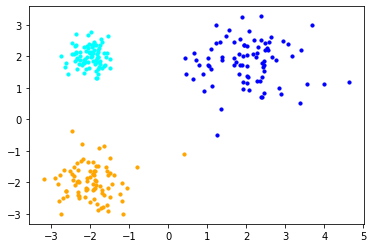
\includegraphics[width=0.7\textwidth]{Images/clusters}
	\caption{Ejemplo de tres clusters claramente distinguibles y separables con densidades distintas.}
	\label{fig:clusters}
\end{figure}



\section{Definiciones formales}

Hasta ahora, se ha dado una interpretación bastante intuitiva acerca de en qué consiste el clustering. Llega el momento de definir formalmente el problema del clustering e introducir su notación. Para tal fin, en toda esta sección nos basaremos en el trabajo realizado en \cite{jose2016automatic}.

\subsection{Notación}

Los siguientes son elementos típicos de un problema de clustering:

\begin{itemize}
	\item Un \emph{objeto}, \emph{patrón} o \emph{instancia} es un dato individual representado por un vector $\textbf{x} = (x_1, x_2,\dots, x_D )^T$, donde $x_i \in \mathbb{R}$ es una \emph{característica} o atributo, y $D$ representa la \emph{dimensionalidad} (el número de características que tienen los objetos). 
	\item Un \emph{conjunto de datos} (o \emph{dataset} en inglés) es una matriz\newline$\textbf{X} = ( \textbf{x}_1, \textbf{x}_2, \dots, \textbf{x}_N )$, donde $\textbf{x}_i \in \mathbb{R}^{D}$ para $i=1,\dots,N$, y $N$ es el número total de objetos en el conjunto de datos.
	\item Un \emph{cluster} puede definirse como una región del espacio que contiene objetos.
	\item Una \emph{solución de clustering} $\textbf{C} = \{c_k | k=1,\dots,K \}$ es un conjunto de clusters disjuntos que particiona al conjunto de datos $\textbf{X}$ en $K$ grupos.
	\item El número de objetos en el cluster $\textbf{c}_k$ es el valor expresado como $n_k = |\textbf{c}_k|$
	\item El \emph{centroide} o \emph{prototipo} del cluster $\textbf{c}_k$ (o prototipo de $\textbf{c}_k$) se expresa como $\textbf{\=c}_k = \frac{1}{n_k}\sum_{\textbf{x}_i \in \textbf{c}_k} \textbf{x}_i$.
	\item El centroide del conjunto de datos \textbf{X} o \emph{centroide global} de \textbf{X} es\newline$\textbf{\=X} = \frac{1}{N} \sum_{\textbf{x}_i \in \textbf{X}} \textbf{x}_i$
	\item Una \emph{medida de distancia} es una métrica usada para cuantificar la proximidad (cercanía o lejanía) entre objetos.
	\item Un \emph{índice de validez} o CVI (\emph{cluster validity index}) usa una medida de distancia para evaluar cuantitativamente una solución de clustering obtenida.
\end{itemize}
\subsection{Tipos de algoritmos de clustering}

El clustering no es un algoritmo en sí, sino el tipo de problema que se pretende resolver, para el cual pueden usarse diferentes técnicas. Tradicionalmente, se han considerado dos tipos de algoritmos para el problema del clustering:

\begin{itemize}
	\item \textbf{Algoritmos de clustering parcicional}: estos algoritmos dividen directamente el conjunto de datos en un determinado número de clusters. De esta forma, un conjunto de datos $\textbf{X}$ es particionado en $K$ grupos (o clusters) disjuntos $\textbf{C} = \{ \textbf{c}_{1},\textbf{c}_{2},\dots,\textbf{c}_{K}\}$, de forma que se cumplan tres condiciones:
	\begin{enumerate}
		\item No puede haber clusters vacíos: $\textbf{c}_i \neq \emptyset,~~~i=1,\dots,K$.
		\item La unión de todos los clusters es igual al conjunto de datos: $\bigcup_{i=1}^{K}\textbf{c}_i =  \textbf{X}$.
		\item Los clusters son disjuntos, es decir, no hay solapamientos: $\textbf{c}_i \cap \textbf{c}_j = \emptyset,~~~~i,j=1,\dots,K~~~ \text{y además} ~~~i \neq j$.
		
		
	\end{enumerate}
	
	El algoritmo de clustering particional más conocido probablemente sea el $k$-means \cite{macqueen1967some}, que funciona asignando cada objeto al cluster cuyo centroide se encuentre más cerca, para posteriormente recalcular los centroides como los promedios de los objetos asociados a los respectivos clusters, de forma que las distancias entre los objetos y los centroides de los clusters a los que están asignados se minimizan.
	
	\item \textbf{Algoritmos de clustering jerárquico}: los algoritmos de este tipo producen como salida una jerarquía de clusters llamada \emph{dendograma}, que representa las agrupaciones anidades de los objetos. Al crear un dendograma, se generan $N$ niveles de clustering, de manera que cada nivel se construye a partir del anterior. De esta forma, no es necesario establecer un número de clusters a priori, puesto que en cada nivel se generan distintos números de clusters. Los dos métodos principales de clustering jerárquico son el aglomerativo y el divisivo.
\end{itemize}




\subsection{Índices de validación}\label{subsct:cvi}

Un índice de validación o CVI (\emph{cluster validity index}) evalúa cómo de buena es una solución (partición) de clustering que ha sido generada por un algoritmo, usando únicamente información inherente al conjunto de datos (es decir, sin tener conocimiento de cuál es la solución óptima, puesto que en aprendizaje no supervisado, en principio, no se sabe cuál es). Un buen índice de validación debería tener un significado intuitivo, debería ser fácil de calcular y debería ser justificable matemáticamente, además de que debería permitir establecer un orden entre las soluciones obtenidas según cómo de buenas son.

Dependiendo del índice que se vaya a emplear para evaluar soluciones, habrá que buscar la solución que maximice o minimice el índice escogido. Por tanto, podemos distinguir entre índices de maximización e índices de minimización.

Son numerosos los índices de validez existentes. A continuación, se listan algunos de los más utilizados:

\begin{itemize}
	\item \textbf{Dispersión intra-grupo} (\emph{within-group scatter}, WGS) \cite{macqueen1967some}. Índice de minimización, también llamado dispersión intra-cluster. Mide la suma de distancias (euclídeas) al cuadrado entre los objetos y los centroides de los clusters a los que pertenecen:
	
	\begin{equation}
		\text{WGS}(\textbf{C}) = \sum_{\textbf{c}_k \in \textbf{C}} \sum_{\textbf{x}_i \in \textbf{c}_k} \text{d}_{\text{e}}^2 (\textbf{x}_i,\textbf{\=c}_k),
	\end{equation}
	
	donde $\text{d}_{\text{e}}(\dots)$ representa la métrica de distancia euclídea entre dos puntos:
	
	\begin{equation}\text{d}_{\text{e}}(\textbf{a},\textbf{b}) = \sqrt{\sum_{i=1}^{n}{(a_i-b_i)^2}}.
	\end{equation}
	

	\item \textbf{Dispersión entre grupos} (\emph{between-group scatter}, BGS) \cite{theodoridis1999pattern}. Índice de maximización. Mide la suma de distancias entre los centroides de los clusters:
	
	\begin{equation}
		\text{BGS}(\textbf{C}) = \sum_{\textbf{c}_k,\textbf{c}_r \in \textbf{C}} \text{d}_{\text{e}} (\textbf{\=c}_k,\textbf{\=c}_r).
	\end{equation}
	
	\item \textbf{Índice de conectividad} (\emph{connectivity index}) \cite{handl2007evolutionary}. Índice de minimización. Mide el grado en el que objetos vecinos han sido asignados al mismo cluster:
	
	\begin{equation}\label{eq:conn}
		\text{Conn}(\textbf{C}) = \sum^{N}_{i=1}\left( \sum^{L}_{j=1} a_{i,n_{ij}} \right),
	\end{equation}
	
	donde
	
	\begin{equation}
	a_{i,n_{ij}} = \begin{cases}
       \frac{1}{j} &\quad\text{si  } \neg \exists \textbf{c}_k : \textbf{x}_i \in \textbf{c}_k \land \textbf{x}_{n_{ij}} \in \textbf{c}_k\\
       0 & \quad\text{en caso contrario}\\
  	\end{cases},
  \end{equation}
	
	donde $n_{ij}$ hace referencia al $j$-ésimo vecino más cercano del $i$-ésimo objeto. Por su parte, $L$ es un parámetro que establece el número de vecinos a tener en cuenta al calcular el índice de conectividad.
	
	Intuitivamente, lo que hace este índice es añadir una penalización cada vez que se detectan objetos vecinos (cercanos) pertenecientes a clusters distintos.
	
	\item \textbf{Índice Calinski-Harabasz} (CH) \cite{calinski1974dendrite}. Índice de maximización. Calinski-Harabasz ofrece una proporción entre la separación y la cohesión  de los clusters. La cohesión se estima como la suma de las distancias entre los objetos y sus respectivos centroides, y la separación se mide como la distancia entre los centroides de los clusters y el centroide global de todo el conjunto de datos:
	
	\begin{equation}
		\text{CH}(\textbf{C}) = \frac{N-K}{K-1} \times \frac{\sum_{\textbf{c}_k \in \textbf{C}} n_k \text{d}_{\text{e}}(\textbf{\=c}_k, \textbf{\=X})}{\sum_{\textbf{c}_k \in \textbf{C}} \sum_{\textbf{x}_i \in \textbf{c}_k} \text{d}_{\text{e}}(\textbf{x}_i, \textbf{\=c}_k)}.
	\end{equation}
	
	\item \textbf{Índice Davies-Bouldin} (DB) \cite{davies1979cluster}. Índice de minimización. En este caso, la cohesión es estimada con la distancia media entre los objetos y sus respectivos centroides, y la separación se calcula con la distancia entre centroides:
	
	\begin{equation}\label{eq:db}
		\text{S}(\textbf{C}) = \frac{1}{K} \sum_{\textbf{c}_k \in \textbf{C}} \max_{\textbf{c}_r \in \textbf{C} \setminus \textbf{c}_k} \left\{\frac{\text{S}(\textbf{c}_k) + \text{S}(\textbf{c}_r)}{\text{d}_{\text{e}}(\textbf{\=c}_k,\textbf{\=c}_r)}\right\},
	\end{equation}
	
	donde
	
	\begin{equation}
	\text{S}(\textbf{c}_k) = \frac{1}{n_k} \sum_{\textbf{x}_i \in \textbf{c}_k} \text{d}_\text{e}(\textbf{x}_i,\textbf{\=c}_k).
	\end{equation}
	
	\item \textbf{Índice Silhouette} (SI) \cite{rousseeuw1987silhouettes}. Índice de maximización. Se trata de una sumatoria normalizada, en en la cual la cohesión se calcula como la suma de las distancias entre los puntos pertenecientes a un mismo cluster, y la separación se basa en la distancia entre los puntos más cercanos pertenecientes a clusters distintos:
	
	\begin{equation}
		\text{SI}(\textbf{C}) = \frac{1}{N} \sum_{\textbf{c}_k \in \textbf{C}} \sum_{\textbf{x}_i \in \textbf{c}_k}
		\frac{\text{b}(\textbf{x}_i,\textbf{c}_k) - \text{a}(\textbf{x}_i,\textbf{c}_k)}{\max\{\text{b}(\textbf{x}_i,\textbf{c}_k),\text{a}(\textbf{x}_i,\textbf{c}_k)\}},
	\end{equation}
	
	donde:
	
	\begin{equation}\text{a}(\textbf{x}_i,\textbf{c}_k) = \frac{1}{n_k} \sum_{\textbf{x}_j \in \textbf{c}_k} \text{d}_{\text{e}}(\textbf{x}_i,\textbf{x}_j),
	\end{equation}
	
	\begin{equation}
	\text{b}(\textbf{x}_i,\textbf{c}_k) = \min_{\textbf{c}_r \in \textbf{C} \setminus \textbf{c}_k} \left\{ \sum_{\textbf{x}_j \in \textbf{c}_r} \text{d}_{\text{e}}(\textbf{x}_i,\textbf{x}_j) \right\}.
	\end{equation}
\end{itemize}
	

\subsection{Clustering como problema de optimización}\label{subsct:optclust}

El problema del clustering puede formularse como un problema de optimización.

Sea $\Omega$ el conjunto de todas las posibles soluciones de clustering (particiones) para un conjunto de datos $\textbf{X}$ dado, y sea $f$ una función objetivo, que puede ser cualquiera de los índices de validez presentados en la sección \ref{subsct:cvi}. Suponiendo que se ha optado por utilizar un índice de validez de minimización, entonces el objetivo del problema de clustering $(\Omega,f)$ consiste en encontrar la solución de clustering óptima $\textbf{C}^{*}$, para la cual

\begin{equation}
	f(\textbf{C}^{*}) = \min\{ f(\textbf{C}) | \textbf{C} \in \Omega \}.
\end{equation}


% ¿Ejemplos uso clustering?

\chapter{El problema del clustering con restricciones}\label{ch:clustering}

El clustering con restricciones es un problema perteneciente al ámbito del aprendizaje semi-supervisado, tal y como se dijo en la introducción. Por ello, es lógico dedicar un apartado que sirva como introducción al aprendizaje semi-supervisdado antres de comenzae a definir y explicar con detalle el clustering con restricciones. Para ello, se ha tomado como referencia principal el capítulo introductorio de \cite{chapelle2006semi}.

\section{Introducción al aprendizaje semi-supervisado}


El aprendizaje semi-supervisado es una de las cuatro modalidades existentes de aprendizaje automático, quizá la menos conocida de ellas. Podría decirse que es un híbrido entre aprendizaje supervisado y aprendizaje no supervisado.

En aprendizaje no supervisado (ver capítulo anterior), se dispone únicamente del conjunto de datos $\textbf{X} = ( \textbf{x}_1, \textbf{x}_2, \dots, \textbf{x}_N )$, compuesto por $N$ muestras o puntos, de forma que el objetivo consiste en encontrar patrones o estructuras en $\textbf{X}$ que puedan ser interesantes. Además del clustering o agrupación, existen otras formas de aprendizaje no supervisado, como la detección de \emph{outliers} o las técnicas de reducción de dimensionalidad.

En aprendizaje supervisado, por su parte, se pretende encontrar una aplicación $\textbf{x} \mapsto y$ dado un conjunto de entrenamiento compuesto por pares $(\textbf{x}_i,y_i)$. En este caso, $y_i$ son las etiquetas de las muestras $\textbf{x}_i$, de forma que, además de $\textbf{X}$, se dispone también del vector de etiquetas $\textbf{y} = (y_1,\dots,y_N)^T$. Nótese que para cada muestra siempre se dispone de una etiqueta. Si las etiquetas adoptan valores continuos ($y_i \in \mathbb{R}$ o $y_i \in \mathbb{R}^p$), la tarea se conoce como regresión, mientras que si adoptan valores discretos (es decir, valores de conjuntos finitos), se conoce como clasificación. Las dos grandes categorías de algoritmos de aprendizaje supervisado son los algoritmos generativos, los cuales pretenden calcular la distribución de problabilidad condicionada $P(\textbf{x}|y)$ para obtener a partir de ella la distribución $P(y|\textbf{x})$, y los algoritmos discriminativos, que en general se limitan a obtener $P(y|\textbf{x})$.

El aprendizaje semi-supervisado es una modalidad a medio camino entre el supervisado y el no supervisado. Efectivamente, se dispone del conjunto de datos sin etiquetas $\textbf{X}$, pero además también se dispone de una cierta cantidad de información supervisada, aunque no para todas las muestras.

En muchas ocasiones, la información supervisada disponible son las etiquetas de algunos puntos de $\textbf{X}$. En tales casos, el conjunto de datos $\textbf{X}$ puede dividirse en dos subconjuntos: por un lado, el conjunto $\textbf{X}_e = (\textbf{x}_0,\dots,\textbf{X}_e)$ para el cual se disponen de las etiquetas $\textbf{y}_e = (y_1,\dots,y_e)$, y por otro lado el conjunto sin etiquetas $\textbf{X}_s = (\textbf{x}_{e+1},\dots,\textbf{X}_{e+s})$.

En otros casos, la información supervisada se da en forma de restricciones. Dichas restricciones indican si algunos ciertos pares de muestras tienen (o no) la misma etiqueta, o si forman parte o no del mismo cluster. A este tipo de aprendizaje semi-supervisado pertenece precisamente el problema que nos ocupa: el clustering con restricciones.

¿Cuándo tiene sentido usar técnicas semi-supervisadas, pudiendo emplear directamente aprendizaje supervisado? En los casos en los que obtener un etiquetado de los datos resulte demasiado costoso, cosa que suele ocurrir a menudo. Por ejemplo: generar conjuntos de datos con grabaciones de voz para un sistema de reconocimiento de voz es una tarea fácil, ya que pueden o bien grabarse expresamente para ello o bien recopilarse de grabaciones previas. Sin embargo, etiquetar ese conjunto de datos con grabaciones no es tan sencillo, pues requiere de alguien que escuche todas esas grabaciones y las transcriba. Otros ejemplos en los que esto también se cumple pueden ser la clasificación de documentos o páginas web, que necesitan que sean leídas por personas, o la clasificación de imágenes, pues igualmente hacen falta personas que vean esas imágenes e indiquen cuál es su contenido.

Dicho esto, ¿podemos esperar un buen rendimiento de las técnicas semi-supervisadas en comparación con las supervisadas? Lo cierto es que sí, pero es necesario asumir algunas hipótesis. Una de ellas, con respecto a la continuidad de la distribución de los datos, consiste en asumir que si dos puntos $\textbf{x}_1$ y $\textbf{x}_2$ en una región con alta densidad de puntos están cerca el uno del otro, entonces sus respectivos valores de salida $y_1$ e $y_2$ también deberían ser cercanos entre ellos. En el caso concreto del clustering, esto se traduce a que, si dos puntos pertenecen a la misma agrupación o cluster (región de alta densidad), entontes lo lógico sería pensar que pertenecen a la misma clase, o que poseen la misma etiqueta. De esta observación se puede inferir que las fronteras de decisión, o sea, los límites entre clusters distintos, deberían transcurrir por regiones de poca densidad, ya que si, de lo contrario, una frontera se situase en una región de alta densidad, un cluster quedaría cortado por dicha frontera. \cite{chapelle2006semi}

\section{Clustering con restricciones}

Esta sección, centrada en describir y formular el problema del clustering con restricciones, tomará como referencia el análisis realizado por Davidson y Basu en \cite{davidson2007survey}.

El clustering con restricciones permite incorporar conocimiento experto sobre el problema en cuestión en forma de restricciones. Existen dos tipos de restricciones a nivel de instancia, definidas por primera vez en \cite{wagstaff2000clustering}:
\begin{itemize}
	\item \textbf{Restricciones \emph{Must-Link}} (ML), denotadas $c_{=}(\textbf{x},\textbf{y})$. Indican que los puntos \textbf{x} e \textbf{y} deben pertenecer a un mismo cluster.
	\item \textbf{Restricciones \emph{Cannot-Link}} (CL), denotadas $c_{\not=}(\textbf{x},\textbf{y})$. Indican que los puntos \textbf{x} e \textbf{y} no pueden pertenecer a un mismo cluster.
\end{itemize}

En particular, las restricciones ML resultan ser una relación de equivalencia entre puntos, por lo que cumplen las propiedades reflexiva, simétrica y transitiva. Esta última es especialmente relevante, ya que permite generar más restricciones ML a partir de las que ya hubiese disponibles:

\begin{observacion}
	\textbf{\emph{Las Restricciones \emph{Must-Link} Son Transitivas.}} Sean $CC_i$ y $CC_j$ componentes conexas, es decir, subgrafos totalmente conectados con restricciones $ML$. Sean $x$ e $y$ dos puntos o instancias en $CC_i$ y $CC_j$ respectivamente. Si $c_{=}(x,y)$ tal que $x \in CC_i,~y \in CC_j$,  entonces $c_{=}(a,b)~\forall a,b: a\in CC_i,~b \in CC_j$ \cite{davidson2007survey} \cite{basu2008constrained}. 
\end{observacion}

Análogamente, aún sin constituir una relación de equivalencia, también pueden inferirse nuevas restricciones CL a partir de otras:

\begin{observacion}
	\textbf{\emph{Las Restricciones \emph{Cannot-Link} Pueden Conllevar Más Restricciones \emph{Cannot-Link} .}} Sean $CC_i$ y $CC_j$ componentes conexas, es decir, subgrafos totalmente conectados con restricciones $ML$. Sean $x$ e $y$ dos puntos o instancias en $CC_i$ y $CC_j$ respectivamente. Si $c_{\not=}(x,y)$ donde $x \in CC_i, y \in CC_j$, entonces $c_{\not=}(a,b)~\forall a,b: a\in CC_i, b \in CC_j$ \cite{davidson2007survey} \cite{basu2008constrained}.
\end{observacion}

Como puede verse, las restricciones ML y CL albergan mucho potencial a pesar de su simpleza. Con ellas es posible encadenar nuevas restricciones, permitiendo aumentar la colección de restricciones de la que se dispone inicialmente.

Además de estas dos propiedades, también existen otras formas de generar nuevas restricciones ML y CL basadas en la distancia:

\begin{itemize}
	\item \textbf{Restricciones Delta} ($\delta$). Para cada punto \textbf{x}, se establece una restricción Must-Link con cada punto \textbf{y} cuya distancia con \textbf{x} sea menor que un cierto valor $\delta$. Con esto, es posible garantizar que los puntos pertenecientes a distintos clusters estén separados por una distancia mayor o igual a $\delta$.
	\item \textbf{Restricciones Épsilon} ($\epsilon$). Para cada punto \textbf{x}, se establece una restricción Must-Link con al menos un punto \textbf{y} cuya distancia con \textbf{x} sea menor o igual a un cierto valor $\epsilon$. Esto permite forzar a que todos los puntos tengan un vecindario de diámetro $\epsilon$.
\end{itemize}

Los métodos que hacen uso de este tipo restricciones que afectan a parejas de instancias (Must-Link, Cannot-Link) se conocen como \textbf{métodos basados en restricciones}. Éstos métodos modifican al algoritmo de clustering en sí para que las restricciones establecidas introduzcan un sesgo en el proceso de búsqueda para poder encontrar la solución correcta. En esencia, existen dos tipos de métodos basados en restricciones:

\begin{figure}
	\centering
	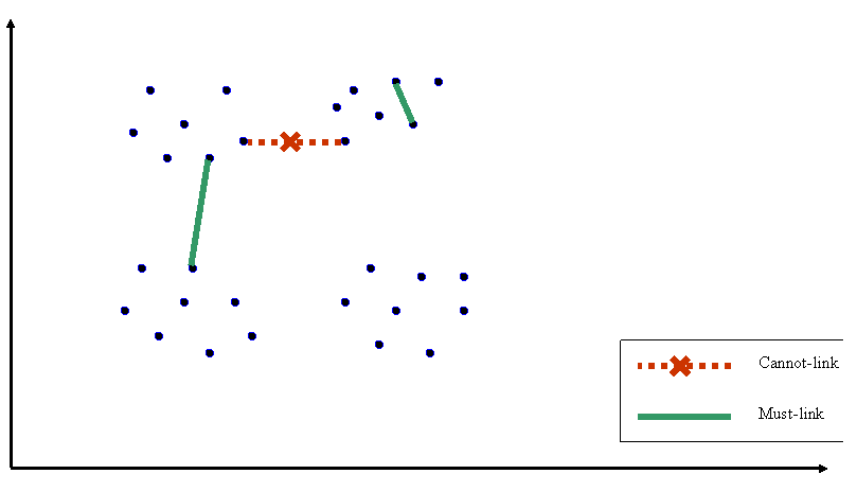
\includegraphics[width=0.75\textwidth]{Images/const_clust}
	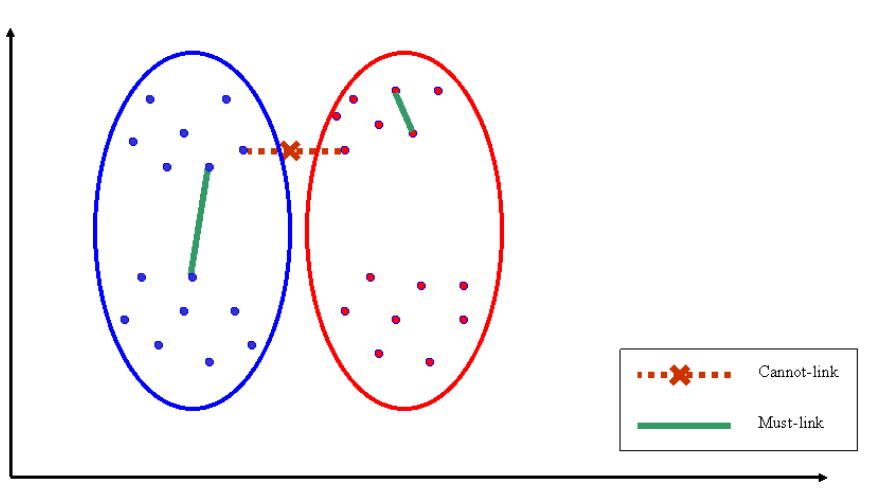
\includegraphics[width=0.75\textwidth]{Images/const_clust_sol}
	\caption[Arriba, un pequeño conjunto de datos con restricciones ML y CL. Abajo, una solución de clustering para ese conjunto de datos que satisface a todas las restricciones.]{Arriba, un pequeño conjunto de datos con restricciones ML y CL. Abajo, una solución de clustering para ese conjunto de datos que satisface a todas las restricciones. \cite{davidson2007survey}}
	\label{fig:const_clust_sol}
\end{figure}


\begin{enumerate}
	\item Aquellos que obligan a que se cumplan las restricciones, de forma que se pretende encontrar la mejor solución que satisfaga a todas ellas \cite{wagstaff2001constrained} \cite{davidson2005hierarchical}.
	\item Aquellos que obligan parcialmente a que se cumplan permitiendo que no todas sean satisfechas, de forma que se busca, por un lado, encontrar la mejor solución de clustering posible, y por otro, maximizar el número de restricciones satisfechas \cite{basu2004active} \cite{segal2003discovering} \cite{davidson2005clustering} \cite{law2005model}.
\end{enumerate}


La otra gran categoría de técnicas de clustering con restricciones está conformada por los llamados \textbf{métodos basados en la distancia}. En ellos, el algoritmo de clustering emplea una medida de distancia \emph{entrenada} o adaptada para que se puedan satisfacer todas las restricciones, en lugar de la distancia euclídea convencional. En este sentido, el espacio es modificado para que se puedan satisfacer las restricciones, de forma que las instancias sujetas a restricciones Must-Link quedan cerca unas de otras, y las restricciones Cannot-Link terminan alejadas entre ellas.

\begin{figure}
	\centering
	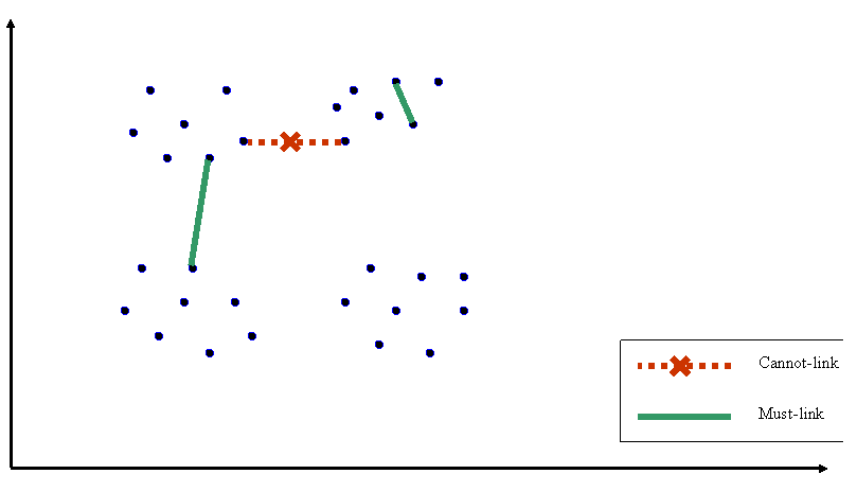
\includegraphics[width=0.75\textwidth]{Images/const_clust}
	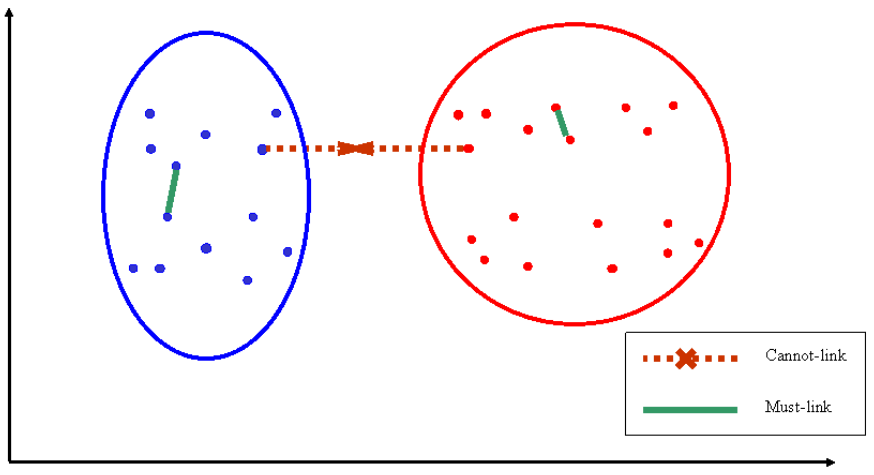
\includegraphics[width=0.75\textwidth]{Images/const_clust_dist}
	\caption[Arriba, un pequeño conjunto de datos con restricciones ML y CL. Abajo, una solución de clustering para ese conjunto de datos después de haber modificado las distancias entre las instancias teniendo en cuenta esas restricciones.]{Arriba, un pequeño conjunto de datos con restricciones ML y CL. Abajo, una solución de clustering para ese conjunto de datos después de haber modificado las distancias entre las instancias teniendo en cuenta esas restricciones. \cite{davidson2007survey}}
	\label{fig:const_clust_dist}
\end{figure}


\subsection{Ventajas e inconvenientes del uso de restricciones en clustering}

Como todo, el clustering con restricciones tiene una serie de beneficios así como de problemas comparado con el clustering básico. En los dos siguientes apartados veremos de cuáles se tratan.

\subsubsection{Ventajas}

Existen dos beneficios principales de la aplicación de restricciones al problema del clustering. La primera, y quizá la más relevante, es la siguiente:

\begin{observacion} 
	\textbf{Las Restricciones Mejoran la Exactitud en el Caso Promedio.} Al hacer el promedio con muchos conjuntos de restricciones distintos, el rendimiento de la predicción de las etiquetas correctas tenderá a aumentar con respecto a no usar restricciones en absoluto. \cite{davidson2007survey}.
	\label{ob:improvement}
\end{observacion}


Se han llevado a cabo numerosos estudios en los que se ha comprobado que esto se cumple. Por poner un ejemplo, en \cite{wagstaff2000clustering} se logró una mejora del 6\%, 10\% y del 20\% para los conjuntos de datos de la UCI Soybean, Pos y Mushroom respectivamente, con tan solo un conjunto de 40 restricciones a nivel de instancia.

El segundo beneficio del uso de restricciones es la posibilidad de \emph{amoldar} la forma geométrica de los clusters resultantes. En \cite{wagstaff2001constrained}, por ejemplo, donde se emplean datos de rutas de coches vía GPS, los clusters que deberían representar las vías no salen con la forma alargada que cabría esperar. Por medio de la implantación de restricciones Cannot-Link entre instancias situadas a más de 4 metros de distancia entre ellas en dirección perpendicular a las carreteras, fue posible corregir los clusters generados para que adoptasen la forma esperada. De esta forma, o con la formación de restricciones $\delta$ y restricciones $\epsilon$, es posible modificar las propiedades geométricas de la forma que mejor convenga.

\subsubsection{Desventajas}

A pesar de haberse demostrado los beneficios del uso de restricciones, existen dos importantes limitaciones que se han de tener en cuenta.

El primer problema es la \textbf{factibilidad}, es decir, el hecho de que sea factible satisfacer todas las restricciones del conjunto de restricciones dado. Si no se emplea un buen método para generar las restricciones, estas pueden contradecirse las unas a las otras, por lo que puede que no exista ninguna solución de clustering que las satisfaga a todas. Por ejemplo, si tenemos dos objetos $\textbf{x}_a$ y $\text{x}_b$, bastaría con definir las restricciones $c_{=}(\textbf{x}_a,\textbf{x}_b)$ y $c_{\not =}(\textbf{x}_a,\textbf{x}_b)$ para tener una contradicción. Una definición más formal de este problema es la siguiente:

\begin{definicion}
 \emph{\textbf{Problema de la factibilidad}:} Dado un conjunto de datos $\textbf{X}$, un conjunto de restricciones $\textbf{R}$, una cota inferior $K_l$ y una cota superior $K_u$, ¿existe una partición de $\textbf{X}$ en $k$ clusters tal que $K_l \leq k \leq K_u$ y que todas las restricciones en $\textbf{R}$ sean satisfechas? \cite{davidson2007survey} \cite{davidson2005clustering}.
\end{definicion}

El problema de la factibilidad es NP-Completo cuando se emplea una conjunción de restricciones Cannot-Link \cite{davidson2007survey}, por lo que el problema de encontrar la mejor solución que satisfaga todas las restricciones puede volverse inviable. Determinar si una única solución satisface todas las restricciones ya es complejo de por sí, pero obtener la mejor solución que las satisfaga a todas lo es aún más.

El otro gran problema del uso de restricciones para el problema del clustering es que \textbf{no todos los conjuntos de restricciones son útiles}, aunque sí sean satisfacibles. Normalmente, se asume que las restricciones son \emph{pistas} que ayudan durante el proceso de búsqueda, puesto que introducen información sobre la solución óptima o verdadera y permiten que, en teoría, sea más fácil obtener una solución similar a la verdadera.

Pensar eso no es descabellado teniendo en cuenta la observación \ref{ob:improvement}. Sin embargo, hay que tener en cuenta que las restricciones mejoran los resultados en el caso promedio, y no todos los conjuntos de restricciones provocarán una mejora. Por ejemplo, en \cite{davidson2006measuring} se demuestra que aún empleando restricciones sin ruido, sin errores y obtenidas directamente de la solución verdadera, es posible que algunos conjuntos de restricciones concretos afecten negativamente al rendimiento. Esto parece ir en contra de lo que suele deducir de otros experimentos, pero el motivo es, de nuevo, que en ellos se promedian los resultados, y en tales casos la observación \ref{ob:improvement} vuelve a cumplirse:

\begin{observacion}
 \emph{\textbf{Conjuntos de Restricciones Concretos Pueden Tener Efectos Adversos}:} Algunos conjuntos de restricciones generados a partir de las etiquetas de la solución verdadera, con la que se evalúan los clusters obtenidos, pueden disminuir la exactitud de la predicción de esas mismas etiquetas \cite{davidson2007survey}.
\end{observacion}


\subsection{Ejemplos de uso}

En \cite{davidson2007survey} se enumeran algunos casos reales de aplicación del clustering con restricciones:
\begin{itemize}
	\item \textbf{Imágenes}: clustering de píxeles para identificación de objetos en la navegación del robot Aibo, mediante el uso de restricciones espaciales (restricciones $\epsilon$ y $\delta$, por ejemplo) [cita]
	\item \textbf{Vídeos}: inclusión de restricciones ML en grupos de píxeles que representan el mismo objeto a lo largo de sucesivos fotogramas [Yan et al. 2004]
	\item \textbf{Biología}: clustering de genes, con restricciones ML para los genes y proteínas que participen en los mismos procesos celulares [Xenarios et al. 2001] [Segal et al. 2003].
	\item \textbf{Audio}: análisis de audio, empleando restricciones para distinguir si dos locutores corresponden a la misma persona o si son diferentes [Bar-Hillel et al. 2003].
	\item \textbf{GPS}: detección de vías y carreteras, empleando restricciones ML en posiciones por las que ha pasado el mismo coche por una carretera, y restricciones CL entre coches situados a más de 4 metros de distancia entre ellas en dirección perpendicular a la de la circulación \cite{wagstaff2001constrained}.
\end{itemize}


\chapter{Los algoritmos evolutivos multiobjetivo}\label{ch:multiobj}

El tipo de algoritmos al que pertenecen aquellos que serán estudiados e implementados en este trabajo son los llamados algoritmos evolutivos multiobjetivo. Para comprenderlos bien, primero será necesario estudiar los dos conceptos clave en los que se basan: la optimización multiobjetivo y los algoritmos evolutivos.

\section{Optimización multiobjetivo}

Antes de comenzar a definir la optimización multiobjetivo, para situar al lector sería lógico hablar brevemente sobre la optimización clásica, es decir, aquella cuyo objetivo consiste en optimizar una única funcion. Eso es justamente lo que se hará a continuación.

\subsection{Problema de optimización de un objetivo}

En los problemas de optimización convencionales, el objetivo consiste en encontrar una solución, dentro del espacio de soluciones posibles, que optimice una única función objetivo. Ya se vio un ejemplo en la sección \ref{subsct:optclust} , donde se formula sin mucho rigor el problema del clustering como un problema de optimización. Una definición general y más formal de los problemas de optimización sería la siguiente:

\begin{definicion}
	
	\emph{\textbf{Problema General de Optimización de un Único Objetivo}:} Un problema de optimización de un único objetivo consiste en minimizar (o maximizar) una función $f(\textbf{x})$ sujeta a $g_i(\textbf{x}) \leq 0$, $i = \{1, \dots, r\}$ y $h_j(\textbf{x})$, $j = \{ 1, \dots, p\}$. Una solución $\textbf{x}$ minimiza (o maximiza) el escalar $f(\textbf{x})$, donde $\textbf{x} \in \Omega$ es un vector $n$-dimensional de variables de decisión $\textbf{x} = (x_1,\dots,x_n)$ de un universo $\Omega$ \cite{coello2007evolutionary}. 
	
\end{definicion}

	
Como se puede ver, $g_i(\textbf{x}) \leq 0$ y $h_j(\textbf{x}) = 0$ representan restricciones que deben cumplirse al optimizar $f(\textbf{x})$. Por su parte el \emph{universo} $\Omega$ es el conjunto que contiene todas las posibles soluciones $\textbf{x}$ que pueden usarse para tanto la función objetivo $f(\textbf{x})$  como las restricciones.
	
El método por el cual se encuentra el óptimo global de una función cualquiera se llama \emph{optimización global}: 
	
\begin{definicion}
 \emph{\textbf{Optimización del Mínimo Global}:} Dada una función $f:\Omega \subseteq \mathbb{R}^n \rightarrow \mathbb{R}$, $\Omega \neq \emptyset$, para $\textbf{x} \in \Omega$ el valor $f^* \equiv f(\textbf{x}^*)$ es el mínimo global si y solo si
 \begin{equation}
 	\forall \textbf{x} \in \Omega:~~f(\textbf{x}^*) \leq f(\textbf{x}),
 \end{equation}
 
 donde $\textbf{x}^*$ es la solución mínima global, $f$ es la función objetivo, y el conjunto $\Omega$ es la región factible de $\textbf{x}$. El objetivo de encontrar la solución o soluciones mínimas globales se llama \textbf{problema de optimización global} \cite{coello2007evolutionary}.
\end{definicion}	



\subsection{Problema de optimización multiobjetivo}\label{sec:mop}

En un principio, puede parecer que la única novedad existente en la optimización multiobjetivo con respecto a la optimización convencional consiste, como su nombre indica, en la optimización de varias una funciones objetivo. Sin embargo, esta diferencia tiene implicaciones que cambian notablemente la forma en la que se trabaja en los problemas de optimización.

La optimización multiobjetivo en general puede definirse de la siguiente forma:

\begin{definicion}
	
	\emph{\textbf{Problema General de Optimización  Multiobjetivo} :} Un problema de optimización multiobjetivo consiste en minimizar (o maximizar) $F(\textbf{x}) = (f_1(\textbf{x}),\dots,f_m(\textbf{x}))$ sujeto a $g_i(\textbf{x}) \leq 0$, $i = \{1, \dots, r\}$ y $h_j(\textbf{x})$, $j = \{ 1, \dots, p\}$. Un problema de optimización minimiza (o maximiza) los componentes de un vector $F(\textbf{x}) \in \mathbb{R}^m$ donde $\textbf{x} \in \Omega$ es un vector de $n$ variables de decisión $\textbf{x} = (x_1, \dots, x_n)$ de un universo $\Omega$ \cite{coello2007evolutionary}.
\end{definicion}

De nuevo, $g_i(\textbf{x}) \leq 0$ y $h_j(\textbf{x}) = 0$ representan las restricciones, y $\Omega$ representa el espacio de soluciones o región factible.

Al optimizar más de una función objetivo, surge un nuevo problema que no se daba cuando se trabaja con una única función objetivo: que no existe una definición consensuada de qué se considera una solución óptima, por lo que resulta difícil comparar unas soluciones con otras \cite{mukhopadhyay2013survey}.


Al ser las funciones objetivo independientes entre ellas, existiendo en ocasiones incluso contradicciones entre ellas, no es posible encontrar siempre una única solución que sea óptima para todas las funciones objetivo a la vez, y por tanto no existe un orden total en el espacio objetivo, sino tan solo un orden parcial \cite{miettinen2012nonlinear}. Por ejemplo, para un espacio objetivo en $\mathbb{R}^2$, podríamos decir que el punto $(1,2)$ es menor que el punto $(3,6)$. Sin embargo, los puntos $(1,3)$ y $(2,1)$ no se podrían comparar tan fácilmente.

Es necesario establecer una forma de determinar qué soluciones son, de alguna forma, mejores que otras. Para ello, introduciremos la terminología de Pareto, que será la que nos permita comparar vectores de valores objetivo $F(\textbf{x})$ y determinar qué soluciones $\textbf{x}$ obtenidas pueden ser útiles, interesantes o válidas para el problema a resolver.

El primer concepto a definir es el de \emph{dominancia de Pareto} o \emph{Pareto-dominancia}, que nos permitirá definir una relación de orden (parcial) entre vectores de valores objetivo:

\begin{definicion}
	\textbf{\emph{Pareto-dominancia}}: un vector $\textbf{u}$ domina al vector $\textbf{v}$ (denotado $\textbf{u} \preceq \textbf{v}$) si, en caso de estar ante un problema de  minimización, $\textbf{u}$ es parcialmente menor que $\textbf{v}$ \cite{jose2016automatic}\cite{coello2007evolutionary}:
	\begin{equation}
	\textbf{u} \preceq \textbf{v} ~\Longleftrightarrow~ \forall i \in \{1,\dots,m\}:~ u_i \leq v_i ~\land~ \exists j \in \{1,\dots,m\}:~ u_j < v_j~.
	\end{equation}
\end{definicion}

Dicho en un lenguaje más natural: el vector $\textbf{u}$ domina al vector $\textbf{v}$ si todos los elementos de $\textbf{u}$ son menores o iguales a los respectivos elementos de $\textbf{v}$, y al menos uno de los elementos de $\textbf{u}$ es estrictamente menor que el elemento correspondiente de $\textbf{v}$. Nótese que esta definición asume que el problema es de minimización. Para los problemas de maximización, bastaría con cambiar los menores o iguales y los menores estrictos, por mayores o iguales y mayores estrictos, respectivamente.

A partir de la dominancia de Pareto, se definen los conceptos de \emph{optimalidad de Pareto} y \emph{conjunto de Pareto}:
\begin{definicion}
	\emph{\textbf{Optimalidad de Pareto} }: Una solución $\textbf{x} \in \Omega$ se dice que es Pareto-óptima con respecto a $\Omega$ si y solo si no existe ninguna otra solución $\textbf{x}'$ tal que $F(\textbf{x}') \preceq F(\textbf{x})$ \cite{coello2007evolutionary} \cite{miettinen2012nonlinear}.
\end{definicion}

\begin{definicion}
	\emph{\textbf{Conjunto Óptimo de Pareto}}:
: Dadas unas funciones objetivo $F(\textbf{x})$, el Conjunto Óptimo de Pareto $\mathcal{P}^*$ se compone de todas las soluciones Pareto-óptimas, es decir, todas las soluciones no dominadas del espacio de soluciones  \cite{coello2007evolutionary}:
	\begin{equation}
		\mathcal{P}^* := \{\textbf{x} \in \Omega ~|~ \neg \exists \textbf{x}' \in \Omega:~F(\textbf{x}') \preceq F(\textbf{x}) \}~.
	\end{equation}
\end{definicion}

El conjunto óptimo de Pareto está formado, en teoría, por las mejores soluciones posibles. Nótese que es todo un \emph{conjunto} de soluciones, y no una única solución óptima. Bien es cierto que, en optimización de un objetivo, pueden obtenerse más de una solución óptima para un problema determinado, pero eso significaría que sus correspondientes valores objetivos $f(\textbf{x})$ serían el mismo. En cambio, en el ámbito de la optimización multiobjetivo se da la particularidad de que se obtienen diversas soluciones óptimas (o en este caso, no dominadas) cuyos respectivos vectores de valores objetivo $F(\textbf{x})$ pueden ser distintos entre ellos, siempre y cuando ninguno de esos vectores domine a otro. Esto pone de manifiesto la complejidad adicional que supone trabajar con más de una función objetivo.

El último concepto relativo a la optimización multiobjetivo que introduciremos es el de \emph{frente de Pareto}:


\begin{definicion}
	\emph{\textbf{Frente de Pareto} \cite{coello2007evolutionary}}: dados unas funciones objetivo $F(\textbf{x})$ y un Conjunto Óptimo de Pareto $\mathcal{P}^*$, el Frente de Pareto $\mathcal{PF}^*$ se define como:
	\begin{equation}
		\mathcal{PF}^* := \{ F(\textbf{x}) ~|~ \textbf{x} \in \mathcal{P}^*\}~.
	\end{equation}
\end{definicion}

El frente de Pareto de un conjunto óptimo $\mathcal{P}^*$ no es sino la imagen del conjunto $\mathcal{P}^*$ en el espacio de valores objetivo, o lo que es lo mismo, es el conjunto de correspondientes vectores objetivo de las soluciones que componen $\mathcal{P}^*$.

¿Cómo puede obtenerse el conjunto óptimo $\mathcal{P}^*$? Un posible método consistiría en generar todas las posibles soluciones de $\Omega$, obtener los vectores de valores objetivos de estas y comprobar cuáles de ellas no son dominadas. Este método, no obstante, no es viable debido al alto número de soluciones del que normalmente se compone $\Omega$ (de hecho, incluso puede tratarse de un conjunto infinito). Como tampoco es fácil, por no decir imposible, obtener una expresión analítica para el frente de Pareto, el procedimiento normal para generarlo consiste en obtener un subconjunto de soluciones de $\Omega$ lo suficientemente grande, para posteriormente obtener sus vectores de valores objetivo y comprobar cuáles de ellos no son dominados \cite{coello2007evolutionary}.

\begin{figure}
	\centering
	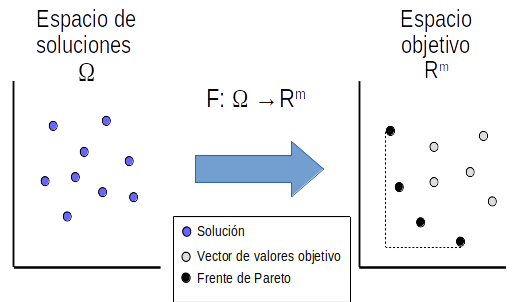
\includegraphics[width=0.9\textwidth]{Images/pareto}
	\caption{Representación gráfica de un frente de Pareto}
	\label{fig:pareto}
\end{figure}

¿Por qué se le llama \emph{frente} al frente de Pareto? Si se dibujan en una gráfica los vectores de valores objetivo $F(\textbf{x})$ de las soluciones $\textbf{x}$ obtenidas, se puede observar que aquellos puntos $F(\textbf{x})$ correspondientes a soluciones no dominadas describen una curva que se sitúa en el límite o frontera del conjunto de puntos obtenidos, y es precisamente en esa frontera donde, en teoría, se encuentran todas las soluciones óptimas, a pesar de que a priori solo se haya generado un subconjunto de ellas. La figura \ref{fig:pareto} ilustra el concepto de frente de Pareto por medio de un sencillo ejemplo.




\section{Algoritmos evolutivos}

Antes de hablar sobre los algoritmos evolutivos multiobjetivo, es lógico dedicar un espacio a los algoritmos evolutivos en general, así como a la clase de algoritmos a los que pertenecen: las metaheurísticas.

\subsection{Metaheurísticas}

Las \emph{metaheurísticas} son una familia de algoritmos de optimización aproximada, muy útiles para resolver problemas de gran dificultad y complejidad puesto que ofrecen soluciones \emph{aceptables} o que pueden considerarse suficientemente buenas en un tiempo razonable. A diferencia de otros algoritmos de optimización, las metaheurísticas no garantizan la optimalidad de las soluciones encontradas \cite{talbi2009metaheuristics}.

Las técnicas metaheurísticas pueden dividirse entre dos grupos principales \cite{jose2016automatic} \cite{talbi2009metaheuristics}:

\begin{itemize}
	\item \textbf{Metaheurísticas de una única solución}. En este tipo de metaheurísticas, una única solución se va mejorando de acuerdo a una función objetivo, de forma que esta solución representa, en muchos casos, un punto que va siguiento una trayectoria en el espacio de soluciones. Ejemplos de esta clase de algoritmos son el enfriamiento simulado (\emph{Simulated Annealing}) \cite{kirkpatrick1983optimization} y la búsqueda tabú (\emph{Tabu Search}) \cite{glover1990tabu}.
	\item \textbf{Metaheurísticas basadas en poblaciones}. Estos algoritmos, como su propio nombre indica, trabajan con toda una población de soluciones. Dicha población es inicializada aleatoriamente, e iterativamente se van generando nuevas poblaciones que son de alguna forma integradas en la población principal usando un cierto criterio de selección. La ventaja de trabajar con toda una población de soluciones en vez de con solo una de ellas es que permite diversificar el proceso de búsqueda en el espacio de soluciones. Ejemplos de metaheurísticas basadas en poblaciones son los algoritmos genéticos o GA (\emph{Genetic Algorithms}) \cite{holland1992adaptation}, la evolución diferencial o DE (\emph{Differential Evolution}) \cite{storn1997differential}, la optimización por nube/enjambre de partículas o PSO (\emph{Particle Swarm Optimization}) \cite{kennedy1995particle} y la optimización por colonia de hormigas o ACO (\emph{Ant Colony Optimization}) \cite{dorigo1996ant}.
\end{itemize}

A su vez, dentro de las metaheurísticas basadas en poblaciones se encuentran los llamados \emph{algoritmos evolutivos}, al que pertenecen, entre otros, los algoritmos genéticos y las técnicas de evolución diferencial.

\subsection{Conceptos básicos de los algoritmos evolutivos}

Los algoritmos evolutivos o EAs (\emph{Evolutionary Algorithms}) tienen en común el hecho de que se basan en la evolución biológica de las especies, de forma que a los individuos de la población de les aplican operadores evolutivos para generar nuevos individuos (llamados \emph{descendientes}) a partir de ellos.
 
Un \emph{individuo} representa una solución codificada al problema que se pretende optimizar, y suele estar representado por cadenas o secuencias de valores, que corresponden al \emph{genotipo} en términos biológicos. El genotipo de un individuo se compone de un cromosoma (o más), y a su vez un \emph{cromosoma} se compone de genes que pueden adoptar determinados valores (\emph{alelos}). De esta forma, cada individuo codifica una serie de parámetros usados como valores de entrada de la función que se desea optimizar. Por último, un conjunto de cromosomas se denomina \emph{población}. \cite{coello2007evolutionary}

Con el fin de generar soluciones cada vez mejores, sobre la población se aplican una serie de operadores inspirados en la biología y la selección natural, llamados \emph{operadores evolutivos}. Los tres operadores usados en los algoritmos evolutivos son: el operador de \emph{cruce} o \emph{recombinación}, el operador de \emph{mutación} y el operador de \emph{selección} \cite{coello2007evolutionary}. A grandes rasgos, el operador de cruce permite generar una o varias soluciones nuevas (descendientes) a partir de una pareja de soluciones de la población (padres). El operador de mutación, por su parte, permite introducir pequeñas alteraciones en las soluciones para, por ejemplo, hacerlas ligeramente diferentes de sus soluciones padres. Finalmente, el operador de selección se utiliza para dar, en general, mayor probabilidad de reproducirse (es decir, de usar el operador de cruce) a los individuos mejores, mientras que análogamente se da menor probabilidad a los peores individuos.

\begin{figure}[h]
	\centering
	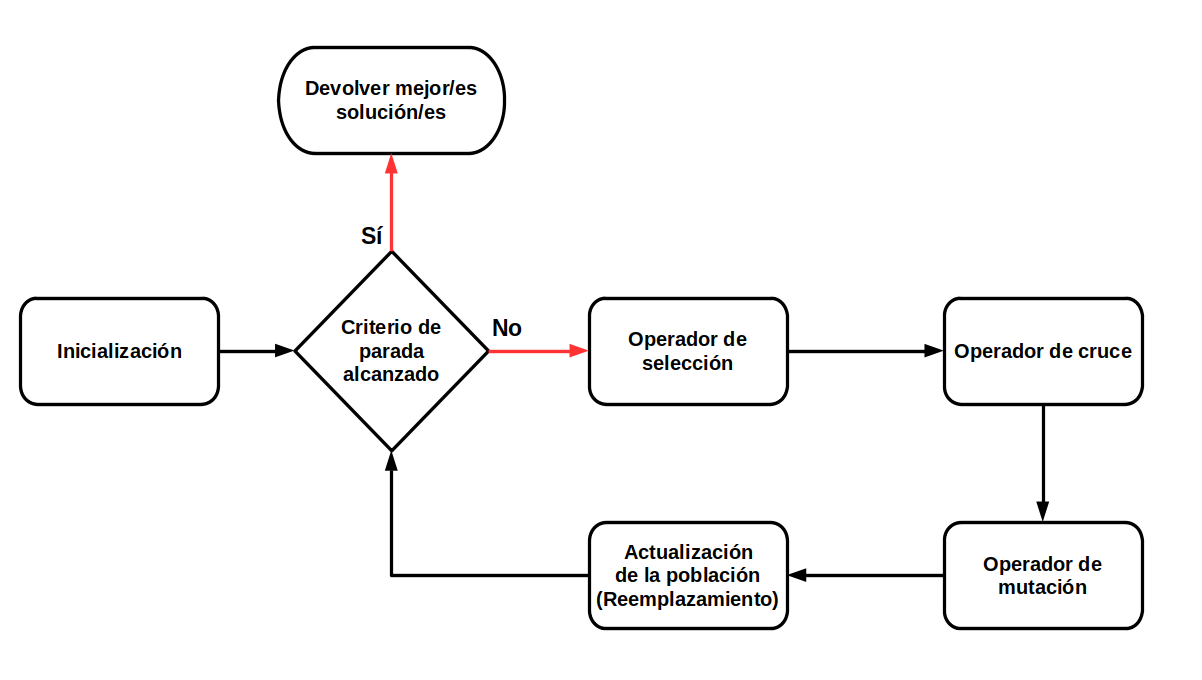
\includegraphics[width=1.0\textwidth]{Images/ga_flowchart}
	\caption[Codificación real.]{Diagrama de flujo de un algoritmo genético, un tipo de algoritmo evolutivo.}
	\label{fig:ga}
\end{figure}


Como ya se sabe, al ser los algoritmos evolutivos un tipo de algoritmos de optimización, estos trabajan con una función objetivo que se pretende optimizar, también llamada en estos casos función de \emph{fitness} \cite{coello2007evolutionary}. La función de \emph{fitness} asignan un valor numérico a las soluciones de conforman la población indicando cómo de buena es cada una de ellas, y es en este valor de bondad en el que se basa el operador de selección para asignar a cada solución su probabilidad de reproducirse.

\subsection{Algoritmos evolutivos para clustering y clustering con restricciones}\label{subsct:evolclust}

Como ya se vió en la sección \ref{subsct:optclust}, el clustering puede formularse como un problema de optimización, y como tal puede ser resuelto con algoritmos evolutivos. Para ello es necesario establecer dos elementos fundamentales: una función objetivo y un esquema de representación o codificación (es decir, la forma en que se codifican los cromosomas que corresponden a las distintas soluciones de la población).

En el caso del clustering clásico, cualquiera de los índices de validación expuestos en la sección \ref{subsct:cvi} puede usarse como función objetivo, mientras que para el clustering con restricciones podría (o debería) usarse un índice o función que tenga en cuenta de alguna forma las restricciones que han sido satisfechas o no. Lo que sí pueden usarse de la misma forma para ambos problemas son los esquemas de representación. Los esquemas de representación para el clustering (y el clustering con restricciones) pueden agruparse en tres clases \cite{jose2016automatic}:

\begin{itemize}
	\item \textbf{Codificación binaria}: Una solución se representa con una secuencia de $N$ dígitos binarios, donde $N=|\textbf{X}|$ es el número de objetos en el conjunto de datos, de forma que cada posición corresponde a un objeto del conjunto de datos. El valor de la $i$-ésima posición será igual a $1$ si el $i$-ésimo objeto del conjunto de datos corresponde a un centroide o prototipo de cluster, mientras que será igual a $0$ en caso contrario.
	
	\begin{figure}[h]
	\centering
	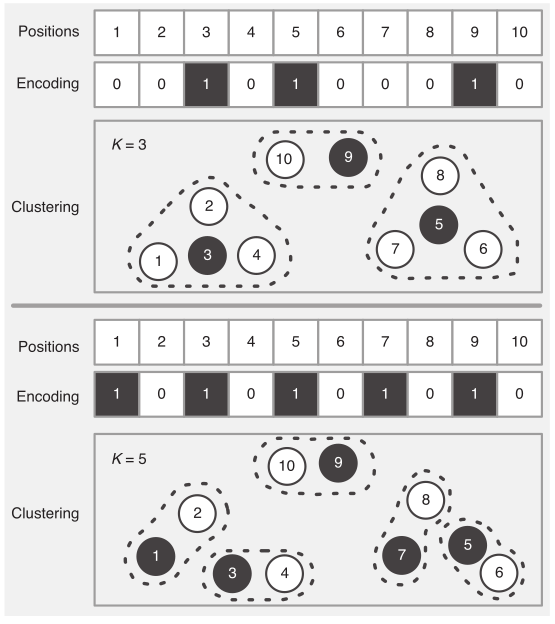
\includegraphics[width=0.8\textwidth]{Images/binary}
	\caption[Codificación binaria para $K=3$ y $K=5$ clusters.]{Codificación binaria para $K=3$ y $K=5$ clusters \cite{jose2016automatic}.}
	\label{fig:binaryencod}
\end{figure}
	
	\item \textbf{Codificación entera}: De forma similar a la codificación binaria, las soluciones se representan con secuencias de $N$ números enteros que codifican todos los objetos del dataset. A su vez, existen dos tipos de esquemas de representación con números enteros:
	\begin{itemize}
		\item \textbf{Representación basada en etiquetas}: En cada posición se guarda un valor entero del conjunto $\{1, \dots, K_{max} \}$ (o del conjunto $\{0, \dots, K_{max}-1 \}$ si se empieza desde el $0$), donde $K_{max}$ es el número máximo de clusters que pueden formarse. De esta forma, si en la posición $i$ del cromosoma aparece el valor $k$, significa que el $i$-ésimo objeto del conjunto de datos $x_i$ pertenece o ha sido asignado al cluster $c_k$.
		
		\begin{figure}[h]
	\centering
	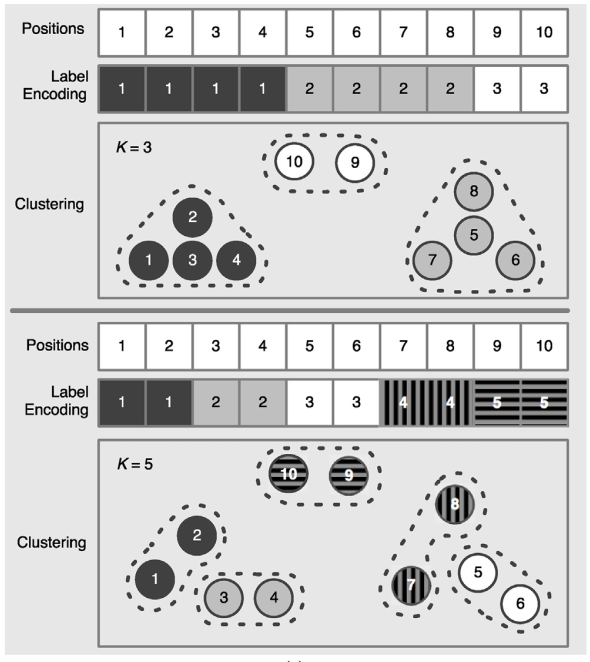
\includegraphics[width=0.8\textwidth]{Images/labelbased}
	\caption[Codificación entera basada en etiquetas.]{Codificación entera basada en etiquetas \cite{jose2016automatic}.}
	\label{fig:labelbasedencod}
\end{figure}
		
		\item \textbf{Representación basada en grafos}: En este esquema el conjunto de datos es tratado como un grafo dirigido. Cada posición de la secuencia puede almacenar valores enteros del conjunto $\{1, \dots, N \}$ (o $\{0, \dots, N-1 \}$), de forma que si en la posición $i$ aparece el valor entero $j$, esto quiere decir que el objeto $x_i$ está conectado al objeto $x_j$. De esta forma, la solución de clustering se construye identificando las distintas partes conexas del grafo, de forma que cada parte conexa del grafo corresponde a un cluster.
	\end{itemize}
	


	\begin{figure}[h]
	\centering
	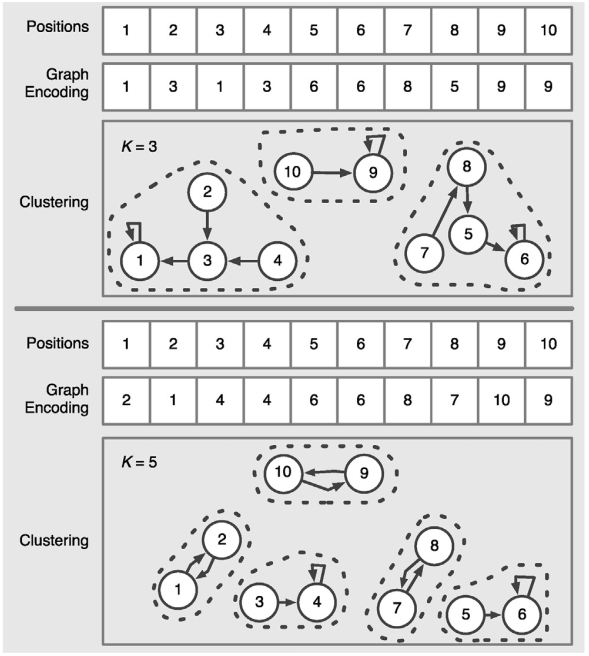
\includegraphics[width=0.8\textwidth]{Images/graphbased}
	\caption[Codificación entera basada en grafos.]{Codificación entera basada en grafos \cite{jose2016automatic}.}
	\label{fig:graphbasedencod}
\end{figure}
	
	\item \textbf{Codificación real}: En este tipo de codificación, los cromosomas representan las localizaciones o coordenadas de los centroides de los clusters en el espacio de características de $D$ dimensiones. Si en el problema a resolver existen $N$ objetos en un espacio $D$-dimensional, los cuales deben ser agrupados en $K$ clusters, entonces los centroides de una solución determinada pueden codificarse con matrices de $D \times K$ valores reales. La codificación real puede ser de tamaño fijo o tamaño variable:
	\begin{itemize}
		\item \textbf{Codificación de longitud fija}: Las soluciones se codifican asumiendo un predeterminado número máximo de clusters $K_{max}$, de forma que todos los cromosomas de la población mantienen la misma longitud de $D \times K_{max}$. Junto a los cromosomas suelen usarse vectores con umbrales de activación para determinar cuáles de esos $K_{max}$ clusters están participando realmente en el agrupamiento.
		
		\item \textbf{Codificación de longitud variable}: Si se tiene un conjunto de $P$ soluciones $\mathcal{C} = \{\textbf{C}_i ~|~ i = 1, \dots, P \}$, la $i$-ésima solución codifica un cierto número de centroides $K_i$. Por tanto, la longitud del cromosoma será variable dependiendo de la solución, teniendo un tamaño de $D × K_i$, aspecto que debe ser tenido en cuenta al hacer uso de los operadores evolutivos.
	\end{itemize}	
\end{itemize}

\begin{figure}
	\centering
	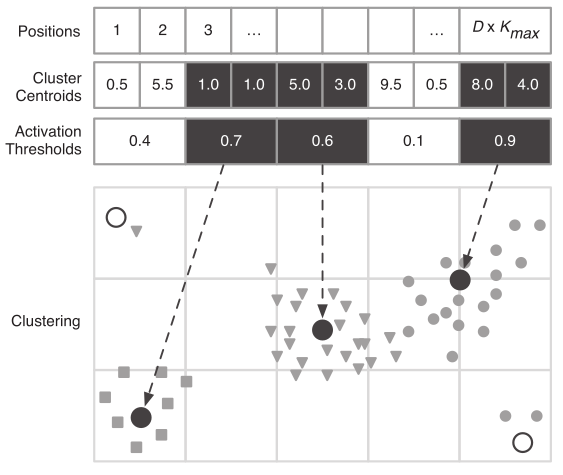
\includegraphics[width=0.8\textwidth]{Images/real}
	\caption[Codificación real.]{Codificación real \cite{jose2016automatic}.}
	\label{fig:realencod}
\end{figure}




Existen diversos ejemplos del uso de algoritmos evolutivos para el problema del clustering y del clustering con restricciones. En \cite{sheikh2008genetic}, por ejemplo, se realiza un análisis sobre el uso de técnicas de clustering basadas en algoritmos genéticos. Por otra parte, en \cite{gonzalez2020dils} se propone un algoritmo evolutivo con búsqueda local, al que llaman DILS (\emph{Dual Iterative Local Search}), en cuya función de \emph{fitness} se suma, por un lado, la sumatoria de distancias al cuadrado entre elementos del mismo cluster, y por otro, un factor de penalización que aumenta cuantas más restricciones son violadas (o sea, no satisfechas). Se trata, como es lógico, de una función de minimización, puesto que una solución es mejor cuanto más cercanos sean los elementos de un mismo cluster y cuantas más restricciones satisfaga.


En definitiva, el uso de algoritmos evolutivos en problemas de clustering, con o sin restricciones, es idóneo dados, por un lado, el hecho de que encontrar la partición óptima en un problema del clustering es de una alta complejidad, y por otro, el hecho de que los algoritmos evolutivos ofrezcan soluciones lo suficientemente buenas en un tiempo aceptable.

\section{Algoritmos evolutivos multiobjetivo}

Los algoritmos evolutivos multiobjetivo o MOEAs (\emph{Multi-Objective Evolutionary Algorithms}) son especialmente adecuados para los problemas de optimización multiobjetivo, ya que al ser algoritmos basados en poblaciones están diseñados para manejar múltiples soluciones durante el proceso de búsqueda \cite{mukhopadhyay2013survey}. 

Una característica relativa a la terminología de Pareto que distingue a los MOEAs de los EAs es el uso de poblaciones adicionales de individuos que no son Pareto-dominados. Muchos MOEAs manejan una población secundaria de soluciones, que al principio está vacía, en la que se van almacenando todas las soluciones no dominadas que se han encontrado hasta el momento. Como la Pareto-dominancia de un vector depende del contexto en el que es evaluado, cada vez que se añade una solución o conjunto de soluciones no dominadas a esa población, las soluciones ya incluidas deben ser comprobadas para asegurarse de que siguen siendo no dominadas. De lo contrario, dichas soluciones son eliminadas de la población secundaria \cite{coello2007evolutionary}.

Tipos de MOEAs

\begin{itemize}
\item A Priori
\item Progresivos
\item Posteriori
\end{itemize}

(Ejemplos de MOEAs)

Uso de MOEAs para clustering (¿clustering con restricciones?)

La ventaja de usar MOEAs para resolver problemas de clustering clásico, al ser multiobjetivos, permiten usar múltiples índices de validación. Pueden usarse al mismo tiempo tanto índices que priorícen la cohesión intra-cluster (p.ej.: minimizar distancias entre las instancias y los centroides de los clusters a los que pertenecen, minimizar distancias entre instancias del mismo cluster, etc.) como índices que se enfoquen en la distancia entre clusters (p.ej.: maximizar distancias entre centroides de los clusters, maximizar distancias entre instancias de clusters distintos), sin que se establezca un orden de prioridad entre ellas.

Además, los MOEAs también son especialmente idóneos para ser usados con problemas de clustering con restricciones, ya que permiten usar como funciones distintas e independientes, por un lado, los índices de validación para clustering clásico para evaluar la calidad de la agrupación obtenida, y por otro, alguna función de insatisfacibilidad para controlar en qué grado se respetan las restricciones impuestas.



\chapter{Algoritmos evolutivos multiobjetivo basados en descomposición}

En este capítulo, será introducida una nueva clase de algoritmos evolutivos que afrontan la optimización objetivo de una forma diferente a los demás: los algoritmos basados en descomposición. Comenzaremos con uno de los más conocidos: el MOEA/D.

%\section{MOEA/D}
\section{Multiobjective Evolutionary Algorithm based on Decomposition}

\emph{Multiobjective Evolutionary Algorithm based on Decomposition}, o por sus siglas MOEA/D, \cite{zhang2007moea} es un algoritmo evolutivo que emplea el concepto de descomposición para resolver problemas de optimización multiobjetivo. La \emph{descomposición} consiste en asociar cada solución de un conjunto óptimo de Pareto a un problema de optimización escalar\footnote{Por <<problema de optimización escalar>>, endiéndase <<problema de optimización con una única función objetivo>>}, de forma que un frente de Pareto pueda ser \emph{descompuesto} en un cierto número de subproblemas de optimización escalar. Para ello, pueden usarse diferentes funciones de agregación que transformen cada vector de valores objetivo en un valor escalar, las cuales se expondrán con detalle más adelante.

La idea de usar descomposición en un MOEA viene dada por el hecho de que la dominancia de Pareto, como ya se vio previamente en la sección \ref{sec:mop}, no define un orden total entre las soluciones en el espacio objetivo, por lo que resulta más difícil en tal caso seleccionar (o descartar) las soluciones que se generan a lo largo del proceso de búsqueda.

\subsection{Funcionamiento general}

MOEAD/D necesita descomponer el problema de optimización multiobjetivo que se pretende resolver, y para ello necesita una función de agregación $g(\textbf{x})$ que tome como entrada una solución de nuestro problema (o sea, un vector \textbf{x}) y devuelva como salida un valor escalar. De esta forma se puede convertir o \emph{descomponer} el problema de optimización multiobjetivo en un cierto número de subproblemas de optimización escalar.

Para tal fin, la función de agregación necesita de vectores de pesos. Cada uno de ellos consiste en un vector de valores no negativos $\boldsymbol\lambda = (\lambda_1,\dots,\lambda_m)^T$ tal que $\sum_{i=1}^m \lambda_i = 1$, de modo que un subproblema de optimización escalar consistiría en encontrar la solución \textbf{x} que optimice la función de agregación $g(\textbf{x} | \boldsymbol\lambda)$ para un $\boldsymbol\lambda$ dado. De esta forma, por cada vector de pesos, existirá un subproblema de optimización escalar, puesto que para cada vector de pesos $\boldsymbol\lambda$ habrá que encontrar la solución $\textbf{x}^*$ que lo optimice. La notación $g(\textbf{x} | \boldsymbol\lambda)$ hace énfasis en el hecho de que $\boldsymbol\lambda$ es un vector de coeficientes, mientras que $\textbf{x}$ es el vector con las variables que se han de optimizar.

En otras palabras, podría decirse que cada $\boldsymbol\lambda$  representa un subproblema, y que por tanto habrá tantos subproblemas escalares como vectores de pesos. Además, lo ideal es que todos ellos estén lo más uniformemente distribuidos para que todo el frente de Pareto quede bien representado al descomponerse.

En MOEA/D se asume que la función de agregación $g(\textbf{x} | \boldsymbol\lambda)$ es continua, y que si dos vectores de pesos $\boldsymbol\lambda^i$ y $\boldsymbol\lambda^j$ son cercanos, sus respectivas soluciones óptimas de $g(\textbf{x} | \boldsymbol\lambda^i)$ y $g(\textbf{x} | \boldsymbol\lambda^j)$ también serán cercanas. Este hecho es importante, porque ayuda a encontrar el $\textbf{x}^*$ óptimo de un determinado vector $\boldsymbol\lambda^i$ a partir de los $\textbf{x}^*$ óptimos de sus vectores más cercanos. Para sacar provecho de ello, se define para cada $\boldsymbol\lambda^i$ un vecindario $B(i) = \{i_1,\dots,i_T\}$, de forma que el conjunto conformado por los vectores $\{\boldsymbol\lambda^{i_1},\dots,\boldsymbol\lambda^{i_T}\}$ representa los $T$ vectores de pesos más cercanos a $\boldsymbol\lambda^i$. De esta forma, como la población se compone de la mejor solución encontrada hasta el momento para cada subproblema, solo las soluciones actuales son aprovechadas para optimizar cada subproblema escalar usando estos vectores de pesos.

Por último, cabe destacar que, como la población se compone de la mejor solución encontrada hasta el momento para cada subproblema, tendremos tantos individuos \textbf{x} como subproblemas. Dicho de otra forma: a cada \textbf{x} de la población de corresponde un vector de pesos $\boldsymbol\lambda$ que lo optimice.

\begin{figure}
	\centering
	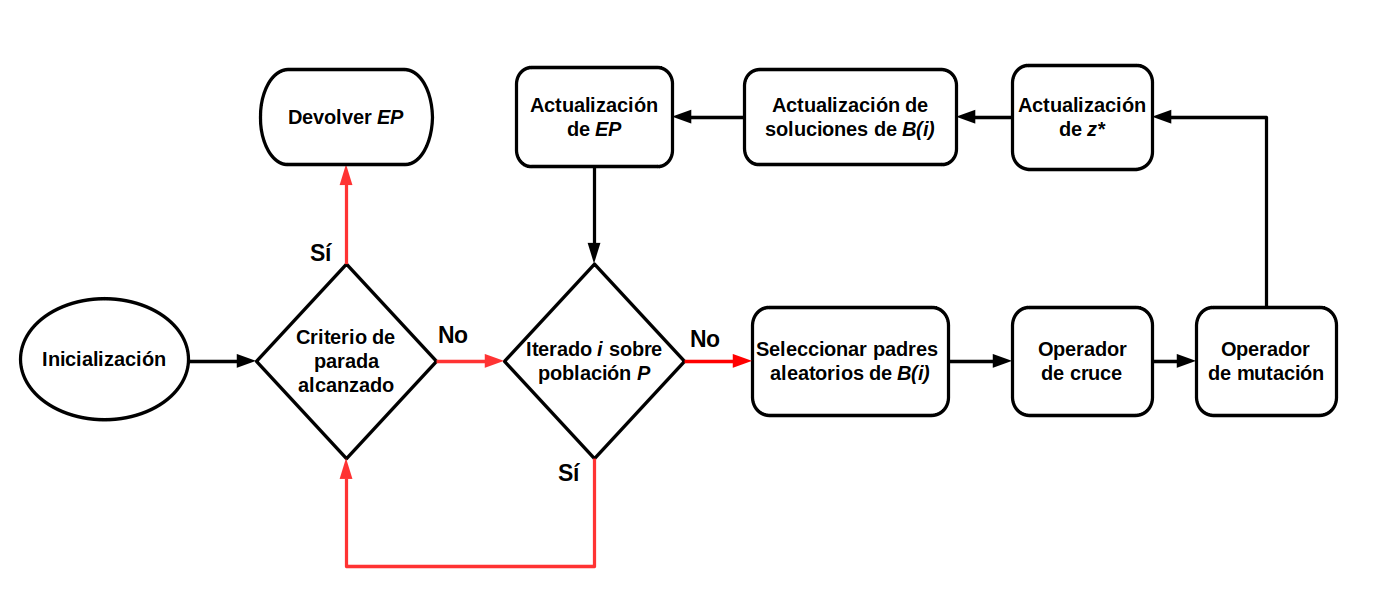
\includegraphics[width=1.1\textwidth]{Images/moead_flowchart}
	\caption{Diagrama de flujo del MOEA/D}
	\label{fig:moeadflow}
\end{figure}

\subsection{Métodos de descomposición}\label{sec:decompmethods}

Las siguientes son algunos métodos de descomposición que pueden emplearse con MOEA/D para generar, por medio de diferentes funciones de agregación, problemas de optimización escalares:

\begin{enumerate}
	\item \textbf{Método de Suma Ponderada} (\emph{Weighted Sum}) .
	
	Sea $\boldsymbol\lambda = \{\lambda_1,\dots,\lambda_m\}$ un vector de pesos no negativos tal que $\sum_{i=1}^m \lambda_i = 1$. La solución óptima para el siguiente problema de optimización:
	
	\begin{equation}
		\max_{\textbf{x} \in \Omega}{~~g^{ws}(\textbf{x} | \boldsymbol\lambda) = \sum^{m}_{i=1} \lambda_i f_i(\textbf{x})}
	\end{equation}
	
	es una solución Pareto-óptima del problema de optimización multiobjetivo a resolver. El conjunto de vectores $\boldsymbol\lambda$ que se utilicen determinará el conjunto de Pareto que se obtenga. Este sencillo enfoque puede resultar útil si el frente de Pareto es convexo (o cóncavo si el problema es de maximización) \cite{miettinen2012nonlinear}.% De lo contrario, es posible que no se encuentren muchas de las soluciones Pareto-óptimas posibles.
	
	\item \textbf{Método de Tchebycheff}.
	
	En este enfoque el problema escalar de optimización es el siguiente:
	
	\begin{equation}\label{eq:tchebycheff}
		\min_{\textbf{x} \in \Omega}{~~g^{te}(\textbf{x} | \boldsymbol\lambda, \textbf{z}^*) = \max_{1 \leq i \leq m}{ \{\lambda_i |f_i(\textbf{x}) - z^*_i|\} }}
	\end{equation}
	
	donde $\textbf{z}^* = (z^*_1,\dots,z^*_m)$ es el punto de referencia o punto ideal, de forma que si nuestro problema es de minimización, entonces $z^*_i = \min_{\textbf{x} \in \Omega}{f_i(\textbf{x})}$. Nótese que se asume que todas las funciones objetivo están acotadas. En caso de no conocer cuál es el punto, puede usarse como aproximación el mínimo de los $f_i(\textbf{x})$ encontrados hasta el momento en el proceso de búsqueda.
	
	Puede demostrarse que el problema de optimización descrito en (\ref{eq:tchebycheff}) siempre tiene al menos una solución óptima, y si esa solución es única, entonces será Pareto-óptima. También se cumple que, para cualquier solución Pareto-óptima $x^*$, siempre existirá un vector de pesos mayores que $0$ para el cual $x^*$ será una solución óptima de (\ref{eq:tchebycheff}) \cite{miettinen2012nonlinear}.
	
	 %La desventaja de este método consiste en que su función de agregación $g^{te}(\textbf{x} | \boldsymbol\lambda, \textbf{z}^*)$ no muestra un comportamiento
	
	\item \textbf{Método de Interseción de Frontera} (\emph{Boundary Intersection}).
	
	
	Normalmente, el frente de Pareto de un problema de optimización objetivo se sitúa en el límite inferior izquierdo o en el límite superior derecho, dependiendo de si el problema es de minimización o maximización respectivamente. Si se dispone de un conjunto de rectas uniformemente distribuidas, los puntos de intersección entre el límite definido por el frente de Pareto y ese conjunto de rectas conforman una buena aproximación del frente de Pareto. Es posible usar este método en MOEA/D usando el punto de referencia $\textbf{z}^*$ y los vectores de pesos $\boldsymbol\lambda$ para construir dichas rectas, de forma que todas las rectas pasen por $\textbf{z}^*$ y tengan como dirección la que determine cada vector $\boldsymbol\lambda$. A partir de ahí, puede generarse el siguiente problema de optimización escalar:
	
	\begin{equation}
	\begin{array}{c}
		\min_{\textbf{x} \in \Omega}{~~g^{bi}(\textbf{x} | \boldsymbol\lambda, \textbf{z}^*) = d} \\
		\text{sujeto a  } ~~F(\textbf{x}) - \textbf{z}^* = d \lambda
		\end{array}.
		\label{eq:bi}
	\end{equation}

	Es preciso aclarar que aquí se asume que el problema de optimización es de minimización. Si, por el contrario, el problema es de maximización, la restricción de igualdad definida en (\ref{eq:bi}) se ha de cambiar por lo siguiente:
	
	
	\begin{equation}
	\textbf{z}^*-F(\textbf{x}) = d \boldsymbol\lambda.
	\end{equation}
	
	  En cualquier caso, esta restricción de igualdad asegura que el vector de valores objetivo $F(\textbf{x})$ siempre se sitúe sobre $L$, la recta con dirección $\boldsymbol\lambda$ (el vector de pesos) y que pasa por el punto $\textbf{z}^*$ (el punto ideal en el espacio objetivo). Esta restricción, sin embargo, resulta difícil de manejar. Para solventar esto, puede utilizarse otro método cuya función de agregación introduzca una penalización, para evitar así la inclusión de restricciones:
	
	\begin{equation}\label{eq:pbi}
		\min_{\textbf{x} \in \Omega}{~~g^{bi}(\textbf{x} | \boldsymbol\lambda, \textbf{z}^*) = d_1 + \theta d_2}
	\end{equation}

	donde, en caso de minimización,
	
	\begin{equation}
	d_1 = \frac{|| (F(\textbf{x}) - \textbf{z}^*)^T \boldsymbol\lambda ||}{||\boldsymbol\lambda||}
	\end{equation}
	\begin{equation}
	d_2 = || F(\textbf{x}) - (\textbf{z}^* + d_1 \boldsymbol\lambda) ||
	\end{equation}
	
	o, si se trata de maximización,

	\begin{equation}
	d_1 = \frac{|| (\textbf{z}^* - F(\textbf{x}))^T \boldsymbol\lambda ||}{||\boldsymbol\lambda||}
	\end{equation}
	
	\begin{equation}d_2 = || F(\textbf{x}) - (\textbf{z}^* - d_1 \boldsymbol\lambda) ||
	\end{equation}
	
	Geométricamente, $d_1$ representa la distancia entre $z^*$ y la proyección de $F(x)$ sobre la recta $L$, mientras que $d_2$ es la distancia entre $F(x)$ y la recta $L$, es decir, la distancia entre  $F(x)$ y su proyección en $L$. Nótese que aquí $d_1$ es el equivalente a $d$ en la expresión \ref{eq:bi}, y $d_2$ es el valor que representa. Por su parte, $\theta > 0$ es un parámetro de penalización que determina cómo de importante es que se minimice $d_2$. Si dicho parámetro $\theta$ es ajustado adecuadamente, las soluciones de ambos métodos (\ref{eq:bi}) y (\ref{eq:pbi}) serán muy similares.
	
	En \cite{zhang2007moea}, este método recibe el nombre de Método de Intersección de Frontera Basado en Penalización o PBI (\emph{Penalty-based Boundary Intersection Method}). Su principal ventaja frente al enfoque de Tchebycheff es que se obtienen soluciones más uniformemente distribuidas, para el mismo conjunto de vectores de pesos. Además, para dos soluciones $\textbf{x}$ e $\textbf{y}$ tales que $\textbf{x} \preceq \textbf{y}$, con el método de Tchebycheff es posible que ocurra que $g^{te}(\textbf{x} | \boldsymbol\lambda, \textbf{z}^*) = g^{te}(\textbf{y} | \boldsymbol\lambda, \textbf{z}^*)$, mientras que es difícil que pase lo mismo con PBI.
	
\begin{figure}[H]
	\centering
	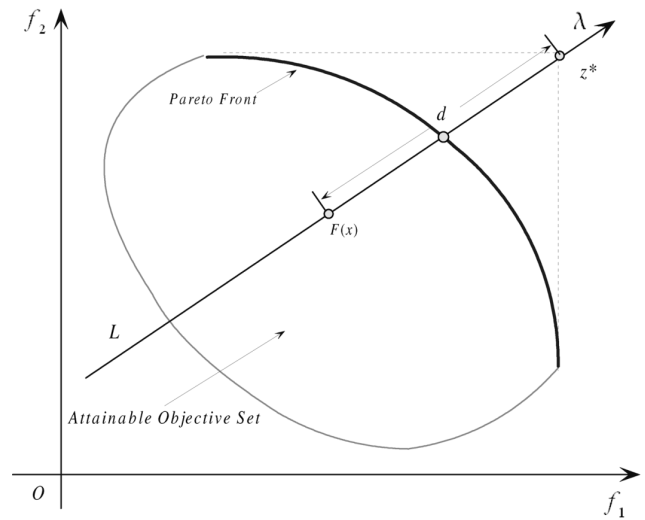
\includegraphics[width=1.0\textwidth]{Images/bi}
	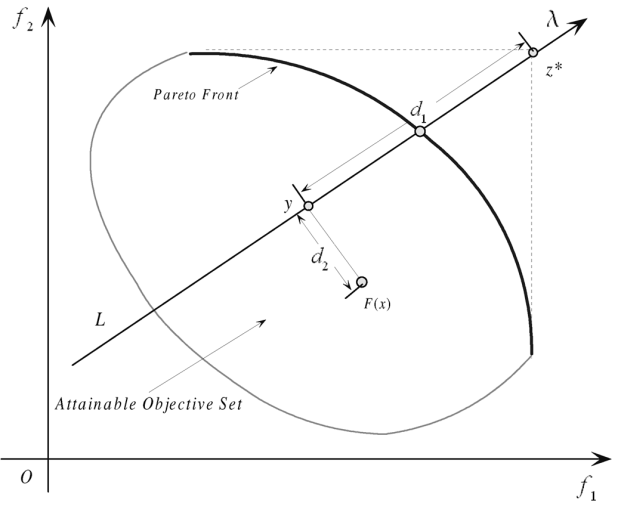
\includegraphics[width=1.0\textwidth]{Images/pbi}
	\caption[Ilustración geométrica de los métodos BI y PBI para un problema de maximización.]{Ilustración geométrica de los métodos BI (arriba) y PBI (abajo) para un problema de maximización \cite{zhang2007moea}.}
	\label{fig:boundaryint}
\end{figure}
	
	Sin embargo, el principal inconveniente del método PBI es el hecho de que $\theta$ sea un parámetro, y como tal debe ser ajustado adecuadamente. Un valor demasiado bajo o demasiado alto provocará que los resultados empeoren.

\end{enumerate}
\newpage



\begin{algorithm}[h]
	\LinesNumbered
	\BlankLine
	\KwIn{Número de subproblemas $N$, tamaño del vecindario de los vectores de pesos $T$, opcionalmente conjunto de vectores de pesos uniformemente distribuidos $\{\lambda_1,\dots,\lambda_N\}$}
	\BlankLine

	\tcc{Inicialización}
	Inicializar población externa $EP = \emptyset$\\
	
	Generar conjunto de vectores de pesos uniformemente distribuidos $\{\lambda_1,\dots,\lambda_N\}$ (si no se ha pasado como entrada)\\
	
	Calcular distancia euclídea entre todos los pares de vectores de pesos. Hayar $B(i) = \{i_1,\dots,i_T\}$ para todo $i\in\{1,\dots,N\}$, de forma que $\boldsymbol\lambda^{i_1},\dots,\boldsymbol\lambda^{i_T}$ son los $T$ vectores más cercanos a $\boldsymbol\lambda^{i}$ \\
	Inicializar, aleatoriamente o de otra forma, la población $P$\\
	
	Obtener valores objetivos de la población $FV$:~~$FV^i = F(\textbf{x}^i)$ para todo $i\in\{1,\dots,N\}$\\
	\BlankLine
	
	\tcc{Actualización}
	\While{criterio de parada no se cumple}{

		\For{$i\in\{1,\dots,N\}$}{
			Elegir aleatoriamente dos valores $l,k \in B(i)$\\
			Generar un descendiente $\textbf{y}$ aplicando el operador de cruce sobre $\textbf{x}^l$ y $\textbf{x}^k$\\
			Aplicar sobre $\textbf{y}$ el operador de mutación. Aplicar opcionalmente mejora o reparación.\\
			
			\BlankLine
			\tcc{Actualizar punto ideal $z$}
			\For{$j\in\{1,\dots,m\}$}{
				
				\If{$f_j(\textbf{y}) \leq z_j$}{
					$z_j = f_j(\textbf{y})$
				}
			}
			\BlankLine
			\tcc{Actualizar soluciones vecinas}
			\For{$j\in B(i)$}{
				\If{$g(\textbf{y} | \boldsymbol\lambda^j) \leq g(\textbf{x}^j | \boldsymbol\lambda^j)$}{
					$\textbf{x}^j = \textbf{y}$,~~~$FV_j = F(\textbf{y})$
				}
			}
			
			\BlankLine
			\tcc{Actualizar población externa}
			Eliminar de $EP$ todas las soluciones dominadas por $F(\textbf{y})$\\
			Añadir $F(\textbf{y})$ a $EP$ si ningún vector de $EP$ domina a $F(\textbf{y})$
		}
	}
	\BlankLine
	
	\KwRet $EP$

	\BlankLine
	\caption{MOEA/D}
	\label{alg:moead}
\end{algorithm}


\section{El framework ADA}

En este apartado se introducirá el esquema usado en este trabajo que introduce el manejo de la multimodalidad en los algoritmos evolutivos multiobjetivo basados en descomposición. Antes de eso, para poner al lector en situación, se hablará brevemente sobre el concepto de multimodalidad y su relación con los MOEAs.

\subsection{Algoritmos evolutivos multimodales multiobjetivo basados en descomposición}

En muchos MOEAs se asume que únicamente la distribución de las soluciones en el espacio objetivo es relevante, dejando en un segundo plano la diversidad en el espacio de soluciones. Sin ir más lejos, un buen ejemplo de esto es el propio MOEA/D, con el cual se puede mantener una buena diversidad en el espacio objetivo si se escoge un método de descomposición adecuado y, sobretodo, si se emplea un conjunto de vectores de pesos que estén uniformemente bien distribuidos \cite{zhang2007moea}. Sin embargo, no existe en MOEA/D ningún mecanismo que mantenga la diversidad en el espacio de soluciones.

Pueden darse situaciones en las que existan diversas soluciones que, aún siendo muy distantes en el espacio de soluciones, son muy próximas o similares en el espacio objetivo, como puede apreciarse en la figura \ref{fig:multimodal}, que ilustra a la perfección el concepto de \emph{multimodalidad}. El hecho de que en un problema existan formas muy distintas de llegar a (casi) la misma solución es algo muy relevante, pues permite elegir entre distintas soluciones de una calidad similar en función de un cierto criterio o preferencia (por ejemplo, que alguna solución sea más fácil de obtener, que una se las soluciones se vuelva inalcanzable o totalmente inviable, etc). Por ello, en ciertos problemas es importante mantener la diversidad en el espacio de soluciones.

Los llamados algoritmos evolutivos multimodales multiobjetivo son MOEAs pensados para problemas en los que se dan precisamente estas circunstancias, los llamados problemas de optimización multiobjetivo multimodales. Su objetivo consiste en encontrar el mayor número de soluciones Pareto-óptimas equivalentes, para lo cual se sirven de mecanismos para manejar múltiples soluciones equivalentes durante su ejecución. Algunos ejemplos de este tipo de algoritmos son el $P_{Q,\epsilon}$-MOEA, el Omni-optimizer y el DIOP, entre otros.


\subsection{ADA: un framework para manejar la multimodalidad}

ADA \cite{tanabe2019framework} es un método propuesto en 2019 para manejar la multimodalidad en los MOEAs basados en descomposición. No se trata de un algoritmo en sí, sino que es un \emph{framework}, es decir, un esquema o marco general que puede aplicarse a distintos algoritmos.

ADA es una generalización de MOEA/D-AD \cite{tanabe2018decomposition}, una versión del MOEA/D capaz de manejar la multimodalidad propuesta por los mismos autores de ADA, con un mecanismo para mantener la diversidad en el espacio basado en el concepto de vecindario de soluciones. Lo cierto es que MOEA/D-AD no es una adaptación trivial del MOEA/D básico, sino que cambia por completo su diseño y funcionamiento.



\subsection{Operadores de ADA}

MOEA/D-AD posee distintos componentes y operadores, cada uno de los cuales cumple un papel fundamental. De hecho, el nombre de MOEA/D-AD viene de MOEA/D \emph{Adition-Deletion}, haciendo alusión a dos de sus componentes: sus operadores de adición y eliminación, respectivamente. ADA posee esos mismos operadores, con la diferencia de que los operadores de MOEA/D-AD son de una forma determinada, mientras que en ADA pueden adoptar distintas formas y variantes, dependiendo de sobre qué algoritmo se esté aplicando.

\subsubsection{Operadores genéticos y de selección}

Como todo algoritmo evolutivo, ADA hace uso de operadores de cruce y mutación para generar nuevas soluciones a partir de las ya existentes. Al igual que en MOEA/D, con ADA puede usarse cualquier operador de cruce clásico, como el operador uniforme o el operador de punto fijo, en caso de usar un esquema de codificación binaria o entera para los cromosomas/individuos de la población, u operadores de cruce como el BLX-$\alpha$ \cite{eshelman1993real} o el SBX \cite{deb1995simulated}, si se usa codificación real. Por supuesto, también pueden usarse operadores de cruce para problemas específicos.

Por su parte, el método de selección de padres de ADA y MOEA/D-AD es de lo más sencillo: mientras que en el MOEA/D original se seleccionaban dos individuos cuyos respectivos vectores de pesos estuviesen en el vecindario del individuo actual $\textbf{x}^i$ (ver líneas 6 y 7 del algoritmo \ref{alg:moead}), en ADA y MOEA/D-AD simplemente se seleccionan dos padres aleatorios de toda la población $P$.

\begin{figure}
	\centering
	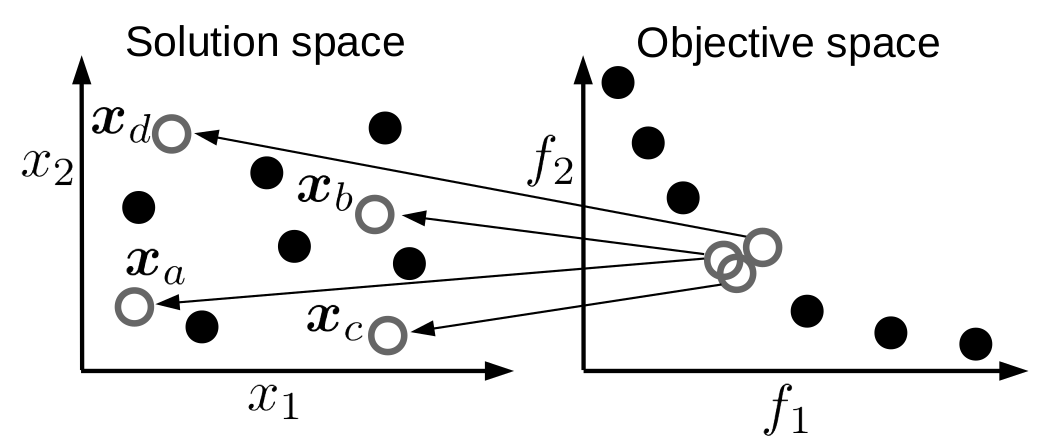
\includegraphics[width=1.0\textwidth]{Images/multimodal}
	\caption[Ilustración del concepto de multimodalidad, en la cual soluciones muy dispares en el espacio de soluciones son casi idénticas en el espacio objetivo.]{Ilustración del concepto de multimodalidad, en la cual soluciones muy dispares en el espacio de soluciones son casi idénticas en el espacio objetivo.\cite{tanabe2019framework}}
	\label{fig:multimodal}
\end{figure}

\subsubsection{Operador de asignación}

En MOEA/D, desde el principio habrá uno y solo un individuo asignado a cada vector de pesos $\boldsymbol\lambda$ (cada uno de los cuales representaba un subproblema), de forma que al individuo $\textbf{x}^i$ le corresponde el subproblema dado por $\boldsymbol\lambda^i$. A lo largo de toda la ejecución, tanto el número de individuos en la población como el número de vectores de pesos se mantiene fijo en $N$, optimizando cada individuo de acuerdo a su correspondiente vector de pesos.

En ADA y MOEA/D-AD no ocurre lo mismo. Mientras que sí se mantienen siempre los mismos vectores de pesos , el tamaño de la población de individuos va cambiando a lo largo del proceso de búsqueda. Además, la forma en la que se asignan las soluciones a los vectores de pesos es diferente: no tiene por qué asignarse el $i$-ésimo individuo $\textbf{x}^i$ al $i$-ésimo vector $\boldsymbol\lambda^i$, si no que ahora $\textbf{x}^i$ se asigna al $j$-ésimo vector $\boldsymbol\lambda^j$, siendo $\boldsymbol\lambda^j$ el vector de pesos que mejor se adapta a $\textbf{x}_i$  bajo un cierto criterio.

Es necesario mantener una estructura que permita saber a qué vector de pesos se ha asignado la solución $\textbf{x}^i$. Así pues, se define el vector $\textbf{a} = (a_1,\dots,a_\mu)$, donde $\mu=|P|$ (recordemos que en ADA y en MOEA/D-AD el tamaño de la población es variable), de forma que si $a_i = j$ entonces al individuo $\textbf{x}^i$ le corresponde el vector $\boldsymbol\lambda^{j}$, y por tanto habrá sido asignado al $j$-ésimo subproblema escalar.

El criterio para asignar individuos a vectores de pesos puede basarse en uno de los métodos de descomposición descritos en la sección \ref{sec:decompmethods}. Si, por ejemplo, se usase el enfoque de Tchebycheff, una solución $\textbf{x}$ se asignaría al $j$-ésimo subproblema, donde:

\begin{equation}
 j = \argmin_{k\in\{1,\dots,N\}}\{g^{te}(\textbf{x}|\boldsymbol\lambda^k)\}
\end{equation}

En MOEA/D-AD, por su parte, se emplea la distancia perpendicular entre el vector normalizado de valores objetivos $F(\textbf{x})$ de una solución $\textbf{x}$, y un vector de pesos $\boldsymbol\lambda$, que no es sino la distancia entre $F(\textbf{x})$ normalizado y su proyección en la recta que pasa por el punto referencia $\textbf{z}$ con la dirección determinada por $\boldsymbol\lambda$ (véase el valor $d_2$ de la fórmula \ref{eq:pbi}).


\subsubsection{Criterio de vecindario}\label{sec:neigh}

Tanto en MOEA/D como en MOEA/D-AD y las variantes de ADA, la diversidad en el espacio objetivo se mantiene mediante la asignación de individuos (soluciones) a los diferentes subproblemas, descrita justo en el apartado anterior. Sin embargo, en lo que se refiere al espacio de soluciones, ningún mecanismo para mantener la diversidad en el espacio de soluciones se emplea en MOEA/D, mientras que en MOEA/D-AD y ADA sí.

La forma de controlar la diversidad en el espacio de soluciones consiste en un criterio de vecindad. Para ello, en \cite{tanabe2019framework} y \cite{tanabe2018decomposition} se propone usar la distancia Euclídea entre soluciones, habiendo normalizado antes las variables de decisión (cromosomas) si en ellas se emplean distintas escalas de valores. De esta forma, puede determinarse para cada solución un vecindario conformado por las $L$ soluciones más cercanas.

Además de este sencillo criterio basado en distancias, con ADA puede usarse cualquier otro criterio de vecindad o de nichos, pero en el estudio preliminar llevado a cabo en \cite{tanabe2019framework} se vió que otros criterios más sofisticados no funcionarion bien.



\subsubsection{Operador de eliminación}

En ADA, el criterio según el cual se descartan las soluciones de la población $P$ es clave, pues ha sido ideado teniendo en mente  la diversidad tanto del espacio de soluciones como la del espacio objetivo.

Sea $\textbf{u}$ una nueva solución generada a partir de dos soluciones padres mediante los operadores genéticos. Se construyen dos conjuntos de soluciones a partir de $\textbf{u}$, a los que llamaremos $Y$ y $Z$, definidos de la siguiente forma:
\begin{equation}
	\begin{array}{c}
		Y = \{ \textbf{x} \in P ~|~ \text{\textbf{x} es vecino de \textbf{u} en el espacio de soluciones} \} \\ 
		Z = \{ \textbf{x} \in P ~|~ \text{\textbf{x} está asignado al mismo subproblema que \textbf{u}} \}
	\end{array}.
\end{equation}


El conjunto $Y$ se basa en el criterio de vecindario que se haya escogido, del cual se habla en el anterior apartado, mientras que $Z$ se basa en el operador de asignación. A partir de estos dos conjuntos, se construye uno tercero, al que llamamos $X$, compuesto por las soluciones que cumplen tanto la condición de $Y$ como la de $Z$: 

\begin{equation}
	X = Y \cap Z
\end{equation}

Posteriormente, se compara la nueva solución $\textbf{u}$ con cada una de las soluciones de $X$. Aquellas soluciones de $X$ que sean peores que $\textbf{u}$ según un cierto criterio serán eliminadas de la población $P$.

¿Por qué se comparan con $\textbf{u}$ solo las soluciones de $X$, y no con las de $Y$ y luego con las de $Z$ por separado? Supongamos que, en un momento dado durante la ejecución de ADA, existe una solución $\textbf{x}'$ tal que $\textbf{x}' \in Z$ y $\textbf{x}' \not\in Y$. Si resultase que $\textbf{x}'$ fuese peor que $\textbf{u}$ y se eliminase de la población $P$, estaríamos perdiendo una solución que aporta diversidad al espacio de soluciónes, ya que $\textbf{u}$ no pertenece al vecindario de $\textbf{u}$. De forma análoga, si $\textbf{x}' \in Y$ pero $\textbf{x}' \not\in Z$, eliminar a $\textbf{x}'$ tampoco tendría sentido aunque fuese, de alguna forma, peor que $\textbf{u}$, porque ni siquiera está asignado al mismo subproblema que $\textbf{u}$, por lo que se perdería una solución que aporta diversidad al espacio objetivo. Por lo tanto, solo eliminando soluciones que pertenezcan a $X$ es posible asegurarse de que no se pierde diversidad ni en el espacio de soluciones ni en el espacio objetivo, porque así se eliminan únicamente soluciones que sean vecinas de $\textbf{u}$ (cercanas a $\textbf{u}$ en espacio de soluciones) y que al mismo tiempo estén asignadas al mismo subproblema que $\textbf{u}$ (cercanas a $\textbf{u}$ en espacio objetivo).

En ADA pueden usarse distintos criterios para determinar si una solución es peor que otra. Si se aplica ADA en algún algoritmo basado en MOEA/D, como el MOEA/D-AGR \cite{wang2015adaptive}, puede usarse cualquiera de los métodos de descomposición listados en la sección \ref{sec:decompmethods}. Si, por ejemplo, se optase por usar el enfoque de Tchebycheff, entonces una solución $\textbf{x}$ sería peor que otra solución $\textbf{y}$ si y solo si $g^{te}(\textbf{y} | \boldsymbol\lambda, \textbf{z}^*) \leq g^{te}(\textbf{x} | \boldsymbol\lambda, \textbf{z}^*)$ para el mismo vector de pesos $\boldsymbol\lambda$. 

\begin{figure}
	\centering
	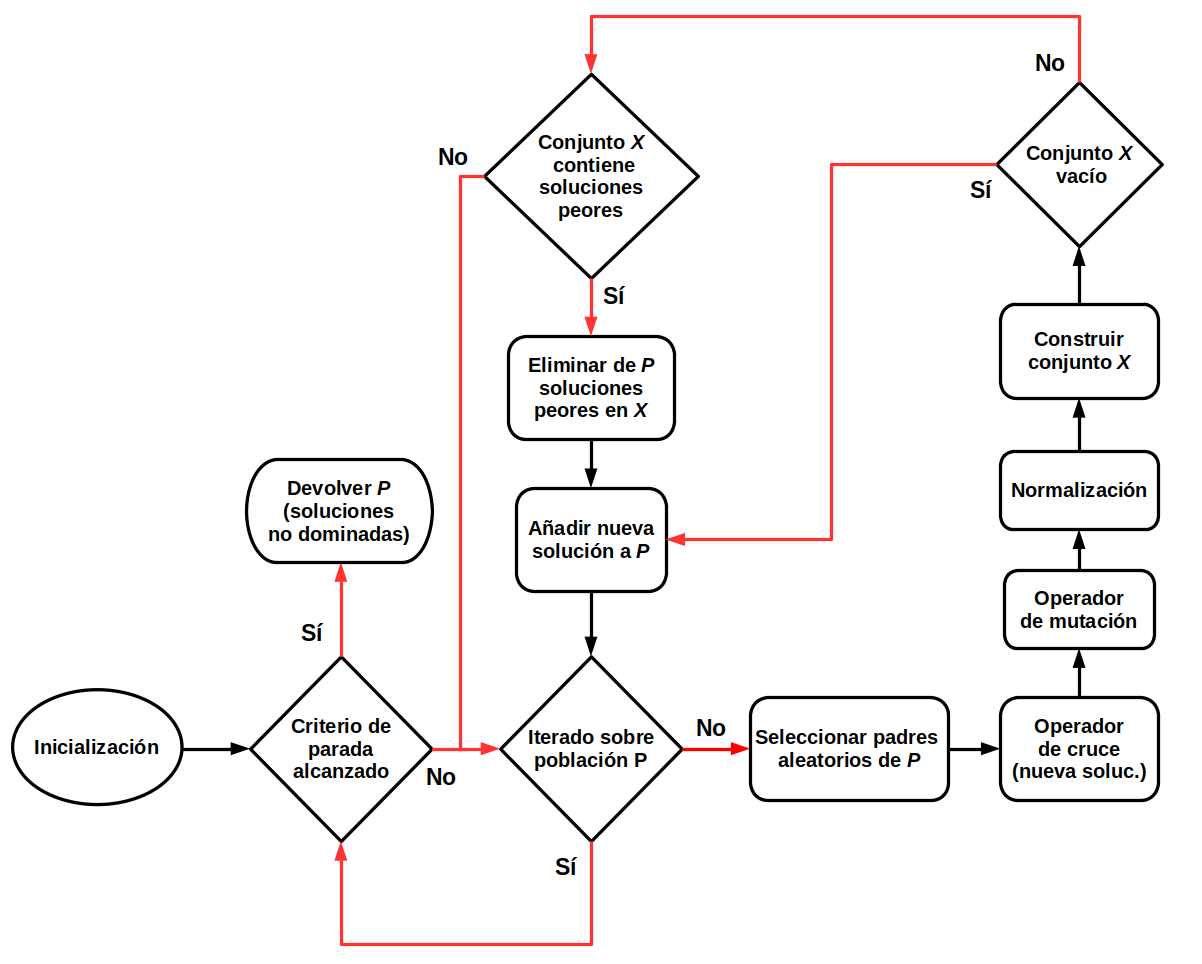
\includegraphics[width=1.1\textwidth]{Images/moead_ada_flowchart}
	\caption{Diagrama de flujo del esquema ADA}
	\label{fig:adaflow}
\end{figure}

\subsubsection{Operador de adición}

Una vez comparada la nueva solución $\textbf{u}$ con todas las soluciones del conjunto $X$ (si las hubiese), y eliminadas aquellas que fuesen peores, llega el momento de decidir qué hacer con $\textbf{u}$: si añadirla a la población $P$ o descartarla. De esto se encargará el operador de adición, el cual añadirá $\textbf{u}$ a la población $P$ si se cumple una de estas dos condiciones:
\begin{enumerate}
	\item Si el conjunto $X$ generado a partir de $\textbf{u}$ no tiene elementos\\($X = \emptyset$).
	\item Si $X$ sí tiene elementos, pero al menos uno de ellos es peor\\que $\textbf{u}$.
\end{enumerate}

¿Por qué se añade $\textbf{u}$ si $X = \emptyset$? Si $X$ no tiene elementos, entonces no existen soluciones en $P$ que sean vecinas de $\textbf{u}$ en el espacio de soluciones y que al mismo tiempo estén asignadas al mismo subproblema (puede que existan soluciones que cumplan una condición u otra, pero no ambas a la vez, ya que en tal caso formarían parte de $X$). Por tanto, $\textbf{u}$ es una solución que aporta diversidad, ya sea al espacio de soluciones, al espacio objetivo, o a ambos, por lo que tiene sentido añadirla a la población $P$ aunque esta ya contenga soluciones que sean mejores que $\textbf{u}$.

\begin{figure}[h]
	\centering
	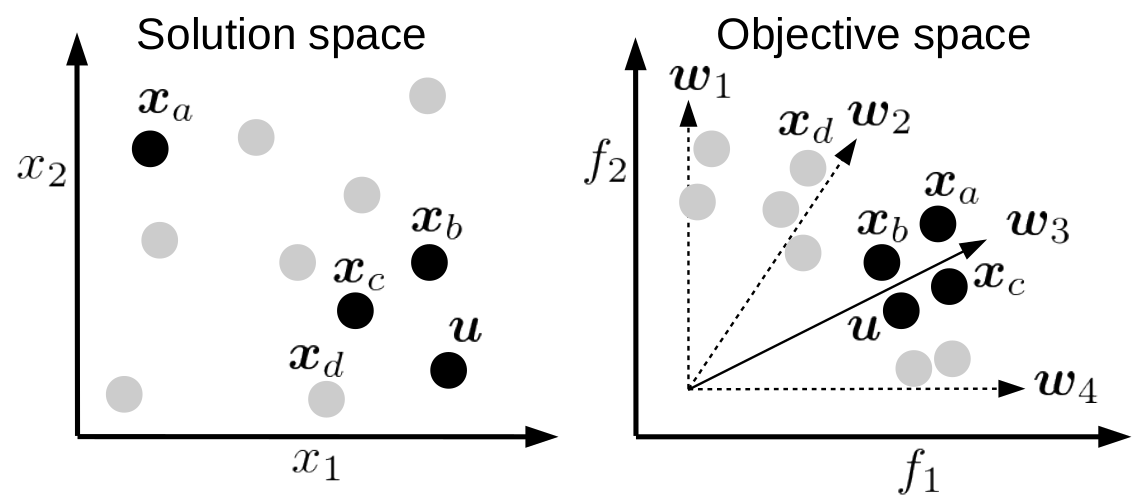
\includegraphics[width=1.0\textwidth]{Images/same_subproblem}
	\caption[Ejemplo que ilustra cómo las soluciones asignadas al mismo subproblema/vector de pesos son cercanas entre sí en el espacio objetivo.]{Ejemplo que ilustra cómo las soluciones asignadas al mismo subproblema/vector de pesos son cercanas entre sí en el espacio objetivo. \cite{tanabe2019framework}}
	\label{fig:assigsubproblem}
\end{figure}


¿Por qué, si $X \not = \emptyset$, $\textbf{u}$ se añade solo si alguna de las soluciones de $X$ es peor que $\textbf{u}$? Porque al ser vecinas de $\textbf{u}$ y estar asignadas al mismo subproblema, no se perderá diversidad si son sustituidas por $\textbf{u}$. Por tanto, si se han eliminado de $P$ soluciones que formaban parte de $X$ por ser peores que $\textbf{u}$, lo lógico es añadir a la propia $\textbf{u}$ a $P$ para reemplazarlas.



\newpage

\begin{algorithm}
	\LinesNumbered
	\BlankLine
	\KwIn{Número de subproblemas $N$, proporción de vecindario $\tau$}
	\BlankLine
	\tcc{Inicialización}
	Inicializar población externa $EP = \emptyset$\\
	
	Generar conjunto de vectores de pesos $\{\lambda_1,\dots,\lambda_N\}$\\
	
	Inicializar, aleatoriamente o de otra forma, la población $P$\\
	
	Obtener $FV$:~~$FV^i = F(\textbf{x}^i)$ para todo $i\in\{1,\dots,N\}$\\
	
	Inicializar problemas asignados $\textbf{a} = (a_1, \dots, a_N)$
	
	\tcc{Op. Asignación}
	\For{$i\in\{1,\dots,N\}$}{
		Encontrar $j$-ésimo subproblema que mejor se adapte a $\textbf{x}^i$\\
		$a_i = j$\\
	}
	\While{criterio de parada no se cumple}{
		\tcc{Tamaño de población y vecindario}
		$\mu = |P|$,  $T = \mu \cdot \tau$\\
		
		\BlankLine
		\tcc{Selección de padres y op. genéticos}
		Seleccionar dos valores aleatorios $a,b \in \{1,\dots,\mu\}$ \\
		Generar un descendiente $\textbf{u}$ aplicando el operador de cruce sobre $\textbf{x}^a$ y $\textbf{x}^b$\\
		\BlankLine
		Aplicar sobre $\textbf{u}$ el operador de mutación. Aplicar opcionalmente mejora o reparación.\\
		Normalizar los vectores de valores objetivos $F(\textbf{u})$ y $FV$\\
		Encontrar $j$-ésimo subproblema que mejor se adapte a $\textbf{u}$\\
		Generar vecindario de $\textbf{u}$ ($T$ soluciones más cercanas)
		$X = \{\textbf{x} \in P ~|~ \textbf{x} \text{ está asignado al subproblema } j \land \textbf{x} \text{ está en el vecindario de \textbf{u}} \}$
		\BlankLine
		% SEPARAR AQUÍ
		\tcc{Op. Eliminación}
		$b^{\text{ ganador}} = FALSE$\\
		$b^{\text{ explorador}} = FALSE$\\
		
		\If{$X = \emptyset$}{
			$b^{\text{ explorador}} = TRUE$\\
		}
		
		\For{$\textbf{x} \in X$}{
			\If{$\textbf{x}$ es peor que $\textbf{u}$}{
					$P = P \setminus \{\textbf{x}\}$\\
					$b^{\text{ ganador}} = TRUE$\\
				}
		}
		
		\BlankLine
		\tcc{Op. Adición}
		\If{$b^{\text{ explorador}} \lor b^{\text{ ganador}}$}{
			$P = P \cup \{\textbf{u}\}$\\
			Añadir $j$ al final de $\textbf{a}$\\
		}
		
	}
	\BlankLine
	\KwRet $P$
	\BlankLine
	\caption{El framework ADA}
	\label{alg:ada}
\end{algorithm}
\newpage




 
 \begin{algorithm}
	\LinesNumbered
	\BlankLine
	\KwIn{Número de subproblemas $N$, tamaño del vecindario de los vectores de pesos $T$, opcionalmente conjunto de vectores de pesos uniformemente distribuidos $\{\lambda_1,\dots,\lambda_N\}$}
	\KwOut{Población externa $EP$}
	\BlankLine
	Adicion\\
	Eliminacion
	\BlankLine
	
	\KwRet $EP$

	\BlankLine
	\caption{MOEA/D-AD}
	\label{alg:moeadad}
\end{algorithm}


\part{Experimentación}
\chapter{Metodología}\label{ch:methodology}

Como se anticipó en el capítulo introductorio, la segunda parte de este trabajo gira en torno a la experimentación realizada. En este capítulo en concreto se explicarán todos los datos, parámetros, variantes y medidas de rendimiento elegidos para los experimentos.

\section{Esquema de codificación}

Para aplicar ADA al problema del clustering con restricciones, se empleará un esquema de \textbf{representación entera basada en etiquetas}. Existen dos principales motivos por los que la representación basada en etiquetas es una buena opción para el clustering y el clustering con restricciones:

\begin{enumerate}
 \item La representación basada en etiquetas permite la \textbf{formación de clusters con cualquier forma}. En general, los esquemas de codificación entera, tanto la basada en etiquetas como la basada en grafos, son capaces de generar clusters no convexos, a diferencia de los esquemas de representación binarios y de representación real, los cuales, al basarse en la cercanía de cada instancia a los centroides, únicamente forman clusters convexos.
 
 \item La representación basada en etiquetas es la \textbf{forma de representación más directa}. Este esquema de representación es la única que no requiere de un proceso de \emph{decodificación} a posteriori para averiguar a qué cluster pertenece cada punto o instancia, puesto que esa información ya queda representada de forma explícita. Por tanto, será más rápido evaluar una solución (es decir, obtener sus valores objetivo).
 
 En el caso de la representación entera basada en grafos, habría que decodificar los grafos dirigidos que representan las soluciones, viendo en cada caso a qué otras instancias está conectada cada una para identificar los componentes conexos, cada uno de los cuales representaría un cluster distinto.
 
 Por su parte, en la representación binaria y la representación real, para saber a qué cluster pertenece cada instancia, hace falta comprobar cuál de los $k$ centroides es el más cercano a ella.
 
 En definitiva, al decodificar una solución de alguno de los esquemas de representación que así lo requieren, el resultado obtenido es un vector con las etiquetas que indican a qué cluster pertenece cada objeto o instancia, por lo que si se opta desde el principio por la representación basada en etiquetas no haría falta aplicar dicho proceso de decodificación a las soluciones.
\end{enumerate}

\section{Funciones objetivo a optimizar}

Como ya se dijo, en este trabajo se pretende enfocar el problema de clustering con restricciones como un problema de optimización. Así pues, se emplearán tres funciones objetivo: dos de ellas corresponden a índices de validación de los vistos en la sección \ref{subsct:cvi}, y una tercera mide el grado en que se satisfacen (o violan) las restricciones.

Los dos índices de validación elegidos son el \textbf{índice Davies-Bouldin} y el \textbf{índice de conectividad}, definidos según las expresiones (\ref{eq:db}) y (\ref{eq:conn}), respectivamente. El índice Davies-Bouldin consiste en un valor que tiene en cuenta tanto la cohesión de cada cluster como la separación de cada cluster. Por su parte, el índice de conectividad penaliza a las instancias cuyas instancias vecinas (o sea, las más cercanas) pertenezcan a clusters distintos, favoreciendo que los elementos de distintos clusters se mantengan a una cierta distancia y contribuyendo, de esta forma, a la separación entre clusters. En definitiva, estos dos índices juntos constituyen una buena forma de estimar (y mejorar) la calidad de una solución de clustering.

Por su parte, la tercera función objetivo, que es la que tiene en cuenta las restricciones, consiste simplemente en el \textbf{número de restricciones insatisfechas}, es decir, la suma de restricciones, tanto Must-Link como Cannot-Link, que no han sido satisfechas:

\begin{equation}
	Insatis(\textbf{C}, C_{=}, C_{\not=}) = Insatis(\textbf{C},C_{=}) + Insatis(\textbf{C},C_{\not=}),
\end{equation}


donde $\textbf{C}$ es una solución de clustering, y $C_{=}$ y $C_{\not=}$ son los conjuntos de restricciones ML y CL, respectivamente.

Las tres funciones objetivo son de minimización, y además están acotadas inferiormente ya que el valor mínimo de todas ellas es de $0$. Esto último será especialmente relevante a la hora de definir el vector de referencia $\textbf{z}^*$, usado en los métodos de descomposición de Tchebycheff, BI y PBI.

\section{Variantes de ADA}

Este trabajo tiene como fin comprobar cómo funciona ADA con el problema del clustering con restricciones. Para ello, se aplicará ADA al algoritmo MOEA/D y se introducirán pequeñas modificaciones hasta crear un total de $8$ variantes de ADA distintas, las cuales serán comparadas entre ellas. Las variantes con las que se experimentará son las siguientes:

\begin{itemize}
	\item $\textbf{MOEA/D-ADA}$: la versión más básica que se probará. Tal y como ocurre en el algoritmo MOEA/D-AGR-ADA, la forma de comprobar si una solución es peor que otra, así como la asignación de las soluciones a subproblemas, se hará con el método de Tchebycheff. No se aplicará normalización a los valores objetivo de las soluviones.
	\item $\textbf{MOEA/D-ADA}_{Norm}$: esta versión es exactamente igual a la anterior, con la única diferencia de que los valores objetivo se normalizan, tal y como se especifica en el planteamiento original de ADA, con el fin de que las distintas en las que se mueven las funciones objetivo no influyan. La normalización consiste en un escalado simple que utiliza el punto ideal $\textbf{z}^*$ para que los valores objetivo pasen al rango $[0,1]$. Suponiendo minimización:
	\begin{equation}
	f'_i(\textbf{x}) = \frac{f'_i(\textbf{x})-\textbf{z}^*_{\text{peor}}}{\textbf{z}^*-\textbf{z}^*_{\text{peor}}},
	\end{equation}
	donde $\textbf{z}^*_{\text{peor}}$ representa el punto contrario a $\textbf{z}^*$, es decir, el punto con los máximos valores objetivo encontrados hasta el momento. 
	\item $\textbf{MOEA/D-ADA-PD}$: partiendo de la versión básica, $\text{MOEA/D-ADA}$, en la asignación de subproblemas se empleará, en lugar del método de Tchebycheff, la distancia perpendicular entre la solución y el vector de pesos, tomando la idea del algoritmo MOEA/D-AD.
	\item $\textbf{MOEA/D-ADA-PD}_{Norm~A}$: idéntica a $\textbf{MOEA/D-ADA-PD}$, pero con normalización de valores objetivo
	\item $\textbf{MOEA/D-ADA-PD}_{Norm~B}$:
	\item $\textbf{MOEA/D-ADA-PD-SSPS}$:
	\item $\textbf{MOEA/D-ADA-KM}$: versión idéntica a $\text{MOEA/D-ADA}$, pero aplicando el algoritmo de $k$-medias al 20\% de la población inicial. Esto puede ser beneficioso si en los conjuntos de datos con los que se vayan a usar estos algoritmos predominan los clusters convexos, pero puede no ser el caso. De hecho, este es uno de los motivos por los que se utilizan restricciones: para evitar la tendencia a generar clusters convexos o hiperesféricos, corrigiendo su forma según la información disponible sobre la solución óptima.
	\item $\textbf{MOEA/D-ADA-PD-KM}$: de forma análoga a la versión anterior, esta versión es como $\text{MOEA/D-ADA-PD}$ pero aplicando $k$-medias al 20\% de la población tras la inicialización.
\end{itemize}

%\newgeometry{left=1.0cm}
\begin{table}[h]
\centering
\caption{Variantes de ADA comparadas}
\resizebox{1.3\textwidth}{!}{
	\begin{tabular}{|c|c|c|c|c|}
	\hline
	Variante & Normalización & Op. selección & Op. asignación & Inic. con $k$-medias\\
	\hline
	$\text{MOEA/D-ADA}$ & No & Padres aleatorios& Tchebycheff & No\\
	$\text{MOEA/D-ADA}_{Norm}$ & Sí & Padres aleatorios  & Tchebycheff & No\\
	$\text{MOEA/D-ADA-PD}$ & No & Padres aleatorios & Dist. perpendicular & No\\
	$\text{MOEA/D-ADA-PD}_{Norm~A}$ & Sí & Padres aleatorios & Dist. perpendicular & No\\
	$\text{MOEA/D-ADA-PD}_{Norm~B}$ & Solo en op. asign. & Padres aleatorios de $P$ &  Dist. perpendicular & No\\

	$\text{MOEA/D-ADA-PD-SSPS}$ & No & Padres aleat. asignados al mismo subprob. & Tchebycheff & No\\
	$\text{MOEA/D-ADA-KM}$ & No & Padres aleatorios& Tchebycheff & 20\% población\\
	$\text{MOEA/D-ADA-PD-KM}$ & No & Padres aleatorios de& Dist. perpendicular & 20\% población\\
	\hline
	\end{tabular}
}
\label{tab:constraints}
\end{table}
%\restoregeometry

\subsection{Inclusión de población externa}

En todas las variantes se ha incluido un mecanismo de población externa ($EP$) que no existía en ADA. Obtener soluciones no dominadas de $P$ da como resultado demasiado pocas soluciones, con lo cual es menos probable terminar con soluciones tan buenas que como si se tuviese una población externa que guarde todas las soluciones no dominadas obtenidas hasta el momento a lo largo de la ejecución del algoritmo. Puede que se pierda algo de diversidad (en espacio objetivo y espacio de soluciones) porque puede que existan soluciones que durante el proceso de búsqueda de ADA fuesen eliminadas por ser peores que una solución que fuese mejor según el método de Tchebycheff, y que además estas estuviesen en su vecindario y asignadas al mismo subproblema. Sin embargo, tras los estudios preliminares, se puede decir que se consiguen mejores resultados en general manteniendo las soluciones no dominadas en una población externa.

\subsection{Métrica de distancia en el espacio de soluciones}

Algo a tener en cuenta a la hora de aplicar ADA a un problema de optimización es el criterio de vecindario de soluciones de ADA (ver sección \ref{sec:neigh}). En todas las variantes que se han usado aquí, el criterio de vecindario usado para construir el conjunto $X$ se basa en la \textbf{distancia euclídea}. Bien es cierto que en \cite{tanabe2019framework} y en \cite{tanabe2018decomposition} se emplea la distancia euclídea normalizada, es decir, la distancia euclídea entre dos puntos habiendo normalizado antes ambos puntos para que sus valores/características/cromosomas adopten únicamente valores entre 0 y 1. Sin embargo, en nuestro caso no es necesario normalizar las soluciones, puesto que, al haber optado por un esquema de codificación entera basado en etiquetas, todas las variables/características tienen el mismo rango de valores, esto es, valores enteros entre el $0$ y $K$, siendo $K$ el número de clusters para ese conjunto de datos.

No obstante, en el problema que nos ocupa (clustering con restricciones) y el esquema de representación de soluciones escogido (codificación entera basada en etiquetas), existe un problema a la hora de usar la distancia euclídea entre soluciones. Tal y como se dijo en la sección sección \ref{sec:neigh}, la idea del criterio de vecindario se emplea para determinar si una solución aporta o no diversidad al espacio de soluciones en función de si se considera una solución vecina, o lo que es lo mismo, una solución cercana. Para ello, el criterio de vecindario se sirve de una métrica de distancia dada para saber qué soluciones son más similares entre ellas, de forma que, como es lógico, cuanto más cercanas sean dos soluciones en el espacio de soluciones, más similares serán. Así pues, la distancia euclídea podría decirse que es la opción estándar para determinar la cercanía o similitud entre dos puntos en un espacio $D$-dimensional. No obstante, cuando las soluciones codifican la etiqueta asignada a cada instancia en un problema de clustering (o de clustering con restricciones), la distancia euclídea puede que no sea la mejor de las opciones. A continuación se verá por qué.

Supongamos que se pretende resolver un problema de clustering con $k=2$ clusters o etiquetas para un conjunto de datos de 4 instancias. Supongamos también que, en la población de soluciones $P$, existen dos soluciones $\textbf{x}_a$ y $\textbf{x}_b$ tales que $\textbf{x}_a = (0,0,1,1)$ y $\textbf{x}_a = (1,1,0,0)$. La distancia euclídea entre ambos puntos será de $\sqrt{1^2+1^2+1^2+1^2} = \sqrt{4} = 2$. Sin embargo, lo cierto es que tanto $\textbf{x}_a$ como $\textbf{x}_b$ \textbf{representan exactamente la misma solución}: los dos primeros puntos o instancias del conjunto de datos pertenecen a un cluster, y los dos últimos al otro. Es cierto que, con la distancia euclídea, la distancia desde $\textbf{x}_a$ a sí misma es igual a $0$, y lo mismo con $\textbf{x}_b$, pero la distancia entre $\textbf{x}_a$ y $\textbf{x}_b$ no es igual a $0$ a pesar de codificar lo mismo.




\section{Parámetros}

Para hacer la comparativa lo más justa posible, se emplearán los mismos parámetros en todas las variantes de ADA:

\begin{itemize}
 \item El \textbf{operador de cruce} será el \textbf{uniforme}. Se trata de un operador de propósito general ampliamente usado, que puede utilizarse en cualquier problema que admita un esquema de codificación entera.
 \item El \textbf{método de descomposición} usado para descomponer el frente de Pareto en subproblemas de optimización escalares será el de \textbf{Tchebycheff}. Es cierto que PBI puede ofrecer mejores resultados, pero para ello habría que invertir bastante tiempo en ajustar de la forma óptima el parámetro $\theta$ (ver ecuación (\ref{eq:pbi})).
	\item La \textbf{probabilidad de heredar} del primer padre en el operador de cruce será del $0.5$. De esta forma existirá la misma probabilidad para ambos padres.
	\item La \textbf{probabilidad de mutar} un gen será de $0.1$. En los pequeños estudios preliminares, este ha demostrado ser un valor que da un buen equilibrio entre la introducción de indeterminismo y nueva información (exploración), y la mantención de las características heredadas de los padres (explotación).
	\item El \textbf{número de subproblemas} $N$, así como el valor inicial de $\mu$ (el tamaño de la población $P$), será de $100$, el mismo usado en la experimentación realizada en \cite{tanabe2018decomposition}.
	\item El \textbf{tamaño de vecindario} $\lfloor\tau \cdot \mu\rfloor$, dado por el valor de proporción de vecindario $\tau$, será de $\lfloor 0.1 \cdot \mu \rfloor$. En \cite{tanabe2019framework} y \cite{tanabe2018decomposition} ese es el valor que mejores resultados parece ofrecer.
	\item El \textbf{punto de referencia}, usado en el método de Tchebycheff, quedará fijado en $\textbf{z}^* = (0,0,0)^T$. Teniendo en cuenta que las tres funciones objetivo son de minimización, que todas están acotadas inferiormente, y que además el ínfimo de todas es $0$, establecer $\textbf{z}^*$ en ese valor es lo más lógico.
	\item El \textbf{máximo número de evaluaciones} se establecerá en unas $300000$ evaluaciones. Se trata una cantidad adecuada, porque da el suficiente tiempo a los algoritmos a que obtengan soluciones lo suficientemente buenas pero sin que se emplee demasiado tiempo en cada ejecución.
\end{itemize}


\begin{table}[h]
\centering
\caption{Valores escogidos para los parámetros e hiperparámetros de ADA}
\begin{tabular}{|cc|}
\hline
Parámetro & Valor \\
\hline
Operador de cruce & Uniforme\\
Método de descomposición & Tchebycheff\\
Probabilidad de cruce & $0.5$\\
Probabilidad de mutación & $0.1$\\
Número de subproblemas $N$ & $100$\\
Tamaño de vecindario $\lfloor\tau \cdot \mu\rfloor$ & $\lfloor 0.1 \cdot \mu \rfloor$\\
Punto ideal/de referencia $\textbf{z}^*$ & $(0,0,0)^T$\\
Nº máximo evaluaciones & $300000$\\

\hline
\end{tabular}
\label{tab:adaparams}
\end{table}



\section{Conjuntos de datos y de restricciones}

Los experimentos se han realizado con un total de 20 conjuntos de datos distintos. Todos ellos son bastante conocidos y ampliamente usados como \emph{benchmarks} para probar distintos algoritmos, tanto ya existentes como nuevas propuestas de mejora del estado del arte. Todos los conjuntos de datos están disponibles en el repositorio de datasets de KEEL, la herramienta de minería de datos basada en algoritmos evolutivos desarrollada en la Universidad de Granada (ref), y pueden ser descargados desde el siguiente enlace: \url{https://sci2s.ugr.es/keel/category.php?cat=clas}. En la tabla \ref{tab:datasets} se expone en un formato resumido la información más relevante de estos 20 conjuntos de datos.


\begin{table}[h]
\centering
%\tiny
\small
\caption{Resumen de los conjuntos de datos}
\begin{tabular}{|c|c|c|c|}
\hline
Dataset & Nº Instancias & Dimensiones & Nº clusters  \\
 & &(Nº características)&(sol. verdadera)\\
\hline
Appendicitis & 106 & 7 & 2 \\ 
Balance & 625 & 4 & 3\\ 
Banana\footnotemark & 1590 & 2 & 2\\ 
Bupa & 345 & 5 & 16 \\ 
Ecoli & 336 & 7 & 8 \\ 
Glass & 214 & 9 & 6 \\ 
Haberman & 306 & 3 & 2 \\ 
Hayes Roth & 160 & 4 & 3 \\ 
Heart & 270 & 13 & 2\\ 
Iris & 150 & 4 & 3 \\ 
Led7Digit & 500 & 7 & 10\\ 
Monk2 & 432 & 6 & 2 \\ 
Newthyroid & 215 & 5 & 3 \\ 
Pima & 768 & 8 & 2 \\ 
Saheart & 462 & 9 & 2 \\ 
Soybean & 47 & 35 & 4\\ 
Tae & 151 & 5 & 3 \\ 
Titanic\footnotemark[\value{footnote}] & 661 & 3 & 2\\ 
Wine & 178 & 13 & 3 \\ 
Zoo & 101 & 16 & 7 \\

\hline
\end{tabular}
\label{tab:datasets}

\end{table}




A su vez, para cada conjunto de datos se dispone de tres conjuntos de restricciones a nivel de instancia, que quedan en seis si separamos cada conjunto en restricciones Must-Link y restricciones Cannot-Link. Las restricciones han sido obtenidas directamente de las etiquetas de las soluciones verdaderas, de forma aleatoria y evitando cualquier tipo de sesgo. En concreto, el número de restricciones que contendrán cada uno de los tres conjuntos de restricciones para cada dataset afectarán al 10\%, 15\% y del 20\% de objetos o instancias del correspondiente conjunto de datos, respectivamente. De esta forma, se podrá comprobar en qué medida afecta a los resultados distintas cantidades de restricciones en un mismo conjunto de datos.


\begin{table}[h]
\centering
%\tiny
\caption{Tamaños de los conjuntos de restricciones}
\resizebox{1.0\textwidth}{!}{
	\begin{tabular}{|c|cc|cc|cc|}
	\hline
	Dataset & Restric. & 10\%  & Restric. & 15\%  & Restric. & 20\%   \\
	 & ML & CL & ML & CL & ML & CL\\
	\hline
	Appendicitis & 37 & 18 & 76 & 44 & 154 & 77 \\ 
	Balance & 841 & 1112 & 1846 & 2525 & 3324 & 4426 \\ 
	Banana (muestra) & 6368 & 6193 & 14311 & 14130 & 25509 & 24894 \\ 
	Bupa & 91 & 504 & 217 & 1109 & 374 & 1972 \\ 
	Ecoli & 147 & 414 & 352 & 923 & 644 & 1634 \\ 
	Glass & 58 & 173 & 138 & 390 & 233 & 670 \\ 
	Haberman & 273 & 192 & 631 & 404 & 1173 & 718 \\ 
	Hayes Roth & 47 & 73 & 86 & 190 & 177 & 319 \\ 
	Heart & 173 & 178 & 436 & 384 & 747 & 684 \\ 
	Iris & 28 & 77 & 92 & 161 & 132 & 303 \\ 
	Led7Digit & 133 & 1092 & 258 & 2517 & 492 & 4458 \\ 
	Monk2 & 484 & 462 & 1064 & 1016 & 1835 & 1906 \\ 
	Newthyroid & 125 & 106 & 273 & 255 & 488 & 415 \\ 
	Pima & 1572 & 1354 & 3601 & 3069 & 6443 & 53338 \\ 
	Saheart & 613 & 468 & 1281 & 1134 & 2368 & 1910 \\ 
	Soybean & 1 & 9 & 11 & 17 & 5 & 40 \\ 
	Tae & 31 & 89 & 88 & 165 & 164 & 301 \\ 
	Titanic (muestra) & 1249 & 962 & 2721 & 2229 & 4908 & 3870 \\ 
	Wine & 57 & 96 & 105 & 246 & 210 & 420 \\ 
	Zoo & 13 & 42 & 27 & 93 & 53 & 157 \\ 
	\hline
	\end{tabular}
}
\label{tab:constraints}
\end{table}


Se puede apreciar en la tabla \ref{tab:datasets} la diversidad presente en las características de los conjuntos de datos: hay conjuntos de datos con muchas instancias y pocas dimensiones, así como conjuntos de pocas instancias pero con una dimensionalidad considerable. También puede verse en la tabla \ref{tab:constraints} que, para algunos conjuntos de datos, las cantidades restricciones ML y CL están más o menos balanceadas, mientras que en otros tienen un peso mucho mayor las restricciones CL. 




\section{Ejecución y métricas de evaluación}


Para medir los resultados obtenidos con cada variante de ADA, se emplearán 4 medidas distintas, las cuales podemos agrupar en dos categorías: las métricas a nivel de partición o solución, y las métricas a nivel de frente de Pareto.

\subsection{Métricas a nivel de partición}

Las métricas a nivel de partición miden la calidad de una solución individual obtenida por un determinado algoritmo de clustering (con o sin restricciones). En el caso de la optimización multiobjetivo, pueden usarse para determinar la mejor solución de un frente de Pareto, lo que a su vez permite tener una idea de la calidad general de todo el frente.

La primera métrica que se usará es el \textbf{Índice de Rand Ajustado} o \textbf{ARI} (\emph{Adjusted Rand Index}). ARI es la versión corregida del Índice de Rand o RI (\emph{Rand Index}), que a su vez es un método para comparar dos particiones (soluciones de clustering), calculando para ello el grado de similitud entre las dos particiones dadas (cite RI). Sean $\textbf{C}_1$ y $\textbf{C}_2$ dos soluciones de clustering, esto es, dos particiones distintas de un mismo conjunto de datos $\textbf{X}$. Cualquier partición puede entenderse como una colección de $\binom{n}{2}$ valores correspondientes a pares $(i,j)$ (siendo $n=|\textbf{X}|$ el número de instancias en el conjunto de datos), de forma que a cada par $(i,j)$ le correspondería un valor que indicase si los elementos $\textbf{x}_i \in \textbf{X}$ y $\textbf{x}_j \in \textbf{X}$ pertenecen a un mismo cluster o no. Por ejemplo, si al par $(i,j)$ le corresponde el valor $1$, significaría que $\textbf{x}_i$ y $\textbf{x}_j$ sí pertenecen al mismo cluster, y si fuese $0$ entonces pertenecen a distintos clusters. Así pues, sea $s$ el número de pares en los que ambos elementos pertenecen al mismo cluster tanto en la partición $\textbf{C}_1$ como en $\textbf{C}_2$, y sea $d$ el número de pares que pertenecen a clusters distintos en ambas particiones. El índice de Rand se calcula según la siguiente expresión (cite MEMOEA/D):

\begin{equation}
	RI(\textbf{C}_1,\textbf{C}_2) = \frac{s+d}{\binom{n}{2}} = \frac{s+d}{n(n-1)/2}.
\end{equation}

$RI$ puede adoptar valores dentro del intervalo $[0,1]$, de forma que cuanto más cercano a $1$ sea el valor, más parecidas serán las particiones.

La anterior expresión puede ser corregida para lidiar con particiones aleatorias mediante el uso de un valor esperado del índice de Rand y un valor máximo, dando como resultado lo que se conoce como Índice de Rand Ajustado (cite ARI):

\begin{equation}
	ARI(\textbf{C}_1,\textbf{C}_2) = \frac{RI(\textbf{C}_1,\textbf{C}_2) - RI\text{ Esperado}}{RI\text{ Máximo} - RI\text{ Esperado}},
\end{equation}

donde $RI\text{ Esperado}$ es el valor esperado del índice de Rand para una partición aleatoria, y $RI\text{ Máximo}$ se asume que es igual a $1$. $ARI$ puede adoptar valores en el intervalo $[-1,1]$. Las particiones aleatorias tenderán a tener un índice de Rand cercano al $RI$ esperado cuando se comparen con otra solución, por lo que su $ARI$ será cercano a 0. De esta forma, las agrupaciones generadas de forma aleatoria difícilmente adoptarán valores cercanos a $1$.

Tanto $RI$ como $ARI$ son usados para medir la calidad de una solución al compararla con la solución verdadera. A diferencia de los índices de valoración presentados en la sección \ref{subsct:cvi}, ARI y el índice Rand hacen uso de la solución óptima para evaluar soluciones de clustering. Después de todo, ambos son métodos para comparar cómo de similares son dos particiones, y comparar una solución cualquiera directamente con la verdadera (óptima) permite saber cómo de buena es dicha solución.

La segunda medida basada en particiones consiste en la \textbf{proporción de restricciones que no han sido satisfechas}, que en (cite MEMOEA/D) recibe el nombre de \textbf{UNSAT}. Se calcula como el número de restricciones no satisfechas entre el número total de restricciones.

\begin{equation}
	UNSAT(\textbf{C}) = \frac{Insatis(\textbf{C}, C_{=}, C_{\not=})}{|C_{=}| + |C_{\not=}|}
\end{equation}

Como ya se ha dicho, se trata de una proporción, por lo que siempre adopta valores en el intervalo $[0,1]$, y lo deseable en cualquier caso es obtener valores lo más cercanos a $0$ posibles, ya que esto significaría que apenas se están violando restricciones.

Es inportante recordar que estas dos medidas evaluan particiones, o sea, soluciones de clustering. Se tratan, por tanto, de medidas específicas del problema que estamos tratando, por lo que los índices de validación que se escojan como funciones objetivo, las cuales también son específicas del problema, repercutirán en los valores resultantes de estas medidas.

\subsection{Métricas a nivel de frente de Pareto}

Las métricas de frente de Pareto, como su propio nombre indica, hacer referencia a las características del frente de Pareto entero, en lugar de enfocarse en una solución concreta. Estas medidas son propias de la optimización multiobjetivo en general, por lo que son independientes del problema a resolver. Por tanto, con este tipo de métricas no se entra a valorar la idoneidad de las funciones objetivo, específicamente elegidas para el problema en cuestión. En \cite{zitzler2003performance} se enumeran diversos métodos de evaluación para la optimización multiobjetivo.


La primera métrica que se usará, la cual es mencionada en \cite{zitzler2003performance}, es el \textbf{hipervolúmen} del frente de Pareto. Propuesto por primera vez en \cite{zitzler1998multiobjective}, y analizado en  \cite{beume2009complexity} para estudiar formas eficientes de calcularlo, el hipervolúmen puede definirse de la siguiente forma:

\begin{definicion}
	
	\emph{\textbf{Hipervolúmen}:} Dado un conjunto finito de puntos $\mathcal{P}$ en el ortante positivo $\mathbb{R}^d_{\ge 0}$, el indicador de hipervolúmen se define como el volúmen $d$-dimensional del politopo ortogonal sin agujeros
	
	\begin{equation}
		\Pi^d = \{ \textbf{x} \in  \mathbb{R}^d_{\ge 0} ~|~ \textbf{p} \preceq \textbf{x} \land \textbf{x} \preceq \textbf{r}~~\forall \textbf{p} \in \mathcal{P}\},
	\end{equation} 
	
	donde $\textbf{r}$ es un punto de referencia usado para calcular el hipervolúmen, el cual es dominado por todos los putos de $\mathcal{P}$. El politopo $\Pi^d$ corresponde a todo el espacio de $\mathbb{R}^d_{\ge 0}$ dominado por todos los puntos de $\mathcal{P}$ y que, a su vez, domina a $\textbf{r}$ \cite{beume2009complexity} (cite MEMOEA/D). 
	
\end{definicion}

La métrica del hipervolúmen nos permite saber cómo de compacto es el frente de Pareto obtenido, puesto que si este está compuesto de muchos puntos muy cercanos entre sí, habrá menos \emph{huecos} en el politopo, y el hipervolúmen será mayor. Además, si se utiliza siempre el mismo punto de referencia $\textbf{r}$ en cada conjunto de datos, podremos saber qué algoritmos generan un frente de Pareto más cercano al origen de coordenadas.

La segunda métrica es sencilla: se trata del \textbf{tamaño del frente de Pareto}. Con esto, se podrá conocer cuántas soluciones no dominadas produce un cierto algoritmo o variante. Sin embargo, esta medida no aporta información demasiado útil por sí sola, sino que es necesario tenerla en cuenta en su contexto, y verla junto con el resto de métricas de calidad.


\subsection{Ejecución de los experimentos}

Todos los experimentos han sido ejecutados en el servidor de cómputo Hércules de la Universidad de Granada. En el momento de realizar los experimentos, Hércules consta de 19 nodos de cómputo, cada uno de los cuales dispone de 2 procesadores Intel Xeon Silver 4214 a 2.2 GHz (12 núcleos), 56 GB de memoria RAM DDR4, 1 disco duro SATA de 6 TB, 1 disco SSD NVME de 512 GB y el sistema operativo Ubuntu 20.04 LTS.

Cada variante de ADA será ejecutada unas 5 veces con cada conjunto de datos y cada conjunto de restricciones. Esto es: 5 ejecuciones por 20 conjuntos de datos por 3 conjuntos de restricciones, lo que hacen un total de $5 \times 20 \times 3 = 300$ ejecuciones con cada variante de ADA.

En cada ejecución de una variante de ADA se obtienen como salida, entre otras cosas, los frentes de Pareto (valores objetivo) y las correspondientes soluciones (cromosomas), con los cuales se calculan las métricas de rendimiento que previamente se han descrito. Posteriormente, se promedian (obteniendo tanto la media como la desviación típica) los resultados de las 5 ejecuciones, con lo cual, para cada variante de ADA, obtendremos los correspondientes valores de las 4 métricas de rendimiento para cada conjunto de datos y cada conjunto de restricciones.




\footnotetext{Para conjuntos de datos Banana y Titanic se ha tomado una muestra de los originales. Los tamaños de los conjuntos de datos originales son de 5300 y 2201 instancias, respectivamente.}




\chapter{Implementación}\label{ch:impl}

En este capítulo se abordarán los aspectos más técnicos de este trabajo. Se enumerarán las librerías y herramientas empleadas, y se describirá la estructura que sigue el software implementado, el cual ha sido pensado para reutilizar la mayor cantidad de código posible.

Antes de nada, hay que tener en cuenta que no se trata de un proyecto de software convencional, como podría serlo el desarrollo de una aplicación o de un servicio web. Este es un trabajo de experimentación con algoritmos, con un fuerte componente teórico en lo que se refiere a ciencia de datos y algoritmos de optimización. Por ello, no se ha seguido con rigurosidad los principios de ingeniería del software durante el diseño y desarrollo de este trabajo. Aún así se dedicará un espacio para hablar, aunque sea a un nivel un tanto superficial, de la implementación y la estructura del código.

\section{Librerías utilizadas}

Numpy

Scikit-Learn

Parallel (Multiprocessing?)

jMetal

\section{Estructura del software}

% Diagrama de clases



\chapter{Resultados}\label{ch:results}

En este apartado se expondrán todos los resultados obtenidos . También se elaborará un análisis estadístico haciendo uso de Estadística Bayesiana No Paramétrica (NPBS).

\section{Tablas de resultados y primeras observaciones}

Tal y como se vió en el capítulo \ref{ch:methodology}, tendremos 4 métricas de rendimiento en total, 2 a nivel de partición de clustering y 2 a nivel de frente de Pareto. Tendremos una tabla por cada métrica y, a su vez, por cada conjunto de restricciones (10\%, 15\% y 20\%). Por tanto, tendremos en total 12 tablas de resultados, más alguna tabla de resumen con los promedios.

%\newgeometry{bottom=0.8cm}
\newgeometry{right=0.5cm,left=0.5cm,bottom=0.8cm} % right y left se "intercambian" según sean páginas pares o impares
\pagestyle{empty}
\begin{landscape}

%% ARI %%

\begin{table}
\centering
\caption{Mejores puntuaciones ARI - 10\% restricciones}
%\resizebox{1.6\textwidth}{!}{
\resizebox{1.1\textwidth}{!}{
	\begin{tabular}{|c|cccccccc|}
	\hline
	Dataset & MOEAD-ADA & $\text{MOEAD-ADA}_{Norm}$ & MOEAD-ADA-PD & MOEAD-ADA-PD-SSPS & $\text{MOEAD-ADA-PD}_{Norm A}$ &$\text{MOEAD-ADA-PD}_{Norm B}$ & MOEAD-ADA-KM & MOEAD-ADA-PD-KM\\ 
	\hline
	Appendicitis & $0.322 \pm 0.069$ & $0.194 \pm 0.046$ & $0.413 \pm 0.172$ & $0.332 \pm 0.212$ & $0.353 \pm 0.054$ & $0.346 \pm 0.081$ & $0.355 \pm 0.052$ & $0.641 \pm 0.032$\\ 
	Balance & $0.057 \pm 0.020$ & $0.018 \pm 0.005$ & $0.154 \pm 0.086$ & $0.151 \pm 0.070$ & $0.061 \pm 0.065$ & $0.051 \pm 0.061$ & $0.179 \pm 0.015$ & $0.182 \pm 0.020$\\ 
	Banana (muestra) & $0.016 \pm 0.008$ & $0.042 \pm 0.059$ & $0.062 \pm 0.025$ & $0.061 \pm 0.034$ & $0.118 \pm 0.064$ & $0.130 \pm 0.052$ & $0.047 \pm 0.014$ & $0.168 \pm 0.029$\\ 
	Bupa & $0.033 \pm 0.012$ & $0.011 \pm 0.001$ & $0.025 \pm 0.006$ & $0.028 \pm 0.016$ & $0.012 \pm 0.004$ & $0.010 \pm 0.002$ & $0.024 \pm 0.003$ & $0.026 \pm 0.006$\\ 
	Ecoli & $0.175 \pm 0.121$ & $0.028 \pm 0.008$ & $0.122 \pm 0.030$ & $0.168 \pm 0.064$ & $0.039 \pm 0.009$ & $0.031 \pm 0.018$ & $0.323 \pm 0.014$ & $0.338 \pm 0.025$\\ 
	Glass & $0.135 \pm 0.051$ & $0.051 \pm 0.009$ & $0.125 \pm 0.046$ & $0.140 \pm 0.041$ & $0.068 \pm 0.027$ & $0.062 \pm 0.020$ & $0.225 \pm 0.008$ & $0.229 \pm 0.009$\\ 
	Haberman & $0.088 \pm 0.016$ & $0.130 \pm 0.133$ & $0.182 \pm 0.107$ & $0.069 \pm 0.046$ & $0.193 \pm 0.128$ & $0.296 \pm 0.087$ & $0.030 \pm 0.021$ & $0.011 \pm 0.002$\\ 
	Hayes Roth & $0.077 \pm 0.025$ & $0.051 \pm 0.017$ & $0.034 \pm 0.022$ & $0.034 \pm 0.018$ & $0.051 \pm 0.013$ & $0.047 \pm 0.020$ & $0.064 \pm 0.023$ & $0.071 \pm 0.010$\\ 
	Heart & $0.473 \pm 0.173$ & $0.092 \pm 0.023$ & $0.282 \pm 0.083$ & $0.195 \pm 0.160$ & $0.077 \pm 0.018$ & $0.073 \pm 0.012$ & $0.446 \pm 0.053$ & $0.463 \pm 0.019$\\ 
	Iris & $0.105 \pm 0.025$ & $0.082 \pm 0.023$ & $0.211 \pm 0.118$ & $0.188 \pm 0.070$ & $0.280 \pm 0.135$ & $0.214 \pm 0.092$ & $0.673 \pm 0.017$ & $0.690 \pm 0.009$\\ 
	Led7Digit & $0.035 \pm 0.026$ & $0.022 \pm 0.009$ & $0.092 \pm 0.002$ & $0.088 \pm 0.006$ & $0.017 \pm 0.004$ & $0.021 \pm 0.004$ & $0.422 \pm 0.008$ & $0.418 \pm 0.004$\\ 
	Monk2 & $0.202 \pm 0.213$ & $0.039 \pm 0.012$ & $0.215 \pm 0.091$ & $0.241 \pm 0.084$ & $0.067 \pm 0.037$ & $0.054 \pm 0.029$ & $0.020 \pm 0.024$ & $0.018 \pm 0.009$\\ 
	Newthyroid & $0.345 \pm 0.182$ & $0.089 \pm 0.042$ & $0.315 \pm 0.136$ & $0.168 \pm 0.066$ & $0.236 \pm 0.137$ & $0.208 \pm 0.070$ & $0.613 \pm 0.014$ & $0.618 \pm 0.018$\\ 
	Pima & $0.205 \pm 0.130$ & $0.023 \pm 0.006$ & $0.329 \pm 0.010$ & $0.310 \pm 0.041$ & $0.028 \pm 0.009$ & $0.035 \pm 0.027$ & $0.180 \pm 0.037$ & $0.324 \pm 0.037$\\ 
	Saheart & $0.202 \pm 0.156$ & $0.029 \pm 0.013$ & $0.310 \pm 0.049$ & $0.270 \pm 0.080$ & $0.056 \pm 0.014$ & $0.055 \pm 0.015$ & $0.190 \pm 0.044$ & $0.251 \pm 0.046$\\ 
	Soybean & $0.702 \pm 0.042$ & $0.361 \pm 0.026$ & $0.383 \pm 0.086$ & $0.525 \pm 0.173$ & $0.219 \pm 0.038$ & $0.244 \pm 0.048$ & $0.991 \pm 0.019$ & $1.000 \pm 0.000$\\ 
	Tae & $0.074 \pm 0.022$ & $0.052 \pm 0.011$ & $0.091 \pm 0.034$ & $0.050 \pm 0.011$ & $0.069 \pm 0.024$ & $0.062 \pm 0.032$ & $0.115 \pm 0.020$ & $0.105 \pm 0.014$\\ 
	Titanic (muestra) & $0.054 \pm 0.079$ & $0.026 \pm 0.013$ & $0.234 \pm 0.105$ & $0.283 \pm 0.038$ & $0.180 \pm 0.055$ & $0.254 \pm 0.041$ & $0.280 \pm 0.030$ & $0.299 \pm 0.016$\\ 
	Wine & $0.511 \pm 0.120$ & $0.104 \pm 0.017$ & $0.413 \pm 0.193$ & $0.354 \pm 0.141$ & $0.081 \pm 0.033$ & $0.068 \pm 0.010$ & $0.804 \pm 0.005$ & $0.817 \pm 0.016$\\ 
	Zoo & $0.480 \pm 0.108$ & $0.268 \pm 0.093$ & $0.512 \pm 0.141$ & $0.507 \pm 0.158$ & $0.168 \pm 0.053$ & $0.177 \pm 0.062$ & $0.736 \pm 0.070$ & $0.753 \pm 0.038$\\ 
	\hline
	Promedio & $0.215 \pm 0.190$ & $0.086 \pm 0.089$ & $0.225 \pm 0.137$ & $0.208 \pm 0.142$ & $0.119 \pm 0.094$ & $0.122 \pm 0.101$ & $0.336 \pm 0.283$ & $0.371 \pm 0.286$\\
	\hline
	\end{tabular}
}
\end{table}


\begin{table}
\centering
\caption{Mejores puntuaciones ARI - 15\% restricciones}
%\resizebox{1.6\textwidth}{!}{
\resizebox{1.1\textwidth}{!}{
	\begin{tabular}{|c|cccccccc|}
	\hline
	Dataset & MOEAD-ADA & $\text{MOEAD-ADA}_{Norm}$ & MOEAD-ADA-PD & MOEAD-ADA-PD-SSPS & $\text{MOEAD-ADA-PD}_{Norm A}$ &$\text{MOEAD-ADA-PD}_{Norm B}$ & MOEAD-ADA-KM & MOEAD-ADA-PD-KM\\ 
	\hline
	Appendicitis & $0.278 \pm 0.069$ & $0.196 \pm 0.030$ & $0.433 \pm 0.201$ & $0.491 \pm 0.183$ & $0.502 \pm 0.046$ & $0.424 \pm 0.079$ & $0.443 \pm 0.083$ & $0.675 \pm 0.044$\\ 
	Balance & $0.326 \pm 0.051$ & $0.019 \pm 0.006$ & $0.313 \pm 0.054$ & $0.325 \pm 0.035$ & $0.103 \pm 0.086$ & $0.089 \pm 0.073$ & $0.188 \pm 0.015$ & $0.274 \pm 0.040$\\ 
	Banana (muestra) & $0.070 \pm 0.054$ & $0.021 \pm 0.010$ & $0.232 \pm 0.030$ & $0.225 \pm 0.040$ & $0.168 \pm 0.026$ & $0.155 \pm 0.053$ & $0.057 \pm 0.012$ & $0.227 \pm 0.038$\\ 
	Bupa & $0.026 \pm 0.003$ & $0.015 \pm 0.001$ & $0.029 \pm 0.012$ & $0.026 \pm 0.014$ & $0.014 \pm 0.004$ & $0.012 \pm 0.001$ & $0.025 \pm 0.010$ & $0.027 \pm 0.005$\\ 
	Ecoli & $0.168 \pm 0.121$ & $0.037 \pm 0.018$ & $0.194 \pm 0.097$ & $0.219 \pm 0.100$ & $0.035 \pm 0.010$ & $0.025 \pm 0.006$ & $0.331 \pm 0.014$ & $0.338 \pm 0.011$\\ 
	Glass & $0.143 \pm 0.052$ & $0.079 \pm 0.022$ & $0.165 \pm 0.028$ & $0.148 \pm 0.034$ & $0.079 \pm 0.026$ & $0.092 \pm 0.050$ & $0.228 \pm 0.005$ & $0.227 \pm 0.008$\\ 
	Haberman & $0.190 \pm 0.133$ & $0.216 \pm 0.154$ & $0.393 \pm 0.139$ & $0.498 \pm 0.181$ & $0.367 \pm 0.069$ & $0.371 \pm 0.077$ & $0.060 \pm 0.026$ & $0.516 \pm 0.018$\\ 
	Hayes Roth & $0.084 \pm 0.036$ & $0.062 \pm 0.010$ & $0.131 \pm 0.037$ & $0.131 \pm 0.028$ & $0.088 \pm 0.021$ & $0.091 \pm 0.014$ & $0.084 \pm 0.052$ & $0.090 \pm 0.016$\\ 
	Heart & $0.609 \pm 0.248$ & $0.126 \pm 0.034$ & $0.625 \pm 0.019$ & $0.626 \pm 0.060$ & $0.134 \pm 0.043$ & $0.105 \pm 0.016$ & $0.440 \pm 0.051$ & $0.630 \pm 0.029$\\ 
	Iris & $0.090 \pm 0.008$ & $0.105 \pm 0.015$ & $0.380 \pm 0.050$ & $0.352 \pm 0.147$ & $0.376 \pm 0.101$ & $0.341 \pm 0.144$ & $0.694 \pm 0.014$ & $0.698 \pm 0.017$\\ 
	Led7Digit & $0.033 \pm 0.024$ & $0.019 \pm 0.006$ & $0.093 \pm 0.004$ & $0.090 \pm 0.005$ & $0.021 \pm 0.005$ & $0.020 \pm 0.006$ & $0.412 \pm 0.010$ & $0.421 \pm 0.003$\\ 
	Monk2 & $0.398 \pm 0.277$ & $0.050 \pm 0.016$ & $0.540 \pm 0.034$ & $0.555 \pm 0.056$ & $0.132 \pm 0.042$ & $0.113 \pm 0.033$ & $0.086 \pm 0.102$ & $0.559 \pm 0.028$\\ 
	Newthyroid & $0.450 \pm 0.224$ & $0.116 \pm 0.029$ & $0.609 \pm 0.026$ & $0.594 \pm 0.085$ & $0.187 \pm 0.068$ & $0.269 \pm 0.106$ & $0.633 \pm 0.010$ & $0.651 \pm 0.019$\\ 
	Pima & $0.298 \pm 0.191$ & $0.035 \pm 0.014$ & $0.413 \pm 0.032$ & $0.434 \pm 0.044$ & $0.052 \pm 0.012$ & $0.038 \pm 0.016$ & $0.233 \pm 0.089$ & $0.407 \pm 0.045$\\ 
	Saheart & $0.318 \pm 0.151$ & $0.052 \pm 0.008$ & $0.526 \pm 0.040$ & $0.567 \pm 0.055$ & $0.110 \pm 0.055$ & $0.099 \pm 0.038$ & $0.222 \pm 0.092$ & $0.491 \pm 0.072$\\ 
	Soybean & $0.837 \pm 0.093$ & $0.504 \pm 0.056$ & $0.637 \pm 0.206$ & $0.511 \pm 0.161$ & $0.299 \pm 0.024$ & $0.287 \pm 0.048$ & $0.981 \pm 0.023$ & $1.000 \pm 0.000$\\ 
	Tae & $0.142 \pm 0.071$ & $0.063 \pm 0.012$ & $0.087 \pm 0.024$ & $0.098 \pm 0.040$ & $0.053 \pm 0.015$ & $0.054 \pm 0.012$ & $0.096 \pm 0.012$ & $0.092 \pm 0.013$\\ 
	Titanic (muestra) & $0.181 \pm 0.145$ & $0.035 \pm 0.015$ & $0.445 \pm 0.021$ & $0.447 \pm 0.019$ & $0.212 \pm 0.111$ & $0.251 \pm 0.081$ & $0.256 \pm 0.028$ & $0.418 \pm 0.036$\\ 
	Wine & $0.595 \pm 0.126$ & $0.127 \pm 0.026$ & $0.604 \pm 0.074$ & $0.508 \pm 0.067$ & $0.113 \pm 0.016$ & $0.102 \pm 0.026$ & $0.815 \pm 0.014$ & $0.819 \pm 0.011$\\ 
	Zoo & $0.666 \pm 0.058$ & $0.509 \pm 0.053$ & $0.579 \pm 0.101$ & $0.517 \pm 0.154$ & $0.191 \pm 0.029$ & $0.257 \pm 0.042$ & $0.749 \pm 0.051$ & $0.765 \pm 0.029$\\ 
	\hline
	Promedio & $0.295 \pm 0.226$ & $0.119 \pm 0.140$ & $0.372 \pm 0.198$ & $0.368 \pm 0.189$ & $0.162 \pm 0.129$ & $0.160 \pm 0.124$ & $0.352 \pm 0.279$ & $0.466 \pm 0.257$\\
	\hline
	\end{tabular}
}
\end{table}



\begin{table}
\centering
\caption{Mejores puntuaciones ARI - 20\% restricciones}
\resizebox{1.1\textwidth}{!}{
	\begin{tabular}{|c|cccccccc|}
	\hline
	Dataset & MOEAD-ADA & $\text{MOEAD-ADA}_{Norm}$ & MOEAD-ADA-PD & MOEAD-ADA-PD-SSPS & $\text{MOEAD-ADA-PD}_{Norm A}$ &$\text{MOEAD-ADA-PD}_{Norm B}$ & MOEAD-ADA-KM & MOEAD-ADA-PD-KM\\ 
	\hline
	Appendicitis & $0.408 \pm 0.081$ & $0.323 \pm 0.086$ & $0.807 \pm 0.055$ & $0.812 \pm 0.110$ & $0.522 \pm 0.055$ & $0.530 \pm 0.073$ & $0.529 \pm 0.055$ & $0.771 \pm 0.090$\\ 
	Balance & $0.163 \pm 0.143$ & $0.021 \pm 0.001$ & $0.374 \pm 0.016$ & $0.395 \pm 0.009$ & $0.118 \pm 0.077$ & $0.133 \pm 0.064$ & $0.192 \pm 0.010$ & $0.310 \pm 0.035$\\ 
	Banana (muestra) & $0.015 \pm 0.004$ & $0.073 \pm 0.077$ & $0.267 \pm 0.016$ & $0.283 \pm 0.011$ & $0.174 \pm 0.028$ & $0.160 \pm 0.032$ & $0.046 \pm 0.014$ & $0.244 \pm 0.010$\\ 
	Bupa & $0.031 \pm 0.007$ & $0.014 \pm 0.002$ & $0.034 \pm 0.011$ & $0.030 \pm 0.012$ & $0.013 \pm 0.003$ & $0.016 \pm 0.003$ & $0.070 \pm 0.087$ & $0.027 \pm 0.003$\\ 
	Ecoli & $0.232 \pm 0.143$ & $0.035 \pm 0.008$ & $0.413 \pm 0.057$ & $0.410 \pm 0.058$ & $0.028 \pm 0.005$ & $0.027 \pm 0.005$ & $0.337 \pm 0.018$ & $0.333 \pm 0.021$\\ 
	Glass & $0.244 \pm 0.093$ & $0.076 \pm 0.017$ & $0.230 \pm 0.054$ & $0.228 \pm 0.085$ & $0.093 \pm 0.030$ & $0.094 \pm 0.045$ & $0.233 \pm 0.011$ & $0.221 \pm 0.006$\\ 
	Haberman & $0.338 \pm 0.178$ & $0.209 \pm 0.149$ & $0.639 \pm 0.019$ & $0.709 \pm 0.029$ & $0.429 \pm 0.111$ & $0.343 \pm 0.090$ & $0.115 \pm 0.051$ & $0.623 \pm 0.089$\\ 
	Hayes Roth & $0.214 \pm 0.078$ & $0.102 \pm 0.034$ & $0.235 \pm 0.070$ & $0.234 \pm 0.035$ & $0.133 \pm 0.026$ & $0.125 \pm 0.032$ & $0.111 \pm 0.023$ & $0.170 \pm 0.039$\\ 
	Heart & $0.565 \pm 0.250$ & $0.132 \pm 0.013$ & $0.743 \pm 0.015$ & $0.756 \pm 0.036$ & $0.159 \pm 0.037$ & $0.160 \pm 0.034$ & $0.508 \pm 0.063$ & $0.625 \pm 0.086$\\ 
	Iris & $0.208 \pm 0.177$ & $0.155 \pm 0.107$ & $0.657 \pm 0.108$ & $0.654 \pm 0.140$ & $0.393 \pm 0.135$ & $0.367 \pm 0.119$ & $0.695 \pm 0.014$ & $0.730 \pm 0.028$\\ 
	Led7Digit & $0.035 \pm 0.034$ & $0.020 \pm 0.005$ & $0.088 \pm 0.008$ & $0.096 \pm 0.012$ & $0.020 \pm 0.003$ & $0.017 \pm 0.003$ & $0.416 \pm 0.010$ & $0.419 \pm 0.008$\\ 
	Monk2 & $0.523 \pm 0.183$ & $0.065 \pm 0.029$ & $0.630 \pm 0.061$ & $0.640 \pm 0.050$ & $0.173 \pm 0.015$ & $0.209 \pm 0.041$ & $0.254 \pm 0.227$ & $0.579 \pm 0.051$\\ 
	Newthyroid & $0.451 \pm 0.217$ & $0.156 \pm 0.050$ & $0.673 \pm 0.020$ & $0.715 \pm 0.012$ & $0.313 \pm 0.153$ & $0.293 \pm 0.112$ & $0.669 \pm 0.018$ & $0.678 \pm 0.012$\\ 
	Pima & $0.176 \pm 0.098$ & $0.055 \pm 0.004$ & $0.498 \pm 0.011$ & $0.503 \pm 0.016$ & $0.076 \pm 0.026$ & $0.059 \pm 0.026$ & $0.190 \pm 0.038$ & $0.438 \pm 0.006$\\ 
	Saheart & $0.278 \pm 0.189$ & $0.069 \pm 0.012$ & $0.591 \pm 0.057$ & $0.597 \pm 0.050$ & $0.157 \pm 0.027$ & $0.176 \pm 0.104$ & $0.190 \pm 0.045$ & $0.571 \pm 0.039$\\ 
	Soybean & $0.929 \pm 0.024$ & $0.596 \pm 0.080$ & $0.633 \pm 0.117$ & $0.652 \pm 0.118$ & $0.304 \pm 0.060$ & $0.351 \pm 0.075$ & $0.978 \pm 0.027$ & $1.000 \pm 0.000$\\ 
	Tae & $0.316 \pm 0.099$ & $0.089 \pm 0.028$ & $0.326 \pm 0.052$ & $0.343 \pm 0.020$ & $0.146 \pm 0.084$ & $0.146 \pm 0.083$ & $0.185 \pm 0.080$ & $0.296 \pm 0.051$\\ 
	Titanic (muestra) & $0.447 \pm 0.135$ & $0.039 \pm 0.015$ & $0.538 \pm 0.013$ & $0.546 \pm 0.012$ & $0.242 \pm 0.117$ & $0.244 \pm 0.097$ & $0.268 \pm 0.036$ & $0.444 \pm 0.061$\\ 
	Wine & $0.614 \pm 0.170$ & $0.159 \pm 0.083$ & $0.716 \pm 0.027$ & $0.696 \pm 0.084$ & $0.125 \pm 0.021$ & $0.099 \pm 0.018$ & $0.828 \pm 0.026$ & $0.810 \pm 0.015$\\ 
	Zoo & $0.684 \pm 0.065$ & $0.533 \pm 0.056$ & $0.514 \pm 0.144$ & $0.478 \pm 0.194$ & $0.270 \pm 0.102$ & $0.197 \pm 0.032$ & $0.765 \pm 0.046$ & $0.765 \pm 0.023$\\ 
	\hline
	Promedio & $0.344 \pm 0.231$ & $0.146 \pm 0.158$ & $0.480 \pm 0.218$ & $0.489 \pm 0.222$ & $0.194 \pm 0.136$ & $0.187 \pm 0.131$ & $0.379 \pm 0.272$ & $0.503 \pm 0.246$\\
	\hline
	\end{tabular}
}
\end{table}


%% UNSAT %%

\begin{table}
\centering
\caption{Restricciones no satisfechas (UNSAT) - 10\% restricciones}
\resizebox{1.1\textwidth}{!}{
	\begin{tabular}{|c|cccccccc|}
	\hline
	Dataset & MOEAD-ADA & $\text{MOEAD-ADA}_{Norm}$ & MOEAD-ADA-PD & MOEAD-ADA-PD-SSPS & $\text{MOEAD-ADA-PD}_{Norm A}$ &$\text{MOEAD-ADA-PD}_{Norm B}$ & MOEAD-ADA-KM & MOEAD-ADA-PD-KM\\
	\hline
	Appendicitis & $0.091 \pm 0.026$ & $0.113 \pm 0.014$ & $0.120 \pm 0.050$ & $0.142 \pm 0.040$ & $0.127 \pm 0.030$ & $0.131 \pm 0.014$ & $0.105 \pm 0.007$ & $0.084 \pm 0.019$\\ 
	Balance & $0.401 \pm 0.020$ & $0.421 \pm 0.005$ & $0.368 \pm 0.031$ & $0.371 \pm 0.030$ & $0.406 \pm 0.025$ & $0.411 \pm 0.022$ & $0.354 \pm 0.006$ & $0.351 \pm 0.006$\\ 
	Banana (muestra) & $0.473 \pm 0.008$ & $0.460 \pm 0.029$ & $0.449 \pm 0.010$ & $0.451 \pm 0.012$ & $0.426 \pm 0.029$ & $0.423 \pm 0.028$ & $0.457 \pm 0.009$ & $0.397 \pm 0.014$\\ 
	Bupa & $0.112 \pm 0.020$ & $0.146 \pm 0.004$ & $0.161 \pm 0.001$ & $0.156 \pm 0.003$ & $0.152 \pm 0.002$ & $0.152 \pm 0.003$ & $0.141 \pm 0.014$ & $0.154 \pm 0.002$\\ 
	Ecoli & $0.182 \pm 0.017$ & $0.246 \pm 0.005$ & $0.255 \pm 0.011$ & $0.237 \pm 0.021$ & $0.257 \pm 0.003$ & $0.259 \pm 0.002$ & $0.190 \pm 0.009$ & $0.208 \pm 0.004$\\ 
	Glass & $0.119 \pm 0.017$ & $0.202 \pm 0.007$ & $0.209 \pm 0.025$ & $0.208 \pm 0.016$ & $0.211 \pm 0.003$ & $0.214 \pm 0.004$ & $0.158 \pm 0.010$ & $0.210 \pm 0.009$\\ 
	Haberman & $0.358 \pm 0.009$ & $0.328 \pm 0.077$ & $0.305 \pm 0.041$ & $0.366 \pm 0.018$ & $0.292 \pm 0.056$ & $0.249 \pm 0.030$ & $0.363 \pm 0.014$ & $0.342 \pm 0.009$\\ 
	Hayes Roth & $0.197 \pm 0.019$ & $0.223 \pm 0.016$ & $0.250 \pm 0.005$ & $0.262 \pm 0.014$ & $0.233 \pm 0.019$ & $0.235 \pm 0.026$ & $0.192 \pm 0.020$ & $0.223 \pm 0.021$\\ 
	Heart & $0.170 \pm 0.092$ & $0.338 \pm 0.009$ & $0.265 \pm 0.032$ & $0.280 \pm 0.036$ & $0.357 \pm 0.008$ & $0.355 \pm 0.006$ & $0.251 \pm 0.060$ & $0.203 \pm 0.011$\\ 
	Iris & $0.149 \pm 0.013$ & $0.166 \pm 0.020$ & $0.208 \pm 0.020$ & $0.210 \pm 0.022$ & $0.145 \pm 0.034$ & $0.168 \pm 0.030$ & $0.086 \pm 0.006$ & $0.067 \pm 0.010$\\ 
	Led7Digit & $0.111 \pm 0.008$ & $0.140 \pm 0.002$ & $0.144 \pm 0.004$ & $0.138 \pm 0.002$ & $0.148 \pm 0.001$ & $0.148 \pm 0.002$ & $0.084 \pm 0.003$ & $0.089 \pm 0.002$\\ 
	Monk2 & $0.326 \pm 0.103$ & $0.410 \pm 0.007$ & $0.321 \pm 0.026$ & $0.311 \pm 0.032$ & $0.404 \pm 0.013$ & $0.408 \pm 0.012$ & $0.393 \pm 0.018$ & $0.374 \pm 0.007$\\ 
	Newthyroid & $0.190 \pm 0.038$ & $0.328 \pm 0.003$ & $0.257 \pm 0.046$ & $0.314 \pm 0.040$ & $0.298 \pm 0.055$ & $0.299 \pm 0.023$ & $0.139 \pm 0.020$ & $0.130 \pm 0.008$\\ 
	Pima & $0.346 \pm 0.065$ & $0.447 \pm 0.004$ & $0.302 \pm 0.005$ & $0.302 \pm 0.013$ & $0.440 \pm 0.007$ & $0.445 \pm 0.008$ & $0.374 \pm 0.024$ & $0.305 \pm 0.016$\\ 
	Saheart & $0.337 \pm 0.070$ & $0.410 \pm 0.003$ & $0.292 \pm 0.018$ & $0.295 \pm 0.030$ & $0.409 \pm 0.010$ & $0.409 \pm 0.009$ & $0.339 \pm 0.037$ & $0.312 \pm 0.020$\\ 
	Soybean & $0.000 \pm 0.000$ & $0.000 \pm 0.000$ & $0.000 \pm 0.000$ & $0.000 \pm 0.000$ & $0.000 \pm 0.000$ & $0.000 \pm 0.000$ & $0.000 \pm 0.000$ & $0.000 \pm 0.000$\\ 
	Tae & $0.138 \pm 0.019$ & $0.193 \pm 0.006$ & $0.202 \pm 0.048$ & $0.213 \pm 0.044$ & $0.217 \pm 0.012$ & $0.208 \pm 0.011$ & $0.165 \pm 0.030$ & $0.193 \pm 0.016$\\ 
	Titanic (muestra) & $0.424 \pm 0.040$ & $0.445 \pm 0.008$ & $0.335 \pm 0.042$ & $0.315 \pm 0.019$ & $0.371 \pm 0.027$ & $0.336 \pm 0.027$ & $0.316 \pm 0.021$ & $0.311 \pm 0.011$\\ 
	Wine & $0.094 \pm 0.015$ & $0.226 \pm 0.016$ & $0.142 \pm 0.042$ & $0.157 \pm 0.053$ & $0.278 \pm 0.011$ & $0.268 \pm 0.011$ & $0.043 \pm 0.011$ & $0.051 \pm 0.005$\\ 
	Zoo & $0.000 \pm 0.000$ & $0.040 \pm 0.014$ & $0.051 \pm 0.029$ & $0.058 \pm 0.027$ & $0.084 \pm 0.019$ & $0.095 \pm 0.014$ & $0.004 \pm 0.007$ & $0.015 \pm 0.007$\\ 
	\hline
	Promedio & $0.211 \pm 0.137$ & $0.264 \pm 0.138$ & $0.232 \pm 0.106$ & $0.239 \pm 0.107$ & $0.263 \pm 0.124$ & $0.261 \pm 0.121$ & $0.208 \pm 0.136$ & $0.201 \pm 0.122$\\ 
	\hline
	\end{tabular}
}
\end{table}



\begin{table}
\centering
\caption{Restricciones no satisfechas (UNSAT) - 15\% restricciones}
\resizebox{1.1\textwidth}{!}{
	\begin{tabular}{|c|cccccccc|}
	\hline
	Dataset & MOEAD-ADA & $\text{MOEAD-ADA}_{Norm}$ & MOEAD-ADA-PD & MOEAD-ADA-PD-SSPS & $\text{MOEAD-ADA-PD}_{Norm A}$ &$\text{MOEAD-ADA-PD}_{Norm B}$ & MOEAD-ADA-KM & MOEAD-ADA-PD-KM\\ 
	\hline
	Appendicitis & $0.207 \pm 0.024$ & $0.243 \pm 0.022$ & $0.148 \pm 0.064$ & $0.128 \pm 0.065$ & $0.143 \pm 0.031$ & $0.168 \pm 0.024$ & $0.173 \pm 0.021$ & $0.073 \pm 0.018$\\ 
	Balance & $0.293 \pm 0.030$ & $0.437 \pm 0.003$ & $0.298 \pm 0.019$ & $0.288 \pm 0.015$ & $0.397 \pm 0.035$ & $0.414 \pm 0.029$ & $0.368 \pm 0.012$ & $0.320 \pm 0.020$\\ 
	Banana (muestra) & $0.457 \pm 0.027$ & $0.478 \pm 0.005$ & $0.375 \pm 0.016$ & $0.381 \pm 0.021$ & $0.409 \pm 0.012$ & $0.417 \pm 0.025$ & $0.464 \pm 0.007$ & $0.379 \pm 0.019$\\ 
	Bupa & $0.142 \pm 0.019$ & $0.171 \pm 0.002$ & $0.180 \pm 0.002$ & $0.180 \pm 0.002$ & $0.175 \pm 0.001$ & $0.175 \pm 0.003$ & $0.153 \pm 0.020$ & $0.177 \pm 0.001$\\ 
	Ecoli & $0.244 \pm 0.035$ & $0.279 \pm 0.004$ & $0.255 \pm 0.030$ & $0.252 \pm 0.034$ & $0.287 \pm 0.001$ & $0.287 \pm 0.003$ & $0.207 \pm 0.002$ & $0.208 \pm 0.004$\\ 
	Glass & $0.206 \pm 0.062$ & $0.250 \pm 0.010$ & $0.229 \pm 0.009$ & $0.241 \pm 0.007$ & $0.259 \pm 0.008$ & $0.256 \pm 0.010$ & $0.207 \pm 0.011$ & $0.222 \pm 0.011$\\ 
	Haberman & $0.345 \pm 0.058$ & $0.346 \pm 0.076$ & $0.251 \pm 0.071$ & $0.203 \pm 0.088$ & $0.259 \pm 0.033$ & $0.262 \pm 0.034$ & $0.401 \pm 0.013$ & $0.191 \pm 0.014$\\ 
	Hayes Roth & $0.260 \pm 0.016$ & $0.284 \pm 0.008$ & $0.241 \pm 0.016$ & $0.225 \pm 0.018$ & $0.278 \pm 0.009$ & $0.272 \pm 0.017$ & $0.255 \pm 0.033$ & $0.264 \pm 0.009$\\ 
	Heart & $0.169 \pm 0.109$ & $0.389 \pm 0.010$ & $0.161 \pm 0.007$ & $0.157 \pm 0.025$ & $0.385 \pm 0.015$ & $0.389 \pm 0.017$ & $0.264 \pm 0.036$ & $0.155 \pm 0.014$\\ 
	Iris & $0.269 \pm 0.016$ & $0.278 \pm 0.012$ & $0.194 \pm 0.022$ & $0.215 \pm 0.055$ & $0.223 \pm 0.028$ & $0.217 \pm 0.062$ & $0.123 \pm 0.008$ & $0.110 \pm 0.008$\\ 
	Led7Digit & $0.121 \pm 0.003$ & $0.143 \pm 0.003$ & $0.144 \pm 0.002$ & $0.143 \pm 0.002$ & $0.148 \pm 0.001$ & $0.147 \pm 0.001$ & $0.092 \pm 0.003$ & $0.093 \pm 0.001$\\ 
	Monk2 & $0.276 \pm 0.126$ & $0.437 \pm 0.010$ & $0.207 \pm 0.017$ & $0.186 \pm 0.021$ & $0.400 \pm 0.021$ & $0.411 \pm 0.015$ & $0.413 \pm 0.040$ & $0.194 \pm 0.014$\\ 
	Newthyroid & $0.214 \pm 0.120$ & $0.370 \pm 0.012$ & $0.164 \pm 0.016$ & $0.161 \pm 0.046$ & $0.352 \pm 0.028$ & $0.334 \pm 0.041$ & $0.156 \pm 0.005$ & $0.149 \pm 0.005$\\ 
	Pima & $0.332 \pm 0.094$ & $0.461 \pm 0.003$ & $0.275 \pm 0.015$ & $0.268 \pm 0.021$ & $0.450 \pm 0.006$ & $0.460 \pm 0.008$ & $0.362 \pm 0.043$ & $0.277 \pm 0.020$\\ 
	Saheart & $0.307 \pm 0.075$ & $0.437 \pm 0.004$ & $0.205 \pm 0.015$ & $0.188 \pm 0.023$ & $0.413 \pm 0.026$ & $0.419 \pm 0.019$ & $0.359 \pm 0.054$ & $0.227 \pm 0.033$\\ 
	Soybean & $0.000 \pm 0.000$ & $0.000 \pm 0.000$ & $0.014 \pm 0.017$ & $0.029 \pm 0.014$ & $0.050 \pm 0.029$ & $0.050 \pm 0.017$ & $0.000 \pm 0.000$ & $0.000 \pm 0.000$\\ 
	Tae & $0.223 \pm 0.020$ & $0.278 \pm 0.011$ & $0.247 \pm 0.014$ & $0.251 \pm 0.020$ & $0.290 \pm 0.011$ & $0.283 \pm 0.020$ & $0.247 \pm 0.022$ & $0.254 \pm 0.012$\\ 
	Titanic (muestra) & $0.386 \pm 0.070$ & $0.461 \pm 0.008$ & $0.258 \pm 0.009$ & $0.258 \pm 0.012$ & $0.370 \pm 0.051$ & $0.353 \pm 0.041$ & $0.346 \pm 0.011$ & $0.273 \pm 0.021$\\ 
	Wine & $0.112 \pm 0.040$ & $0.286 \pm 0.013$ & $0.130 \pm 0.032$ & $0.161 \pm 0.022$ & $0.308 \pm 0.008$ & $0.309 \pm 0.002$ & $0.056 \pm 0.005$ & $0.058 \pm 0.006$\\ 
	Zoo & $0.017 \pm 0.007$ & $0.063 \pm 0.014$ & $0.070 \pm 0.026$ & $0.102 \pm 0.058$ & $0.150 \pm 0.009$ & $0.143 \pm 0.014$ & $0.022 \pm 0.007$ & $0.040 \pm 0.011$\\ 
	\hline
	Promedio & $0.229 \pm 0.112$ & $0.305 \pm 0.132$ & $0.202 \pm 0.079$ & $0.201 \pm 0.074$ & $0.287 \pm 0.109$ & $0.288 \pm 0.110$ & $0.233 \pm 0.134$ & $0.183 \pm 0.097$\\ 
	\hline
	\end{tabular}
}
\end{table}



\begin{table}
\centering
\tiny
\caption{Restricciones no satisfechas (UNSAT) - 20\% restricciones}
\resizebox{1.1\textwidth}{!}{
	\begin{tabular}{|c|cccccccc|}
	\hline
	Dataset & MOEAD-ADA & $\text{MOEAD-ADA}_{Norm}$ & MOEAD-ADA-PD & MOEAD-ADA-PD-SSPS & $\text{MOEAD-ADA-PD}_{Norm A}$ &$\text{MOEAD-ADA-PD}_{Norm B}$ & MOEAD-ADA-KM & MOEAD-ADA-PD-KM\\ 
	\hline
	Appendicitis & $0.203 \pm 0.043$ & $0.252 \pm 0.046$ & $0.060 \pm 0.019$ & $0.059 \pm 0.041$ & $0.180 \pm 0.028$ & $0.174 \pm 0.029$ & $0.166 \pm 0.039$ & $0.070 \pm 0.029$\\ 
	Balance & $0.388 \pm 0.070$ & $0.448 \pm 0.003$ & $0.283 \pm 0.005$ & $0.277 \pm 0.005$ & $0.403 \pm 0.033$ & $0.405 \pm 0.027$ & $0.380 \pm 0.008$ & $0.313 \pm 0.012$\\ 
	Banana (muestra) & $0.488 \pm 0.002$ & $0.459 \pm 0.038$ & $0.361 \pm 0.006$ & $0.354 \pm 0.005$ & $0.409 \pm 0.014$ & $0.417 \pm 0.017$ & $0.472 \pm 0.008$ & $0.373 \pm 0.005$\\ 
	Bupa & $0.155 \pm 0.014$ & $0.175 \pm 0.003$ & $0.180 \pm 0.004$ & $0.182 \pm 0.003$ & $0.179 \pm 0.001$ & $0.180 \pm 0.000$ & $0.162 \pm 0.015$ & $0.175 \pm 0.002$\\ 
	Ecoli & $0.248 \pm 0.042$ & $0.299 \pm 0.003$ & $0.202 \pm 0.017$ & $0.197 \pm 0.020$ & $0.303 \pm 0.003$ & $0.303 \pm 0.003$ & $0.218 \pm 0.004$ & $0.219 \pm 0.010$\\ 
	Glass & $0.218 \pm 0.058$ & $0.268 \pm 0.007$ & $0.216 \pm 0.015$ & $0.216 \pm 0.021$ & $0.274 \pm 0.009$ & $0.271 \pm 0.008$ & $0.239 \pm 0.018$ & $0.226 \pm 0.004$\\ 
	Haberman & $0.293 \pm 0.083$ & $0.365 \pm 0.079$ & $0.153 \pm 0.011$ & $0.122 \pm 0.012$ & $0.260 \pm 0.057$ & $0.296 \pm 0.043$ & $0.402 \pm 0.023$ & $0.165 \pm 0.044$\\ 
	Hayes Roth & $0.268 \pm 0.045$ & $0.323 \pm 0.013$ & $0.250 \pm 0.014$ & $0.236 \pm 0.010$ & $0.302 \pm 0.021$ & $0.312 \pm 0.018$ & $0.314 \pm 0.022$ & $0.281 \pm 0.025$\\ 
	Heart & $0.193 \pm 0.116$ & $0.400 \pm 0.009$ & $0.115 \pm 0.011$ & $0.097 \pm 0.015$ & $0.382 \pm 0.016$ & $0.393 \pm 0.012$ & $0.233 \pm 0.040$ & $0.163 \pm 0.040$\\ 
	Iris & $0.246 \pm 0.059$ & $0.288 \pm 0.037$ & $0.119 \pm 0.032$ & $0.107 \pm 0.051$ & $0.218 \pm 0.054$ & $0.234 \pm 0.049$ & $0.130 \pm 0.011$ & $0.100 \pm 0.010$\\ 
	Led7Digit & $0.141 \pm 0.007$ & $0.155 \pm 0.001$ & $0.149 \pm 0.003$ & $0.149 \pm 0.005$ & $0.159 \pm 0.000$ & $0.160 \pm 0.001$ & $0.096 \pm 0.002$ & $0.098 \pm 0.001$\\ 
	Monk2 & $0.223 \pm 0.088$ & $0.446 \pm 0.015$ & $0.170 \pm 0.026$ & $0.163 \pm 0.022$ & $0.396 \pm 0.010$ & $0.380 \pm 0.023$ & $0.354 \pm 0.106$ & $0.196 \pm 0.024$\\ 
	Newthyroid & $0.258 \pm 0.113$ & $0.396 \pm 0.022$ & $0.139 \pm 0.004$ & $0.115 \pm 0.004$ & $0.318 \pm 0.059$ & $0.340 \pm 0.050$ & $0.138 \pm 0.006$ & $0.136 \pm 0.004$\\ 
	Pima & $0.399 \pm 0.047$ & $0.464 \pm 0.002$ & $0.239 \pm 0.005$ & $0.239 \pm 0.007$ & $0.451 \pm 0.010$ & $0.457 \pm 0.014$ & $0.391 \pm 0.018$ & $0.270 \pm 0.003$\\ 
	Saheart & $0.346 \pm 0.097$ & $0.444 \pm 0.008$ & $0.189 \pm 0.028$ & $0.185 \pm 0.025$ & $0.404 \pm 0.014$ & $0.392 \pm 0.050$ & $0.388 \pm 0.024$ & $0.199 \pm 0.021$\\ 
	Soybean & $0.000 \pm 0.000$ & $0.009 \pm 0.011$ & $0.018 \pm 0.009$ & $0.004 \pm 0.009$ & $0.058 \pm 0.011$ & $0.067 \pm 0.014$ & $0.000 \pm 0.000$ & $0.000 \pm 0.000$\\ 
	Tae & $0.206 \pm 0.024$ & $0.325 \pm 0.016$ & $0.205 \pm 0.021$ & $0.200 \pm 0.007$ & $0.302 \pm 0.029$ & $0.312 \pm 0.034$ & $0.293 \pm 0.031$ & $0.229 \pm 0.009$\\ 
	Titanic (muestra) & $0.263 \pm 0.063$ & $0.468 \pm 0.007$ & $0.219 \pm 0.004$ & $0.215 \pm 0.006$ & $0.364 \pm 0.054$ & $0.365 \pm 0.047$ & $0.352 \pm 0.016$ & $0.262 \pm 0.028$\\ 
	Wine & $0.144 \pm 0.078$ & $0.312 \pm 0.027$ & $0.100 \pm 0.013$ & $0.096 \pm 0.028$ & $0.342 \pm 0.006$ & $0.346 \pm 0.003$ & $0.057 \pm 0.006$ & $0.069 \pm 0.006$\\ 
	Zoo & $0.060 \pm 0.030$ & $0.107 \pm 0.009$ & $0.094 \pm 0.037$ & $0.111 \pm 0.051$ & $0.182 \pm 0.010$ & $0.186 \pm 0.005$ & $0.049 \pm 0.011$ & $0.060 \pm 0.011$\\ 
	\hline
	Promedio & $0.237 \pm 0.111$ & $0.320 \pm 0.127$ & $0.173 \pm 0.078$ & $0.166 \pm 0.079$ & $0.294 \pm 0.102$ & $0.299 \pm 0.101$ & $0.242 \pm 0.134$ & $0.180 \pm 0.093$\\ 
	\hline
	\end{tabular}
}
\end{table}

%% HIPERVOLÚMENES %%

\begin{table}
\centering
\caption{Hipervolúmenes - 10\% restricciones}
\resizebox{1.1\textwidth}{!}{
	\begin{tabular}{|c|cccccccc|}
	\hline
	Dataset & MOEAD-ADA & $\text{MOEAD-ADA}_{Norm}$ & MOEAD-ADA-PD & MOEAD-ADA-PD-SSPS & $\text{MOEAD-ADA-PD}_{Norm A}$ &$\text{MOEAD-ADA-PD}_{Norm B}$ & MOEAD-ADA-KM & MOEAD-ADA-PD-KM\\ 
	\hline
	Appendicitis & $38352.827 \pm 4089.804$ & $26605.769 \pm 2121.138$ & $62562.791 \pm 16082.039$ & $60448.777 \pm 15516.287$ & $50752.500 \pm 5833.849$ & $48925.257 \pm 4132.670$ & $55849.779 \pm 8357.798$ & $76490.315 \pm 1957.848$\\ 
	Balance & $4278717.324 \pm 1335213.534$ & $923946.241 \pm 64540.603$ & $6950488.352 \pm 2269891.261$ & $6730268.715 \pm 1709680.588$ & $2302395.104 \pm 1544993.231$ & $1921000.945 \pm 1272150.153$ & $16845229.385 \pm 509655.531$ & $16486197.586 \pm 491180.724$\\ 
	Banana (muestra) & $30909237.405 \pm 8530426.836$ & $49479602.093 \pm 53138958.313$ & $45231130.987 \pm 17526259.809$ & $42715585.161 \pm 21318539.352$ & $100889849.182 \pm 65493120.551$ & $145796547.855 \pm 78311594.730$ & $358109489.111 \pm 31421527.736$ & $370919140.095 \pm 39735494.272$\\ 
	Bupa & $74879.456 \pm 53112.542$ & $23058.739 \pm 1699.539$ & $128102.331 \pm 6264.614$ & $126407.383 \pm 18827.653$ & $25017.465 \pm 1166.344$ & $26397.419 \pm 4172.768$ & $295262.063 \pm 119446.456$ & $374048.219 \pm 6627.369$\\ 
	Ecoli & $297827.791 \pm 175862.393$ & $51104.302 \pm 3991.352$ & $342466.622 \pm 51348.920$ & $412713.407 \pm 68072.857$ & $65905.147 \pm 14704.250$ & $61036.762 \pm 19490.741$ & $1048288.467 \pm 28414.805$ & $1040816.128 \pm 36151.861$\\ 
	Glass & $124543.346 \pm 46272.019$ & $42552.726 \pm 7508.786$ & $175122.696 \pm 24518.868$ & $173137.861 \pm 15517.296$ & $51608.196 \pm 10968.814$ & $49318.516 \pm 6890.575$ & $290687.125 \pm 12071.932$ & $273044.012 \pm 9761.595$\\ 
	Haberman & $691617.272 \pm 157393.077$ & $1044979.970 \pm 1012688.154$ & $2021281.485 \pm 651605.961$ & $1150084.605 \pm 180395.643$ & $1962847.254 \pm 879568.928$ & $2380846.435 \pm 683379.072$ & $1990372.594 \pm 159732.446$ & $2151691.252 \pm 95295.269$\\ 
	Hayes Roth & $88814.761 \pm 23922.797$ & $67305.602 \pm 11614.603$ & $185584.105 \pm 13567.700$ & $175522.903 \pm 23191.289$ & $123231.610 \pm 13292.650$ & $126549.943 \pm 29609.508$ & $248348.556 \pm 12589.478$ & $262820.374 \pm 17158.483$\\ 
	Heart & $763892.119 \pm 287548.428$ & $167498.095 \pm 30133.374$ & $673016.614 \pm 86545.316$ & $620970.339 \pm 136301.302$ & $162438.564 \pm 18183.274$ & $155641.164 \pm 17687.534$ & $977093.373 \pm 153125.213$ & $1062182.573 \pm 28671.832$\\ 
	Iris & $293472.137 \pm 20675.769$ & $233381.344 \pm 23608.670$ & $622662.691 \pm 125765.306$ & $589551.605 \pm 109701.756$ & $630486.987 \pm 199235.636$ & $542108.941 \pm 142752.200$ & $1242968.834 \pm 17654.854$ & $1296141.620 \pm 21855.139$\\ 
	Led7Digit & $298167.795 \pm 243310.464$ & $107377.722 \pm 31164.657$ & $700503.865 \pm 70706.911$ & $735428.460 \pm 50880.280$ & $109695.485 \pm 18595.297$ & $111259.579 \pm 24322.838$ & $3883177.448 \pm 74495.544$ & $3764835.103 \pm 79628.658$\\ 
	Monk2 & $2959551.136 \pm 1005651.158$ & $450425.513 \pm 12453.477$ & $2728877.925 \pm 312970.414$ & $2848151.319 \pm 439706.469$ & $703275.735 \pm 331273.124$ & $599212.857 \pm 43700.234$ & $3107281.297 \pm 344175.949$ & $2989456.581 \pm 32244.166$\\ 
	Newthyroid & $836643.585 \pm 463753.331$ & $209586.436 \pm 48615.544$ & $999580.901 \pm 210572.690$ & $778302.601 \pm 145095.818$ & $539413.910 \pm 267289.423$ & $453158.798 \pm 129217.233$ & $1984519.823 \pm 97548.398$ & $2038761.751 \pm 30226.703$\\ 
	Pima & $6738136.522 \pm 3240483.883$ & $614340.752 \pm 97067.927$ & $7943116.892 \pm 1119977.086$ & $7001797.505 \pm 1543900.266$ & $690266.160 \pm 119908.447$ & $734463.532 \pm 188991.978$ & $13691517.459 \pm 1436616.787$ & $15350463.078 \pm 706266.640$\\ 
	Saheart & $3919167.713 \pm 860784.569$ & $523693.492 \pm 44919.884$ & $4356923.745 \pm 225396.049$ & $3920389.641 \pm 661182.013$ & $823828.798 \pm 173493.431$ & $852912.363 \pm 149350.062$ & $5846318.308 \pm 659084.763$ & $6054219.145 \pm 318970.222$\\ 
	Soybean & $725.577 \pm 31.094$ & $408.445 \pm 79.517$ & $647.190 \pm 23.059$ & $652.553 \pm 44.662$ & $336.740 \pm 18.853$ & $292.338 \pm 38.322$ & $754.952 \pm 12.785$ & $758.262 \pm 2.443$\\ 
	Tae & $105111.797 \pm 35300.754$ & $62564.071 \pm 5344.807$ & $215704.092 \pm 29603.166$ & $208217.758 \pm 24163.409$ & $95172.740 \pm 3498.310$ & $88929.010 \pm 9086.372$ & $242825.445 \pm 21763.732$ & $242178.143 \pm 8300.007$\\ 
	Titanic (muestra) & $21215011.201 \pm 9172775.555$ & $7633109.450 \pm 1440231.952$ & $49207771.177 \pm 12982679.474$ & $56492773.691 \pm 4499511.535$ & $29290375.399 \pm 7578031.828$ & $41367920.588 \pm 8174051.656$ & $103466232.442 \pm 5811359.375$ & $103591610.742 \pm 3376627.156$\\ 
	Wine & $267893.667 \pm 24968.806$ & $56178.441 \pm 7362.281$ & $233567.904 \pm 44276.057$ & $236768.326 \pm 44441.921$ & $61779.742 \pm 7056.269$ & $62535.146 \pm 4870.066$ & $367657.401 \pm 5936.019$ & $364582.736 \pm 6682.050$\\ 
	Zoo & $15603.273 \pm 2819.450$ & $8207.487 \pm 842.804$ & $19925.890 \pm 3605.519$ & $19827.761 \pm 1390.594$ & $6230.072 \pm 560.331$ & $5768.507 \pm 791.398$ & $24553.784 \pm 1163.725$ & $24954.778 \pm 900.022$\\ 
	\hline
	Promedio & $3695868.335 \pm 7817405.683$ & $3086296.335 \pm 10767883.736$ & $6139951.913 \pm 13888542.079$ & $6249850.019 \pm 14758384.623$ & $6929245.340 \pm 22458815.306$ & $9769241.298 \pm 32458230.304$ & $25685921.382 \pm 79465212.236$ & $26418219.625 \pm 82138340.316$\\ 
	\hline
	\end{tabular}
}
\end{table}



\begin{table}
\centering
\caption{Hipervolúmenes - 15\% restricciones}
\resizebox{1.1\textwidth}{!}{
	\begin{tabular}{|c|cccccccc|}
	\hline
	Dataset & MOEAD-ADA & $\text{MOEAD-ADA}_{Norm}$ & MOEAD-ADA-PD & MOEAD-ADA-PD-SSPS & $\text{MOEAD-ADA-PD}_{Norm A}$ &$\text{MOEAD-ADA-PD}_{Norm B}$ & MOEAD-ADA-KM & MOEAD-ADA-PD-KM\\
	\hline
	Appendicitis & $43054.441 \pm 6369.162$ & $27871.795 \pm 2252.715$ & $84735.762 \pm 28398.815$ & $96869.665 \pm 32657.111$ & $79361.514 \pm 14085.932$ & $70378.210 \pm 7387.335$ & $82104.132 \pm 13062.380$ & $120383.640 \pm 6642.148$\\ 
	Balance & $29157322.252 \pm 4065556.818$ & $1754670.151 \pm 85459.699$ & $24379391.926 \pm 5948096.860$ & $25734283.094 \pm 3969684.211$ & $6567769.815 \pm 5370900.125$ & $5734571.446 \pm 4200194.080$ & $37900509.614 \pm 2068506.111$ & $39455489.686 \pm 3021914.955$\\ 
	Banana (muestra) & $710043521.792 \pm 328576899.079$ & $171254763.143 \pm 23120627.806$ & $3018640571.930 \pm 662230180.227$ & $2710405047.115 \pm 804824070.796$ & $1678065223.303 \pm 316098653.826$ & $1892722599.562 \pm 834664674.405$ & $3009968636.756 \pm 222878876.155$ & $4088796523.141 \pm 679509067.960$\\ 
	Bupa & $94187.365 \pm 86139.809$ & $47271.546 \pm 3427.994$ & $276863.426 \pm 17426.114$ & $286171.523 \pm 28491.792$ & $52388.368 \pm 3496.285$ & $53291.594 \pm 2834.679$ & $442459.765 \pm 253853.333$ & $783742.400 \pm 6468.107$\\ 
	Ecoli & $567701.914 \pm 308151.819$ & $69554.053 \pm 11533.396$ & $618300.979 \pm 161544.000$ & $577628.840 \pm 164340.578$ & $72440.987 \pm 6831.432$ & $72803.136 \pm 14083.428$ & $1966202.405 \pm 92948.202$ & $1954395.443 \pm 43566.420$\\ 
	Glass & $280859.026 \pm 125014.180$ & $88418.104 \pm 15985.833$ & $404583.830 \pm 19098.162$ & $373350.099 \pm 33697.425$ & $127852.345 \pm 42520.552$ & $121280.038 \pm 54792.384$ & $659979.156 \pm 14938.171$ & $635127.461 \pm 27077.903$\\ 
	Haberman & $1974771.361 \pm 653517.222$ & $2438447.189 \pm 2434314.636$ & $4752601.995 \pm 2635073.231$ & $6796060.479 \pm 2799090.181$ & $4984042.785 \pm 1573978.309$ & $5489657.244 \pm 871469.294$ & $3176757.507 \pm 510417.407$ & $7458792.499 \pm 282327.895$\\ 
	Hayes Roth & $212581.980 \pm 70319.872$ & $147494.591 \pm 18170.978$ & $453645.792 \pm 76337.117$ & $473897.334 \pm 104765.822$ & $268555.250 \pm 52589.283$ & $267914.057 \pm 61072.827$ & $479318.932 \pm 17136.753$ & $522962.255 \pm 12138.927$\\ 
	Heart & $1383363.271 \pm 349195.109$ & $152429.819 \pm 22980.256$ & $1450015.041 \pm 25206.290$ & $1443551.369 \pm 168616.931$ & $156945.215 \pm 23316.570$ & $151690.220 \pm 32450.980$ & $1509242.054 \pm 147483.360$ & $1821884.562 \pm 57914.054$\\ 
	Iris & $115986.712 \pm 12941.797$ & $118712.510 \pm 19158.833$ & $517573.024 \pm 70180.427$ & $460797.616 \pm 169896.950$ & $390429.362 \pm 88654.781$ & $366964.496 \pm 172887.231$ & $874168.976 \pm 13041.658$ & $886059.660 \pm 14347.094$\\ 
	Led7Digit & $408663.345 \pm 333290.299$ & $159863.054 \pm 44054.861$ & $1158160.349 \pm 124138.270$ & $1149874.050 \pm 86681.715$ & $186790.811 \pm 36767.383$ & $198614.899 \pm 56678.751$ & $6832860.678 \pm 397852.081$ & $6946037.680 \pm 103601.458$\\ 
	Monk2 & $8095964.587 \pm 3587538.273$ & $700466.137 \pm 30791.298$ & $8697907.923 \pm 741940.698$ & $9118466.612 \pm 1163900.560$ & $1463661.059 \pm 585599.941$ & $1358118.867 \pm 325278.218$ & $5015448.413 \pm 848551.024$ & $10464597.732 \pm 929872.192$\\ 
	Newthyroid & $829596.191 \pm 244462.252$ & $142958.283 \pm 31196.634$ & $1137124.170 \pm 72484.290$ & $1092475.250 \pm 165495.328$ & $249825.314 \pm 72500.664$ & $319867.950 \pm 116546.162$ & $1617090.059 \pm 7991.628$ & $1635013.115 \pm 13407.876$\\ 
	Pima & $28204407.176 \pm 10195932.713$ & $2113475.429 \pm 128443.816$ & $31499615.598 \pm 828261.972$ & $31192261.848 \pm 2935697.988$ & $2395436.010 \pm 474652.353$ & $2302095.309 \pm 422930.631$ & $48905507.203 \pm 5017154.860$ & $54299187.182 \pm 3841279.187$\\ 
	Saheart & $6799533.673 \pm 705613.347$ & $628549.445 \pm 69351.352$ & $7311046.848 \pm 115752.423$ & $7141752.269 \pm 351825.958$ & $1158292.256 \pm 537764.912$ & $1146747.360 \pm 385085.439$ & $8286148.495 \pm 1881058.316$ & $10398606.439 \pm 888489.304$\\ 
	Soybean & $2146.794 \pm 1079.731$ & $1917.694 \pm 176.080$ & $2669.372 \pm 222.563$ & $2455.528 \pm 195.881$ & $1280.057 \pm 51.017$ & $1253.510 \pm 117.836$ & $2857.458 \pm 48.581$ & $2927.017 \pm 31.327$\\ 
	Tae & $146804.710 \pm 69244.971$ & $61970.596 \pm 3712.325$ & $229638.843 \pm 11724.149$ & $242970.329 \pm 25768.003$ & $99641.574 \pm 10814.510$ & $98530.707 \pm 19921.977$ & $273728.494 \pm 23893.717$ & $266470.857 \pm 19910.712$\\ 
	Titanic (muestra) & $9063334.917 \pm 5403439.304$ & $1306706.437 \pm 216745.008$ & $17817083.249 \pm 1166815.506$ & $18265076.379 \pm 1479851.280$ & $8173553.312 \pm 5188306.347$ & $10953667.267 \pm 4399721.717$ & $32114757.560 \pm 1229597.315$ & $37018056.853 \pm 1596570.160$\\ 
	Wine & $363392.974 \pm 71741.377$ & $47951.463 \pm 6198.222$ & $350388.023 \pm 42736.886$ & $318234.378 \pm 26710.767$ & $48334.334 \pm 4008.850$ & $47397.127 \pm 5824.400$ & $529284.666 \pm 11969.423$ & $524407.547 \pm 5136.275$\\ 
	Zoo & $25863.505 \pm 1289.063$ & $15017.824 \pm 2169.173$ & $29083.303 \pm 6171.183$ & $26807.997 \pm 5331.546$ & $7133.583 \pm 1266.391$ & $6528.277 \pm 813.709$ & $38090.236 \pm 2019.072$ & $37561.387 \pm 1586.682$\\ 
	\hline
	Promedio & $39890652.899 \pm 153977818.678$ & $9063925.463 \pm 37216468.797$ & $155990550.069 \pm 656794930.183$ & $140759901.589 \pm 589583897.524$ & $85227447.863 \pm 365429400.229$ & $96074198.564 \pm 412188408.434$ & $158033757.628 \pm 654424889.510$ & $213201411.328 \pm 889251635.251$\\ 
	\hline
	\end{tabular}
}
\end{table}




\begin{table}
\centering
\caption{Hipervolúmenes - 20\% restricciones}
\resizebox{1.1\textwidth}{!}{
	\begin{tabular}{|c|cccccccc|}
	\hline
	Dataset & MOEAD-ADA & $\text{MOEAD-ADA}_{Norm}$ & MOEAD-ADA-PD & MOEAD-ADA-PD-SSPS & $\text{MOEAD-ADA-PD}_{Norm A}$ &$\text{MOEAD-ADA-PD}_{Norm B}$ & MOEAD-ADA-KM & MOEAD-ADA-PD-KM\\
	\hline
	Appendicitis & $142233.641 \pm 16413.063$ & $94263.805 \pm 19723.913$ & $317407.718 \pm 26908.160$ & $305988.241 \pm 75695.432$ & $176645.660 \pm 23271.188$ & $174606.056 \pm 32278.690$ & $238184.760 \pm 17911.623$ & $300593.843 \pm 25112.978$\\ 
	Balance & $15464806.890 \pm 9055558.017$ & $1241498.935 \pm 60388.228$ & $25373167.391 \pm 2125294.325$ & $26800412.275 \pm 2203420.122$ & $4813269.067 \pm 3562368.294$ & $6682072.536 \pm 4534523.863$ & $36637560.463 \pm 1906873.399$ & $40472778.144 \pm 3736427.304$\\ 
	Banana (muestra) & $1127616251.737 \pm 163722215.408$ & $2068472307.208 \pm 2741794465.132$ & $11386546311.184 \pm 939622755.437$ & $12347113425.466 \pm 634296430.037$ & $5447570356.472 \pm 1027020417.214$ & $5561450090.220 \pm 1752237760.214$ & $8927509397.497 \pm 1351262584.664$ & $13657445947.955 \pm 778480739.214$\\ 
	Bupa & $157461.056 \pm 144331.332$ & $85030.951 \pm 7317.969$ & $417640.308 \pm 22684.979$ & $440007.174 \pm 43677.141$ & $100987.809 \pm 11619.546$ & $88587.310 \pm 12601.503$ & $1050383.748 \pm 152151.232$ & $1234992.221 \pm 21743.169$\\ 
	Ecoli & $814178.806 \pm 460387.677$ & $70458.093 \pm 11392.746$ & $1214851.721 \pm 114870.824$ & $1202207.537 \pm 146780.235$ & $65819.230 \pm 4355.503$ & $68480.008 \pm 4537.975$ & $2812820.710 \pm 194276.078$ & $2697110.996 \pm 172494.053$\\ 
	Glass & $342392.413 \pm 94686.692$ & $76303.924 \pm 19436.924$ & $407593.387 \pm 34874.498$ & $429028.638 \pm 63759.899$ & $101133.176 \pm 29393.945$ & $97611.381 \pm 37643.707$ & $554305.944 \pm 35607.068$ & $550622.139 \pm 54584.340$\\ 
	Haberman & $32712926.172 \pm 21072456.637$ & $13588389.292 \pm 14010827.866$ & $44434536.664 \pm 3025389.360$ & $47925871.307 \pm 4325676.258$ & $31969407.576 \pm 13907202.330$ & $25800006.548 \pm 10778797.400$ & $19826767.629 \pm 3310503.589$ & $42727182.610 \pm 8791810.204$\\ 
	Hayes Roth & $550789.813 \pm 196258.456$ & $262048.731 \pm 55009.411$ & $891009.871 \pm 119075.645$ & $999893.943 \pm 49683.411$ & $487216.133 \pm 147774.403$ & $419619.839 \pm 91800.456$ & $788471.157 \pm 32242.997$ & $921892.091 \pm 82216.244$\\ 
	Heart & $2621472.564 \pm 626232.866$ & $256197.620 \pm 19052.440$ & $2981754.185 \pm 80028.698$ & $3180560.130 \pm 126758.135$ & $340210.149 \pm 77500.767$ & $305239.595 \pm 110292.564$ & $3339211.530 \pm 295104.103$ & $3669693.703 \pm 185449.155$\\ 
	Iris & $426356.957 \pm 383991.499$ & $293415.644 \pm 244442.897$ & $1502497.030 \pm 209115.941$ & $1538858.353 \pm 384781.495$ & $768875.906 \pm 325334.834$ & $692128.639 \pm 277067.280$ & $1770525.631 \pm 69321.780$ & $1920277.639 \pm 42725.113$\\ 
	Led7Digit & $437034.303 \pm 386283.251$ & $190874.432 \pm 60562.200$ & $1407773.812 \pm 141556.996$ & $1381048.726 \pm 175711.543$ & $201564.380 \pm 40724.568$ & $174827.737 \pm 35591.814$ & $11266895.579 \pm 355037.277$ & $10731981.346 \pm 194485.493$\\ 
	Monk2 & $12750970.580 \pm 3122463.025$ & $882467.276 \pm 158899.008$ & $13956227.244 \pm 1512626.707$ & $13927105.284 \pm 1614109.026$ & $2096917.184 \pm 515557.281$ & $3065853.173 \pm 1238471.715$ & $8444521.270 \pm 3938021.188$ & $12814412.591 \pm 1247616.787$\\ 
	Newthyroid & $1215971.615 \pm 482202.272$ & $146209.724 \pm 46223.336$ & $1707225.749 \pm 51063.916$ & $1872246.040 \pm 25493.798$ & $524519.830 \pm 347933.270$ & $413618.191 \pm 205806.866$ & $2526616.114 \pm 43029.694$ & $2482031.143 \pm 33508.407$\\ 
	Pima & $24109364.161 \pm 8249843.272$ & $1660834.766 \pm 98855.047$ & $33341090.529 \pm 309103.080$ & $34756042.007 \pm 2333693.406$ & $2362053.482 \pm 860963.641$ & $2021942.105 \pm 331699.303$ & $45907033.723 \pm 3946637.043$ & $54374588.891 \pm 1364834.718$\\ 
	Saheart & $7979304.410 \pm 3277663.007$ & $559567.311 \pm 63713.745$ & $8793904.940 \pm 465941.478$ & $8505238.436 \pm 687429.054$ & $1403328.219 \pm 453766.949$ & $2554331.726 \pm 2086322.827$ & $9539393.604 \pm 885373.186$ & $13153525.956 \pm 1064119.110$\\ 
	Soybean & $8217.696 \pm 151.042$ & $6081.242 \pm 657.070$ & $7695.615 \pm 193.404$ & $7972.144 \pm 428.290$ & $4277.379 \pm 294.883$ & $4232.159 \pm 166.526$ & $8483.169 \pm 90.868$ & $8658.790 \pm 51.086$\\ 
	Tae & $385720.150 \pm 102719.181$ & $91695.959 \pm 6592.173$ & $470059.382 \pm 38288.381$ & $471752.744 \pm 26136.086$ & $172914.550 \pm 71598.047$ & $161105.747 \pm 78889.259$ & $408100.165 \pm 33819.222$ & $466183.230 \pm 31556.498$\\ 
	Titanic (muestra) & $115266187.717 \pm 23433854.524$ & $6369399.235 \pm 803276.264$ & $117911035.987 \pm 2321103.896$ & $118847890.636 \pm 5836443.352$ & $54356322.368 \pm 33658967.932$ & $57205888.757 \pm 32810923.345$ & $168926616.236 \pm 8603754.739$ & $202031392.175 \pm 7804405.928$\\ 
	Wine & $1550472.248 \pm 374053.778$ & $275230.361 \pm 113923.549$ & $1691982.073 \pm 101955.751$ & $1728400.191 \pm 224406.419$ & $200236.704 \pm 19797.772$ & $193422.639 \pm 14829.907$ & $2282778.217 \pm 63264.508$ & $1707824.193 \pm 854870.205$\\ 
	Zoo & $41972.819 \pm 5130.697$ & $19978.539 \pm 1686.531$ & $40007.311 \pm 8763.091$ & $38062.666 \pm 10910.916$ & $8167.891 \pm 1988.531$ & $7418.820 \pm 715.714$ & $57567.105 \pm 3202.189$ & $57227.607 \pm 2546.734$\\ 
	\hline
	Promedio & $67229704.287 \pm 244595304.819$ & $104732112.652 \pm 450523715.919$ & $582170688.605 \pm 2478839542.004$ & $630573600.597 \pm 2688097718.727$ & $277386211.158 \pm 1186195045.893$ & $283079054.159 \pm 1211013128.961$ & $462194781.712 \pm 1942429510.822$ & $702488445.863 \pm 2972404374.593$\\ 
	\hline
	\end{tabular}
}
\end{table}

%% TAMAÑO FP %%


\begin{table}
\centering
\caption{Tamaños frentes de Pareto - 10\% restricciones}
\resizebox{1.1\textwidth}{!}{
	\begin{tabular}{|c|cccccccc|}
	\hline
	Dataset & MOEAD-ADA & $\text{MOEAD-ADA}_{Norm}$ & MOEAD-ADA-PD & MOEAD-ADA-PD-SSPS & $\text{MOEAD-ADA-PD}_{Norm A}$ &$\text{MOEAD-ADA-PD}_{Norm B}$ & MOEAD-ADA-KM & MOEAD-ADA-PD-KM\\
	\hline
	Appendicitis & $34.200 \pm 11.374$ & $49.800 \pm 3.655$ & $32.800 \pm 6.997$ & $39.800 \pm 17.058$ & $24.600 \pm 6.280$ & $18.000 \pm 6.325$ & $17.800 \pm 2.315$ & $17.000 \pm 4.147$\\ 
	Balance & $46.600 \pm 26.867$ & $53.400 \pm 15.226$ & $39.000 \pm 19.799$ & $58.000 \pm 24.503$ & $44.400 \pm 18.095$ & $39.800 \pm 6.462$ & $28.000 \pm 6.293$ & $20.600 \pm 4.630$\\ 
	Banana (muestra) & $60.200 \pm 11.479$ & $51.400 \pm 15.028$ & $33.600 \pm 8.890$ & $36.200 \pm 18.819$ & $31.800 \pm 18.324$ & $40.600 \pm 7.864$ & $38.000 \pm 13.653$ & $71.600 \pm 11.842$\\ 
	Bupa & $70.800 \pm 21.729$ & $74.600 \pm 17.258$ & $88.800 \pm 19.385$ & $82.800 \pm 17.429$ & $53.800 \pm 8.908$ & $62.200 \pm 10.515$ & $43.800 \pm 12.560$ & $41.600 \pm 6.184$\\ 
	Ecoli & $57.800 \pm 23.438$ & $60.200 \pm 5.980$ & $49.600 \pm 13.720$ & $56.600 \pm 8.523$ & $45.600 \pm 8.523$ & $56.600 \pm 14.051$ & $20.400 \pm 6.020$ & $23.600 \pm 5.783$\\ 
	Glass & $54.000 \pm 27.698$ & $56.200 \pm 9.064$ & $54.200 \pm 13.242$ & $53.800 \pm 7.521$ & $55.800 \pm 10.943$ & $43.800 \pm 10.553$ & $54.600 \pm 8.777$ & $36.600 \pm 4.630$\\ 
	Haberman & $57.800 \pm 16.666$ & $57.200 \pm 8.134$ & $54.000 \pm 9.317$ & $51.200 \pm 22.498$ & $42.800 \pm 17.452$ & $33.200 \pm 3.655$ & $41.600 \pm 8.015$ & $45.400 \pm 5.314$\\ 
	Hayes Roth & $54.200 \pm 13.732$ & $42.200 \pm 17.543$ & $54.600 \pm 13.017$ & $69.600 \pm 19.866$ & $36.000 \pm 7.239$ & $25.200 \pm 4.069$ & $21.200 \pm 12.750$ & $25.200 \pm 5.528$\\ 
	Heart & $15.600 \pm 7.200$ & $47.600 \pm 13.002$ & $52.200 \pm 16.179$ & $58.800 \pm 24.252$ & $37.000 \pm 10.237$ & $41.800 \pm 20.302$ & $26.200 \pm 10.496$ & $29.600 \pm 4.030$\\ 
	Iris & $46.000 \pm 17.053$ & $52.600 \pm 18.073$ & $52.800 \pm 11.600$ & $51.600 \pm 8.333$ & $34.600 \pm 6.974$ & $40.600 \pm 9.769$ & $9.400 \pm 3.441$ & $13.000 \pm 5.254$\\ 
	Led7Digit & $62.200 \pm 24.087$ & $62.600 \pm 9.200$ & $49.000 \pm 11.082$ & $52.600 \pm 5.276$ & $51.600 \pm 7.632$ & $48.200 \pm 17.104$ & $19.000 \pm 2.966$ & $23.000 \pm 9.737$\\ 
	Monk2 & $35.000 \pm 23.426$ & $55.000 \pm 11.331$ & $21.600 \pm 7.060$ & $29.400 \pm 10.052$ & $30.400 \pm 15.907$ & $23.600 \pm 8.523$ & $25.000 \pm 7.155$ & $27.400 \pm 1.960$\\ 
	Newthyroid & $33.000 \pm 7.510$ & $61.600 \pm 11.412$ & $37.800 \pm 12.937$ & $47.200 \pm 9.453$ & $29.600 \pm 9.891$ & $31.800 \pm 14.063$ & $8.600 \pm 2.939$ & $9.800 \pm 5.036$\\ 
	Pima & $25.600 \pm 13.705$ & $59.800 \pm 15.224$ & $24.000 \pm 7.563$ & $38.200 \pm 11.391$ & $39.400 \pm 17.142$ & $43.400 \pm 11.926$ & $30.400 \pm 8.476$ & $45.000 \pm 12.506$\\ 
	Saheart & $36.800 \pm 8.841$ & $61.000 \pm 17.493$ & $31.400 \pm 7.658$ & $45.400 \pm 13.822$ & $43.800 \pm 9.621$ & $40.200 \pm 7.521$ & $26.200 \pm 8.818$ & $32.600 \pm 6.468$\\ 
	Soybean & $16.200 \pm 5.418$ & $18.200 \pm 1.600$ & $32.200 \pm 11.788$ & $27.600 \pm 16.169$ & $17.200 \pm 5.564$ & $24.600 \pm 6.406$ & $5.200 \pm 2.482$ & $11.400 \pm 2.728$\\ 
	Tae & $50.200 \pm 16.810$ & $56.000 \pm 2.280$ & $57.600 \pm 18.618$ & $85.200 \pm 34.073$ & $44.400 \pm 4.317$ & $37.800 \pm 5.418$ & $44.600 \pm 6.741$ & $41.200 \pm 4.490$\\ 
	Titanic (muestra) & $78.600 \pm 12.893$ & $38.600 \pm 13.230$ & $34.800 \pm 8.035$ & $26.600 \pm 8.823$ & $19.400 \pm 4.079$ & $36.000 \pm 10.334$ & $29.600 \pm 6.119$ & $28.600 \pm 3.611$\\ 
	Wine & $37.600 \pm 22.357$ & $38.400 \pm 3.611$ & $43.400 \pm 26.242$ & $57.800 \pm 18.148$ & $43.400 \pm 10.365$ & $45.800 \pm 21.507$ & $9.800 \pm 2.926$ & $9.400 \pm 3.262$\\ 
	Zoo & $20.600 \pm 11.377$ & $31.800 \pm 6.046$ & $28.000 \pm 8.786$ & $39.000 \pm 15.100$ & $36.000 \pm 6.693$ & $35.200 \pm 10.496$ & $14.000 \pm 5.215$ & $10.800 \pm 3.600$\\ 
	\hline
	Promedio & $44.650 \pm 17.308$ & $51.410 \pm 12.298$ & $43.570 \pm 15.072$ & $50.370 \pm 15.850$ & $38.080 \pm 10.306$ & $38.420 \pm 10.526$ & $25.670 \pm 13.212$ & $28.170 \pm 15.250$\\
	\hline
	\end{tabular}
}
\end{table}



\begin{table}
\centering
\caption{Tamaños frentes de Pareto - 15\% restricciones}
\resizebox{1.1\textwidth}{!}{
	\begin{tabular}{|c|cccccccc|}
	\hline
	Dataset & MOEAD-ADA & $\text{MOEAD-ADA}_{Norm}$ & MOEAD-ADA-PD & MOEAD-ADA-PD-SSPS & $\text{MOEAD-ADA-PD}_{Norm A}$ &$\text{MOEAD-ADA-PD}_{Norm B}$ & MOEAD-ADA-KM & MOEAD-ADA-PD-KM\\
	\hline
	Appendicitis & $34.400 \pm 10.111$ & $37.200 \pm 9.152$ & $18.000 \pm 11.950$ & $18.000 \pm 10.954$ & $6.800 \pm 3.311$ & $13.400 \pm 4.079$ & $12.600 \pm 3.007$ & $9.600 \pm 2.154$\\ 
	Balance & $25.200 \pm 7.859$ & $27.000 \pm 9.899$ & $20.600 \pm 7.736$ & $23.400 \pm 10.072$ & $35.000 \pm 21.241$ & $24.200 \pm 12.828$ & $25.800 \pm 7.935$ & $25.400 \pm 3.826$\\ 
	Banana (muestra) & $55.400 \pm 29.097$ & $64.600 \pm 20.896$ & $38.200 \pm 8.976$ & $36.800 \pm 5.269$ & $35.400 \pm 4.883$ & $33.400 \pm 6.280$ & $43.000 \pm 4.147$ & $58.200 \pm 8.841$\\ 
	Bupa & $93.600 \pm 20.915$ & $74.800 \pm 4.956$ & $103.400 \pm 33.536$ & $90.600 \pm 22.446$ & $65.400 \pm 17.602$ & $60.800 \pm 15.381$ & $49.600 \pm 19.085$ & $46.200 \pm 11.338$\\ 
	Ecoli & $56.600 \pm 12.043$ & $62.600 \pm 12.955$ & $46.600 \pm 12.093$ & $58.400 \pm 18.597$ & $49.800 \pm 7.111$ & $47.600 \pm 15.932$ & $15.800 \pm 3.970$ & $18.000 \pm 4.817$\\ 
	Glass & $50.400 \pm 10.557$ & $55.000 \pm 11.367$ & $50.200 \pm 14.048$ & $51.200 \pm 15.315$ & $41.400 \pm 12.435$ & $38.200 \pm 5.528$ & $53.000 \pm 12.280$ & $43.600 \pm 6.800$\\ 
	Haberman & $46.200 \pm 11.496$ & $49.800 \pm 12.844$ & $33.800 \pm 13.600$ & $63.200 \pm 15.917$ & $35.000 \pm 14.128$ & $43.800 \pm 20.153$ & $50.200 \pm 15.065$ & $85.400 \pm 24.229$\\ 
	Hayes Roth & $66.000 \pm 26.480$ & $49.200 \pm 3.763$ & $61.000 \pm 14.381$ & $81.800 \pm 26.476$ & $35.000 \pm 11.679$ & $29.600 \pm 14.305$ & $36.600 \pm 10.288$ & $40.200 \pm 12.480$\\ 
	Heart & $21.000 \pm 8.270$ & $38.800 \pm 15.302$ & $16.800 \pm 2.638$ & $23.400 \pm 10.707$ & $15.400 \pm 6.859$ & $15.600 \pm 3.441$ & $19.000 \pm 9.940$ & $23.000 \pm 5.762$\\ 
	Iris & $58.000 \pm 10.564$ & $41.000 \pm 17.675$ & $24.800 \pm 4.214$ & $39.600 \pm 13.321$ & $21.000 \pm 6.132$ & $18.200 \pm 6.615$ & $8.600 \pm 4.409$ & $11.400 \pm 3.007$\\ 
	Led7Digit & $55.400 \pm 15.781$ & $60.000 \pm 6.723$ & $49.600 \pm 8.523$ & $58.400 \pm 21.444$ & $51.800 \pm 8.931$ & $59.800 \pm 11.889$ & $19.200 \pm 7.626$ & $17.400 \pm 3.382$\\ 
	Monk2 & $20.600 \pm 7.915$ & $52.400 \pm 11.465$ & $16.000 \pm 7.720$ & $21.000 \pm 6.229$ & $18.200 \pm 3.187$ & $12.400 \pm 4.317$ & $29.200 \pm 12.007$ & $18.800 \pm 7.139$\\ 
	Newthyroid & $43.600 \pm 24.212$ & $40.200 \pm 5.564$ & $35.000 \pm 8.626$ & $37.000 \pm 19.142$ & $20.600 \pm 5.748$ & $19.200 \pm 10.438$ & $15.200 \pm 6.431$ & $12.000 \pm 2.449$\\ 
	Pima & $29.400 \pm 8.499$ & $59.200 \pm 14.428$ & $27.400 \pm 8.188$ & $36.200 \pm 14.148$ & $36.600 \pm 13.215$ & $37.200 \pm 10.206$ & $34.000 \pm 9.529$ & $40.400 \pm 5.238$\\ 
	Saheart & $31.200 \pm 13.106$ & $45.600 \pm 8.452$ & $30.000 \pm 10.714$ & $39.400 \pm 6.946$ & $24.000 \pm 13.342$ & $20.000 \pm 3.847$ & $32.200 \pm 11.565$ & $51.000 \pm 9.757$\\ 
	Soybean & $10.000 \pm 6.957$ & $23.200 \pm 5.492$ & $27.000 \pm 11.349$ & $32.600 \pm 15.907$ & $21.200 \pm 4.833$ & $20.200 \pm 5.913$ & $4.800 \pm 1.470$ & $13.000 \pm 3.286$\\ 
	Tae & $41.200 \pm 13.121$ & $54.000 \pm 7.925$ & $52.800 \pm 8.328$ & $48.800 \pm 12.576$ & $33.000 \pm 7.746$ & $34.600 \pm 4.409$ & $36.000 \pm 7.155$ & $32.000 \pm 6.782$\\ 
	Titanic (muestra) & $38.600 \pm 29.131$ & $40.000 \pm 18.439$ & $34.200 \pm 5.946$ & $25.000 \pm 5.762$ & $21.000 \pm 12.296$ & $20.000 \pm 6.603$ & $17.400 \pm 4.841$ & $48.800 \pm 9.516$\\ 
	Wine & $24.800 \pm 14.689$ & $44.600 \pm 15.200$ & $15.200 \pm 7.167$ & $35.200 \pm 12.921$ & $41.000 \pm 6.723$ & $33.400 \pm 13.705$ & $6.200 \pm 2.713$ & $6.600 \pm 4.716$\\ 
	Zoo & $29.600 \pm 14.773$ & $23.000 \pm 5.550$ & $32.400 \pm 13.764$ & $45.800 \pm 19.156$ & $31.800 \pm 7.985$ & $34.800 \pm 7.859$ & $15.800 \pm 3.970$ & $17.600 \pm 5.886$\\ 
	\hline
	Promedio & $41.560 \pm 18.913$ & $47.110 \pm 13.496$ & $36.650 \pm 20.058$ & $43.290 \pm 19.074$ & $31.970 \pm 13.617$ & $30.820 \pm 13.943$ & $26.210 \pm 14.667$ & $30.930 \pm 19.849$\\
	\hline
	\end{tabular}
}
\end{table}



\begin{table}
\centering
\caption{Tamaños frentes de Pareto - 20\% restricciones}
\resizebox{1.1\textwidth}{!}{
	\begin{tabular}{|c|cccccccc|}
	\hline
	Dataset & MOEAD-ADA & $\text{MOEAD-ADA}_{Norm}$ & MOEAD-ADA-PD & MOEAD-ADA-PD-SSPS & $\text{MOEAD-ADA-PD}_{Norm A}$ &$\text{MOEAD-ADA-PD}_{Norm B}$ & MOEAD-ADA-KM & MOEAD-ADA-PD-KM\\
	\hline
	Appendicitis & $24.200 \pm 10.458$ & $27.600 \pm 16.057$ & $15.600 \pm 7.310$ & $18.400 \pm 9.646$ & $8.000 \pm 4.243$ & $10.000 \pm 4.899$ & $15.800 \pm 3.868$ & $22.200 \pm 8.376$\\ 
	Balance & $45.200 \pm 25.278$ & $47.600 \pm 10.327$ & $26.400 \pm 7.392$ & $28.000 \pm 11.541$ & $20.600 \pm 8.188$ & $17.600 \pm 8.114$ & $22.000 \pm 10.954$ & $40.800 \pm 9.558$\\ 
	Banana (muestra) & $69.400 \pm 3.382$ & $53.200 \pm 28.138$ & $36.400 \pm 9.992$ & $40.600 \pm 8.663$ & $33.400 \pm 6.184$ & $30.200 \pm 8.060$ & $37.200 \pm 10.225$ & $62.000 \pm 6.197$\\ 
	Bupa & $78.800 \pm 14.246$ & $80.600 \pm 16.107$ & $107.000 \pm 48.814$ & $113.800 \pm 18.269$ & $68.800 \pm 19.894$ & $62.800 \pm 9.495$ & $99.800 \pm 20.498$ & $45.800 \pm 7.705$\\ 
	Ecoli & $43.000 \pm 20.189$ & $59.200 \pm 10.852$ & $35.600 \pm 6.771$ & $38.000 \pm 5.020$ & $44.200 \pm 17.600$ & $48.400 \pm 15.756$ & $15.400 \pm 7.499$ & $13.200 \pm 5.418$\\ 
	Glass & $50.000 \pm 18.221$ & $51.400 \pm 14.009$ & $37.800 \pm 8.750$ & $40.600 \pm 8.868$ & $42.200 \pm 17.116$ & $38.000 \pm 10.826$ & $68.400 \pm 16.620$ & $51.400 \pm 13.094$\\ 
	Haberman & $63.000 \pm 17.297$ & $50.400 \pm 12.043$ & $51.400 \pm 9.372$ & $56.200 \pm 16.241$ & $38.000 \pm 16.162$ & $29.400 \pm 10.837$ & $51.000 \pm 10.020$ & $62.200 \pm 18.335$\\ 
	Hayes Roth & $48.000 \pm 18.601$ & $49.800 \pm 2.786$ & $58.600 \pm 20.906$ & $56.000 \pm 11.419$ & $32.600 \pm 3.262$ & $33.200 \pm 2.993$ & $56.200 \pm 13.761$ & $52.800 \pm 11.634$\\ 
	Heart & $19.800 \pm 8.256$ & $39.200 \pm 11.125$ & $16.000 \pm 3.578$ & $13.600 \pm 3.774$ & $9.200 \pm 4.996$ & $12.000 \pm 9.859$ & $17.800 \pm 5.036$ & $26.200 \pm 4.833$\\ 
	Iris & $47.000 \pm 23.841$ & $26.600 \pm 4.499$ & $15.200 \pm 16.558$ & $16.800 \pm 14.020$ & $18.000 \pm 6.812$ & $15.800 \pm 6.969$ & $8.800 \pm 3.763$ & $13.400 \pm 5.161$\\ 
	Led7Digit & $62.200 \pm 16.339$ & $55.600 \pm 13.425$ & $48.600 \pm 13.139$ & $71.600 \pm 30.539$ & $47.600 \pm 10.538$ & $52.400 \pm 17.693$ & $13.600 \pm 4.271$ & $13.000 \pm 4.000$\\ 
	Monk2 & $18.600 \pm 2.417$ & $34.800 \pm 15.740$ & $9.200 \pm 1.166$ & $21.200 \pm 8.704$ & $12.200 \pm 5.418$ & $8.600 \pm 4.800$ & $38.200 \pm 13.600$ & $13.200 \pm 6.369$\\ 
	Newthyroid & $30.200 \pm 15.778$ & $36.000 \pm 9.633$ & $21.800 \pm 4.956$ & $20.600 \pm 3.441$ & $21.200 \pm 6.177$ & $20.800 \pm 4.534$ & $14.000 \pm 4.147$ & $15.600 \pm 4.363$\\ 
	Pima & $36.800 \pm 14.552$ & $50.600 \pm 15.525$ & $25.200 \pm 4.490$ & $22.800 \pm 6.735$ & $21.600 \pm 9.625$ & $25.000 \pm 7.563$ & $32.600 \pm 12.579$ & $40.400 \pm 7.446$\\ 
	Saheart & $28.200 \pm 16.314$ & $51.200 \pm 16.606$ & $26.800 \pm 10.980$ & $35.200 \pm 10.147$ & $24.200 \pm 9.662$ & $18.800 \pm 10.685$ & $28.600 \pm 6.312$ & $47.000 \pm 6.261$\\ 
	Soybean & $5.600 \pm 2.653$ & $20.800 \pm 7.494$ & $35.000 \pm 16.840$ & $29.800 \pm 23.146$ & $28.200 \pm 6.554$ & $23.200 \pm 6.853$ & $4.800 \pm 1.720$ & $13.600 \pm 4.317$\\ 
	Tae & $52.800 \pm 26.156$ & $49.600 \pm 8.015$ & $39.600 \pm 14.291$ & $51.400 \pm 18.095$ & $30.600 \pm 8.381$ & $33.000 \pm 11.419$ & $49.600 \pm 10.442$ & $50.000 \pm 7.720$\\ 
	Titanic (muestra) & $31.800 \pm 6.705$ & $31.600 \pm 7.228$ & $40.000 \pm 2.530$ & $44.800 \pm 8.612$ & $17.800 \pm 7.026$ & $15.200 \pm 5.776$ & $18.800 \pm 11.771$ & $62.400 \pm 17.973$\\ 
	Wine & $15.800 \pm 12.544$ & $38.200 \pm 19.093$ & $8.600 \pm 3.611$ & $12.600 \pm 10.052$ & $27.600 \pm 7.710$ & $31.800 \pm 13.585$ & $6.200 \pm 1.327$ & $4.600 \pm 2.332$\\ 
	Zoo & $26.600 \pm 3.666$ & $28.000 \pm 6.419$ & $37.000 \pm 13.387$ & $38.200 \pm 20.390$ & $32.000 \pm 7.294$ & $26.200 \pm 6.882$ & $10.600 \pm 3.262$ & $11.200 \pm 5.564$\\ 
	\hline
	Promedio & $39.850 \pm 18.949$ & $44.100 \pm 13.754$ & $34.590 \pm 21.395$ & $38.510 \pm 23.269$ & $28.900 \pm 14.201$ & $27.620 \pm 14.039$ & $30.470 \pm 23.756$ & $33.050 \pm 19.679$\\
	\hline
	\end{tabular}
}
\end{table}



\end{landscape}
\restoregeometry



\section{Análisis estadístico de los resultados}

Referencia principal: \cite{benavoli2017time}

\section{Conclusiones}

PD-KM es el mejor.

\section{Posibles trabajos futuros}

Uso de búsqueda local

Probar nuevos esquemas de representación

Probar una nueva métrica de distancia para criterio de vecindario en espacio de soluciones


%\include{Chapters/Introduccion}
%\include{Chapters/Clustering}
%\include{Chapters/ClusteringRestricciones}
%\include{Chapters/Algoritmos}
%\include{Chapters/Implementacion}
%\include{Chapters/Experimentacion}
%\include{Chapters/Conclusiones}
%\include{Chapters/Chapter01}
\cleardoublepage
% ********************************************************************
% Backmatter
%*******************************************************
%\appendix
%\include{Chapters/kmedias}
% Other Stuff in the Back
%*******************************************************
\cleardoublepage%********************************************************************
% Bibliography
%*******************************************************
% work-around to have small caps also here in the headline
% https://tex.stackexchange.com/questions/188126/wrong-header-in-bibliography-classicthesis
% Thanks to Enrico Gregorio
\defbibheading{bibintoc}[\bibname]{%
  \phantomsection
  \manualmark
  \markboth{\spacedlowsmallcaps{#1}}{\spacedlowsmallcaps{#1}}%
  \addtocontents{toc}{\protect\vspace{\beforebibskip}}%
  \addcontentsline{toc}{chapter}{\tocEntry{#1}}%
  \chapter*{#1}%
}
\printbibliography[heading=bibintoc]

% Old version, will be removed later
% work-around to have small caps also here in the headline
%\manualmark
%\markboth{\spacedlowsmallcaps{\bibname}}{\spacedlowsmallcaps{\bibname}} % work-around to have small caps also
%\phantomsection
%\refstepcounter{dummy}
%\addtocontents{toc}{\protect\vspace{\beforebibskip}} % to have the bib a bit from the rest in the toc
%\addcontentsline{toc}{chapter}{\tocEntry{\bibname}}
%\label{app:bibliography}
%\printbibliography

%\cleardoublepage%*******************************************************
% Declaration
%*******************************************************
\pdfbookmark[0]{Declaration}{declaration}
\chapter*{Declaration}
\thispagestyle{empty}
Put your declaration here.
\bigskip

\noindent\textit{\myLocation, \myTime}

\smallskip

\begin{flushright}
    \begin{tabular}{m{5cm}}
        \\ \hline
        \centering\myName \\
    \end{tabular}
\end{flushright}

\cleardoublepage\pagestyle{empty}

\hfill

\vfill


\pdfbookmark[0]{Colophon}{colophon}
\section*{Colofón}
Este documento ha sido escrito usando el paquete de estilo \texttt{classicthesis}, creado por Andr\'e Miede e Ivo Pletikosić.
\newline

\texttt{classicthesis} está disponible para~\LaTeX~en el siguiente enlace:
\begin{center}
\url{https://bitbucket.org/amiede/classicthesis/}
\end{center}

%This document was typeset using the typographical look-and-feel \texttt{classicthesis} developed by Andr\'e Miede and Ivo Pletikosić.
%The style was inspired by Robert Bringhurst's seminal book on typography ``\emph{The Elements of Typographic Style}''.
%\texttt{classicthesis} is available for both \LaTeX\ and \mLyX:
%\begin{center}
%\url{https://bitbucket.org/amiede/classicthesis/}
%\end{center}


%\bigskip

%\noindent\finalVersionString

%Hermann Zapf's \emph{Palatino} and \emph{Euler} type faces (Type~1 PostScript fonts \emph{URW
%Palladio L} and \emph{FPL}) are used. The ``typewriter'' text is typeset in \emph{Bera Mono},
%originally developed by Bitstream, Inc. as ``Bitstream Vera''. (Type~1 PostScript fonts were made
%available by Malte Rosenau and
%Ulrich Dirr.)

%\paragraph{note:} The custom size of the textblock was calculated
%using the directions given by Mr. Bringhurst (pages 26--29 and
%175/176). 10~pt Palatino needs  133.21~pt for the string
%``abcdefghijklmnopqrstuvwxyz''. This yields a good line length between
%24--26~pc (288--312~pt). Using a ``\emph{double square textblock}''
%with a 1:2 ratio this results in a textblock of 312:624~pt (which
%includes the headline in this design). A good alternative would be the
%``\emph{golden section textblock}'' with a ratio of 1:1.62, here
%312:505.44~pt. For comparison, \texttt{DIV9} of the \texttt{typearea}
%package results in a line length of 389~pt (32.4~pc), which is by far
%too long. However, this information will only be of interest for
%hardcore pseudo-typographers like me.%
%
%To make your own calculations, use the following commands and look up
%the corresponding lengths in the book:
%\begin{verbatim}
%    \settowidth{\abcd}{abcdefghijklmnopqrstuvwxyz}
%    \the\abcd\ % prints the value of the length
%\end{verbatim}
%Please see the file \texttt{classicthesis.sty} for some precalculated
%values for Palatino and Minion.
%
%    \settowidth{\abcd}{abcdefghijklmnopqrstuvwxyz}
%    \the\abcd\ % prints the value of the length

%*******************************************************
\end{document}
% *****************************************************************
